\documentclass{article}

% if you need to pass options to natbib, use, e.g.:
% \PassOptionsToPackage{numbers, compress}{natbib}
% before loading nips_2017
%
% to avoid loading the natbib package, add option nonatbib:
% \usepackage[nonatbib]{nips_2017}

\usepackage{nips_2017}

% to compile a camera-ready version, add the [final] option, e.g.:
% \usepackage[final]{nips_2017}

\usepackage[utf8]{inputenc} % allow utf-8 input
\usepackage[T1]{fontenc}    % use 8-bit T1 fonts
\usepackage{hyperref}       % hyperlinks
\usepackage{url}            % simple URL typesetting
\usepackage{booktabs}       % professional-quality tables
\usepackage{amsfonts}       % blackboard math symbols
\usepackage{nicefrac}       % compact symbols for 1/2, etc.
\usepackage{microtype}      % microtypography

\usepackage{graphicx} % more modern

\usepackage{amsthm}
\usepackage{amssymb}
% For algorithms
\usepackage{algorithm}
\usepackage[noend]{algpseudocode}
\usepackage{nicefrac}
%\usepackage{algorithmic}



\usepackage{amsmath}
\usepackage{thmtools, thm-restate}
\usepackage{multirow}
\usepackage{tabularx}
\usepackage{colortbl}
\usepackage{color}
\usepackage[small]{caption}
%\usepackage[ruled,vlined]{algorithm2e}

\newtheorem{theorem}{Theorem}[section]
\newtheorem{lemma}[theorem]{Lemma}
\newtheorem{fact}[theorem]{Fact}
\newtheorem{proposition}[theorem]{Proposition}
\newtheorem{observation}[theorem]{Observation}
\newtheorem{corollary}[theorem]{Corollary}
\newtheorem{remark}[theorem]{Remark}
\newtheorem{conjecture}[theorem]{Conjecture}
\newtheorem{definition}[theorem]{Definition}
\newtheorem{claim}[theorem]{Claim}
\newtheorem{assumption}{Assumption}

%%%%%%%%%%%%% Macros %%%%%%%%%%%%% 
\newcommand{\llabel}[1]{\label{#1}}
\newcommand{\heading}[1]{{\bf #1}}

\newcommand{\zo}{\{0,1\}}
\newcommand{\mzo}{\{-1,+1\}}
\newcommand{\F}{{\mathbb{F}}}
\newcommand{\FT}{{\mathfrak{F}}}
\newcommand{\N}{{\mathbb{N}}}
\newcommand{\Z}{{\mathbb{Z}}}
\newcommand{\R}{{\mathbb{R}}}
\newcommand{\C}{{\mathbb{C}}}
\newcommand{\eps}{\epsilon}
\newcommand{\beq}{\begin{eqnarray}}
\newcommand{\eeq}{\end{eqnarray}}
\newcommand{\tO}{\tilde{O}}
\newcommand{\bt}{\tilde{b}}
\newcommand{\vb}{{\bar b}}
\newcommand{\sign}{\text{sign}}
\newcommand{\T}{T}
\newcommand{\ip}[1]{\langle #1 \rangle}
\DeclareMathOperator{\Tr}{Tr}
\newcommand{\Var}{\mathrm{Var}}

\newcommand{\Vol}{\mathop\mathrm{Vol}\nolimits}
\newcommand{\Const}{\mathop\mathrm{Const}\nolimits}
\DeclareMathOperator*{\expt}{\mathbb{E}}
\DeclareMathOperator*{\prob}{\mathbb{P}}
\newcommand{\E}[2]{{\mathbb{E}_{#1}\left[#2\right]}}
\newcommand{\EE}[2]{{\expt_{#1}{#2}}}
\newcommand{\EX}{{\mathbb E}}
\newcommand{\Sur}{\mathop\mathrm{Sur}\nolimits}
\newcommand{\polylog}{\mathop\mathrm{polylog}\nolimits}
\newcommand{\xor}{\oplus}
\newcommand{\conj}[1]{{\overline {#1}}} %% conjugate
\newcommand{\pd}[2]{\frac{\partial#1}{\partial#2}}
\newif\ifshort
\shorttrue

\def\showauthornotes{1}
\def\showdraftbox{0}

%%%%%%%%%%%%%% Use for definitions
\newcommand{\defeq}{\stackrel{\textup{def}}{=}}

%%%%%%%%%%%%%% Probability stuff
\DeclareMathOperator*{\pr}{\bf Pr}
\DeclareMathOperator*{\av}{\bf E}
\DeclareMathOperator*{\var}{\bf Var}

%%%%%%%%%%%%%% Matrix stuff
\newcommand{\tr}[1]{\mathop{\mbox{$\mathrm{Tr}$}}\left({#1}\right)}
\newcommand{\diag}[1]{{\bf Diag}\left({#1}\right)}

%% Notation for integers, natural numbers, reals, fractions, sets, cardinalities
%%and so on
\newcommand{\nfrac}[2]{\nicefrac{#1}{#2}}
\def\abs#1{\left| #1 \right|}
\newcommand{\norm}[1]{\ensuremath{\left\lVert #1 \right\rVert}}

\newcommand{\floor}[1]{\left\lfloor\, {#1}\,\right\rfloor}
\newcommand{\ceil}[1]{\left\lceil\, {#1}\,\right\rceil}

\newcommand{\pair}[1]{\left\langle{#1}\right\rangle} %for inner product

\newcommand\B{\{0,1\}}      % boolean alphabet  use in math mode
\newcommand\bz{\mathbb Z}
\newcommand\nat{\mathbb N}
\newcommand\rea{\mathbb R}
\newcommand\com{\mathbb{C}}
\newcommand\plusminus{\{\pm 1\}}
\newcommand\Bs{\{0,1\}^*}   % B star use in math mode

\newcommand{\V}[1]{\mathbf{#1}} % Used to denote bold commands
                                % e.g. vectors, matrices
\DeclareRobustCommand{\fracp}[2]{{#1 \overwithdelims()#2}}
\DeclareRobustCommand{\fracb}[2]{{#1 \overwithdelims[]#2}}
\newcommand{\marginlabel}[1]%
{\mbox{}\marginpar{\it{\raggedleft\hspace{0pt}#1}}}
\newcommand\card[1]{\left| #1 \right|} %cardinality of set S; usage \card{S}
\newcommand\set[1]{\left\{#1\right\}} %usage \set{1,2,3,,}
%\renewcommand\complement{\ensuremath{\mathsf{c}}}
\newcommand{\poly}{\mathrm{poly}}
 %\newcommand{\polylog}{{\mathrm{\mbox{polylog}}}}
%\newcommand\poly{\mathrm{poly}}  %usage \poly(n)
\newcommand{\comp}[1]{\overline{#1}}
\newcommand{\smallpair}[1]{\langle{#1}\rangle}
\newcommand{\ol}[1]{\ensuremath{\overline{#1}}\xspace}
\DeclareMathOperator*{\argmin}{arg\,min}
\DeclareMathOperator*{\argmax}{arg\,max}

%%%%%%%%%%%%%% Mathcal shortcuts
\newcommand\calF{\mathcal{F}}
\newcommand\calS{\mathcal{S}}
\newcommand\calG{\mathcal{G}}
\newcommand\calH{\mathcal{H}}
\newcommand\calC{\mathcal{C}}
\newcommand\calD{\mathcal{D}}
\newcommand\calI{\mathcal{I}}
\newcommand\calV{\mathcal{V}}
\newcommand\calK{\mathcal{K}}
\newcommand\calX{\mathcal{X}}
\newcommand\calU{\mathcal{U}}
\newcommand\calE{\mathcal{E}}

%%%%%%%%%%%%%% Author notes %%%%%%%%%%%%%

\definecolor{Mygray}{gray}{0.8}

 \ifcsname ifcommentflag\endcsname\else
  \expandafter\let\csname ifcommentflag\expandafter\endcsname
                  \csname iffalse\endcsname
\fi

\ifnum\showauthornotes=1
\newcommand{\todo}[1]{\colorbox{Mygray}{\color{red}#1}}
\else
\newcommand{\todo}[1]{#1}
\fi

\ifnum\showauthornotes=1
\newcommand{\Authornote}[2]{{\small\color{red}{[#1: #2]}}}
\else
\newcommand{\Authornote}[2]{}
\fi

%%%%%%%%%%%%%% Logical operators
\newcommand\true{\mbox{\sc True}}
\newcommand\false{\mbox{\sc False}}
\def\scand{\mbox{\sc and}}
\def\scor{\mbox{\sc or}}
\def\scnot{\mbox{\sc not}}
\def\scyes{\mbox{\sc yes}}
\def\scno{\mbox{\sc no}}

%% Parantheses
\newcommand{\paren}[1]{\left({#1}\right)}
\newcommand{\sqparen}[1]{\left[{#1}\right]}
\newcommand{\curlyparen}[1]{\left\{{#1}\right\}}
\newcommand{\smallparen}[1]{({#1})}
\newcommand{\smallsqparen}[1]{[{#1}]}
\newcommand{\smallcurlyparen}[1]{\{{#1}\}}

%% short-hands for relational simbols

\newcommand{\from}{:}
% \newcommand\xor{\oplus}
\newcommand\bigxor{\bigoplus}
\newcommand{\logred}{\leq_{\log}}
\def\iff{\Leftrightarrow}
\def\implies{\Rightarrow}


\newcommand{\Anote}{\Authornote{A}}
\newcommand{\Qnote}{\Authornote{Q}}
\newcommand{\Rnote}{\Authornote{R}}
\newcommand{\Snote}{\Authornote{S}}

\allowdisplaybreaks[3]
\title{Convergence Results for Depth 2 Networks Inspired by Electrodynamics
%Convergence of Electron-Proton Dynamics in Deep Learning
}

\author{
Rina Panigrahy \\
Google Inc. \\
Mountain View, CA\\
\texttt{rinap@google.com}
Ali Rahimi \\
Google Inc. \\
Mountain View, CA\\
\texttt{rinap@google.com}
\And
 Sushant Sachdeva\thanks{Use footnote for providing further
    information about author (webpage, alternative
    address)---\emph{not} for acknowledging funding agencies.}  \\
Google Inc. \\
Mountain View, CA \\
\texttt{sachdevasushant@gmail.com}  
\And
Qiuyi Zhang\thanks{Part of this work was done when the author was
an intern at Google Inc., Mountain View, CA.}  \\
University of California Berkeley, \\
Berkeley, CA \\
\texttt{qiuyizhang@gmail.com}
}
\begin{document} 
\maketitle

\begin{abstract} 
We study whether a depth two neural network can learn another 
depth two network using gradient descent.
% We study the problem of learning a depth two neural network with
% another
% randomly initialized
 % depth two network using gradient descent.
  % We study the problem of learning a function using a neural network
  % of a certain depth and width assuming it can be represented using
  % such a network.  
Assuming the output node of the network
is linear, we show that
% We show that for networks of depth two with certain
%   simplifying assumptions 
the question of whether gradient descent converges to the 
target function is equivalent to the following question in
electrodynamics: 
given $n$ fixed protons in $\rea^d,$ and $n$ electrons,
% initialized at random positions 
% with the electrons moving due to 
% under the influence of the 
%electrical
each moving due to the attractive force from the protons and repulsive
force from the remaining electrons,
%. The question of convergence, then, is 
whether at equilibrium all the electrons will be matched up to all the
protons up to a permutation. 
If the force between the charges is given by the standard electrical
force, this result follows from the classic Earnshaw's theorem. In our setting,
the force function is 
% If the force function between a pair of
% charges is not given by the standard electrical force of $1/r^2$
% (where $r$ is the distance between unit charges), but by another
% function that is 
determined by the activation function and the
distribution of inputs.  
Building on this equivalance, we prove the
existence of an activation function such that 
% the corresponding
gradient descent learns
% dynamics 
% result in learning 
at least one of the
hidden nodes in the target network. Iterating, we show that gradient
descent can be used to learn the entire network one node at a time.
\end{abstract} 

\section{Introduction}


Deep learning has resulted in major strides in machine learning applications including speech recognition, image classification, and ad-matching. The simple idea of using multiple layers of nodes with a non-linear activation function at each node allows one to express any function.  To learn a certain target function we just use (stochastic) gradient descent to minimize the loss; this approach has resulted in significantly lower error rates for several real world functions, such as those in the above applications. Naturally the question remains: how close are we to the optimal values of the network weight parameters? Are we stuck in some bad local minima? While there are several recent works \cite{ChoromanskaHMAL14, DauphinPGCGB14, Kawaguchi16a} that have tried to study the presence of local minima, the picture is far from clear.

There has been some work on studying how well can neural networks learn some synthetic function classes (e.g. polynomials~\cite{valiant2014learning}, decision trees). 
In this work we study how well can neural networks learn neural networks with gradient descent?
% In this work we ask how well can deep learning learn certain types of synthetic functions. 
% Simple examples of synthetic functions are. 
% Here we will study this question for functions that can be represented by a deep network of a certain depth and width. 
%
 % Can we use neural networks to learn neural networks with gradient descent methods? 
 % gradient descent on neural networks learn a randomly initialized target network with the same shape.
%
 Specifically, if the target function is a neural network with randomly initialized weights, and we attempt to learn it using a network with the same architecture, then will gradient descent converge to the target function?

% If a target function is deep network with a certain shape and has randomly initialized edge weights, then will gradient descent converge to the target function?
% {\color{red}That is, if the function to be learnt is a neural network, and we try to learn it with a network of the same shape and randomly initialized edge weights, then will the gradient descent converge to the right function? }




Experimental simulations show that for short depths (say two), and for different widths, with random network weights, stochastic gradient descent of a hypothesis network with the same architecture converges to an $\ell_2$ error that is a small percentage of a random network, indicating that SGD can learn these shallow networks with random weights (see section~\ref{experiments}). 

% Our experimental simulations show that for different widths and heights functions represented by neural networks with random edge weights can be learnt by stochastic gradient descent.
 % Our experimental simulations show that for short depths (say 2) and with random edge weights the error rate drops to a small percentage. 
%To understand this better, 



\paragraph{Results and Contributions.} 
We theoretically investigate the question of convergence for networks of depth two.
 % with certain simplifying assumptions.  
Our main conceptual contribution is that for depth $2$ networks where the top node is a sum node, the question of whether gradient descent converges to the desired target function is equivalent to the following question in electrodynamics: Given $n$ fixed protons in $\rea^d,$ and $n$ moving electrons,
% initialized at random positions 
with all the electrons moving under the influence of the 
% electrical attractive force between opposite-sign charges, and repulsive force between same-sign charges,
electrical force of attraction from the protons and repulsion from the remaining electrons,
at equilibrium, are all the electrons matched up with all the fixed protons, up to a permutation?  

In the above, $n$ corresponds to the number of hidden units, $d$ is the number of inputs, the positions of each fixed charge is the input weight vector of
% a  edge weights incident on each of the
a hidden unit in the target network, and the initial positions of the moving charges are the initial values of the weight vectors for the hidden units in the learning network. The motion of the charges essentially tracks the change in the network during gradient descent. The force between a pair of charges is not given by the standard electrical force of $1/r^2$ (where $r$ is the distance between the charges), but by a function determined by the activation and the input distribution. Thus the question of convergence in these simplified depth two networks can be resolved by studying the equivalent electrodynamics question with the corresponding force function.
%
% \Anote{If you're going to have an informal theorem statement, they should be understandable without reading the main text. That's because a reader like me will ignore your intro text and just look at the theorem statements to gauge your paper. If the theorems look interesting, then they'll read the paper. This theorem refers to f, which is undefined. it also doesn't explain at all in what way the electrons and protons correspond to f. You should either make this explicit in the informal theorem's statement, or you should just blend this informal theorem into the rest of the section.}
\begin{theorem}[informal statement of Theorem~\ref{EPDyn}]
Applying gradient descent for learning the output of a depth two network
with $n$ hidden units with activation $\sigma,$ and a linear output
node, under squared loss, using a network of the same architecture,
% two layer
% neural network 
% The gradient descent process for learning our neural network $f$ 
is equivalent to the motion of $n$ charges in the presence of $n$ fixed charges where the force between each pair of charges is given by a potential function that depends on $\sigma$ and the input distribution.  \end{theorem}
%

 % and that the training data comes from a standard multivariate Gaussian distribution.
Our main technical contribution is to prove the existence of an activation function such that the corresponding gradient descent dynamics under standard Gaussian inputs result in learning at least one of the hidden nodes in the target network. We then show that this allows us to learn the complete target network one node at a time. We leave open the problem of convergence for forces corresponding to more realistic activation functions. We assume the sample complexity is close to its infinite limit. 
%
% {\color{red} }
%We also derive the force function for several possible activation functions. }
% Further for a certain synthetic activation function, we prove that the electrodynamic force function results in convergence thus 
% implying the desired convergence for simplified depth 2 networks with those activation functions 

%
% \Anote{same problem as the other informal theorem. i don't know what a $\theta$ is. it has only been defined in the text. furthermore, it's far too informal. instead of "carefully" it should give this notion a name. again, better to just blend this content in the rest of the text without calling it an informal theorem.}
\begin{theorem}[informal statement of Theorem~\ref{almostHarmSGD}]
There is an activation function such that running gradient
  descent for minimizing the squared loss along with $\ell_2$
  regularization for standard Gaussian inputs, at convergence, 
% For some
%   carefully chosen activation function, with regularization, at
%   convergence of running the SGD algorithm, 
  we learn at least one of
  the hidden weights of the target neural network.
\end{theorem}
%
We  prove that the above result can be iterated to learn the entire network node-by-node using gradient descent (Theorem~\ref{nodeWise}).  Our algorithm learns a network with the same architecture and number of hidden nodes as the target network, 
in contrast with several existing improper learning results.
 % This is in contrast to the improper learning setting of many proposed algorithms.

In the supplementary material, we show some weak results for more practical activations. For the sign activation, we show that for the loss with respect to a single node, the only local minima are at the hidden target nodes with high probability if the target network has a randomly picked top layer. For the polynomial activation, we derive a similar result under the assumption that the hidden nodes are orthonormal and show a polynomial convergence of an SGD algorithm to learn these weights.


\paragraph{Intuition and Techniques.}
%
Note that for the standard electric potential function given by $\Phi = 1/r$ where $r$ is the distance between the charges, it is known from Earnshaw's theorem that an electrodynamic system with some fixed protons and some moving electrons is at equilibrium only when the moving electrons coincide with the fixed protons. Given our translation above between electrodynamic systems and depth 2 networks (Section~\ref{sec:epdyn}), this would imply learnability of depth 2 networks under gradient descent under $\ell_2$ loss, if the activation function corresponds to the electrostatic potential. However, there exists no activation function $\sigma$ corresponding to this $\Phi$.
%

% \paragraph{Organization.} In section 2, we introduce our framework and assumptions, and derive the equivalence between gradient descent and electron-proton dynamics under a suitable potential. 
%  % These convergence results are proven to simply illustrate our ideas. 
% In Section~\ref{}, we construct a realizable almost $\lambda$-harmonic potential and prove finite convergence guarantees. In section 6, experimental results confirm that depth-2 neural networks can be learned by gradient descent with common activation functions but seem to discredit that claim for higher depth networks. In section 5, we consider more realistic activation functions, such as the sign and polynomial function.

The proof of Earnshaw's theorem is based on the fact that the electrostatic potential is harmonic, \emph{i.e}, its Laplacian (trace of its Hessian) is identically zero. This ensures that at every critical point, there is direction of potential reduction (unless the hessian is identically zero). We generalize these ideas to potential functions that are eigenfunctions of the Laplacians, $\lambda$-harmonic potentials (Section~\ref{sec:earnshaw}). However, there potentials are unbounded. Subsequently, we construct a non-explicit activation function such that the corresponding potential is bounded and is almost $\lambda$-harmonic, \emph{i.e.}, it is $\lambda$-harmonic outside a small sphere (Section~\ref{sec:almost-harmonic}). For this activation function, we show at a stable critical point, we must learn at least one of the hidden nodes. Gradient descent (possibly with some noise, as in the work of Ge \emph{et al.}~\cite{GeHJY15}) is believed to converge to stable critical points. However, for simplicity, we descend along directions of negative curvature to escape saddle points. Our activation lacks some regularity conditions required in\cite{GeHJY15}. We believe the results in \cite{jin2017escape} can be adapted to our setting to prove that perturbed gradient descent converges to stable critical points.
% $M_{G,\epsilon}$ but requires more in-depth analysis.

%\Snote{We use recent results on gradient descent~\cite{Rongetal} to show that gradient descent (with perturbations) converges close a stable critical point.}

% {\color{red}The use of second-order methods is not limiting since noisy gradient descent algorithms can descent along negative curvature directions. Therefore, stochastic gradient descent should also converge to $M_{G,\epsilon}$, although we lack some regularity conditions. Furthermore, a more controlled perturbed gradient descent }


% Our main tool for analysis is to derive second-order information about our dynamics by using the Laplacian of the Hessian (or a submatrix of the Hessian) of our loss function. 
% Together with some generalization error bounds and discrete optimization results, we can finally translate these convergence results into finite time convergence rates. 


% We derive some sufficient conditions that characterize potentials
%  that arise from activation functions $\sigma$. 

% The different $\sigma$ that we study, their corresponding potentials, and their convergence results are summarized in Table ~\ref{table1}.
% First we show how to construct an activation function, such that the corresponding potential satisfies a nice smooth property which we call almost $\lambda$-harmonic, 
% for which we show that at convergence of the gradient descent, at least some $\theta_i$ coincides with some $w_j$.
%

%
%
% \begin{table}[tb]
% \caption{Activation, Potentials, and Convergence Results Summary}
% \label{table1}
% \noindent
% \vskip 0.1in
% \begin{center}
% \begin{small}
% \begin{sc}
% \begin{tabular}{
%   |p{\dimexpr.3\linewidth-2\tabcolsep-1.3333\arrayrulewidth}% column 1
%   |p{\dimexpr.37\linewidth-2\tabcolsep-1.3333\arrayrulewidth}% column 2
%   |p{\dimexpr.33\linewidth-2\tabcolsep-1.3333\arrayrulewidth}|% column 3
%   }
%    \hline 
%         Name of Activation&  Potential  ($\Phi(\theta,w)$)    & Convergence? \\ \hline 
%         Sign & $1 - \frac{2}{\pi}\cos^{-1}(\theta^Tw)$       & Yes d = 2, \ref{signCon} \ref{SignConv}\\ 
%         Polynomial  & $(\theta^Tw)^m$       & Yes, $\poly(d,\frac{1}{\epsilon}) \ref{PolyConv}$  \\        
%         Almost   $\lambda$-harmonic  & Poly($\theta^Tw$), \ref{AlmostHarmonic}  & Yes, $\poly(d,\frac{1}{\epsilon})$ \\
%          % Bessel    &  $e^{-\|\theta-w\|_1}$        & Yes for $d=1$  \\   
%         \hline
% \end{tabular}
% \end{sc}
% \end{small}
% \end{center}
% \vskip -0.1in
% \end{table} 
% %


We acknowledge that there is still a large gap between our developed theory and practice. However, our work can offer theoretical explanations and guidelines for the design of better activation functions or gradient-based training algorithms. For example, better accuracy and training speed were reported when using the newly discovered exponential linear unit (ELU) activation function in \cite{ClevertUH15, ShahKSS16}. We hope for more theory-backed answers to these and many other questions in deep learning.



%%% Local Variables:
%%% mode: latex
%%% TeX-master: "icmlpaper2017.tex"
%%% End:


\paragraph{Related Work.}
If the activation functions are linear or
if certain independence assumptions are made, Kawaguchi shows that the
only local minima are the global minima \cite{Kawaguchi16a}. Under the
spin-glass and other physical models, some have shown that the loss
landscape admit well-behaving local minima that occur usually when the
overall error is small
\cite{ChoromanskaHMAL14, DauphinPGCGB14}. When only training
error is considered, some have shown that a global minima can be
achieved if the neural network contains sufficiently many hidden nodes
\cite{SoudryC16}. Recently, Daniely has shown that SGD learns the conjugate kernel class \cite{daniely2017sgd}. Under simplifying assumptions, some results for learning ReLU's with gradient descent are given in \cite{tian2017analytical, brutzkus2017globally}. Our research is largely inspired by
\cite{valiant2014learning}, in which the authors show that when the
target functions are polynomials, gradient descent on neural networks
with one hidden layer is shown to converge to low error, given a large
number of hidden nodes. And when complex perturbations are allowed,
there is no robust local minima.

Under worst case assumptions, there has been hardness results for even simple networks. A neural network with one hidden unit and sigmoidal activation can admit exponentially many local minima \cite{Auer}. Backprogration has been proven to fail in a simple network due to the abundance of bad local minima \cite{brady1989back}. Training a 3-node neural network with one hidden layer is { NP}-complete \cite{BlumR88}.  But, these and many similar worst-case hardness results are based on worst case training data assumptions. However, by using a result in \cite{klivans2006cryptographic} that learning a neural network with threshold activation functions is equivalent to learning intersection of halfspaces, several authors showed that under certain cryptographic assumptions, depth-two neural networks are not efficiently learnable with smooth activation functions \cite{LivniSS14, ZhangLWJ15, ZhangLJ15}.

%The main difficulty in analysis is the non-convexity of the loss objectives that deep learning present. Recent work has shown that SGD will efficiently converge to a local minimizer and escape saddle points, under modest assumptions \cite{GeHJY15}. Therefore, it suffices to analyze the local minima of the loss landscape and show that no spurious local minima exist. This direction has led to positive results in matrix sensing \cite{ParkKCS16a}, matrix completion \cite{GeLM16}, dictionary learning \cite{SunQW15}, phase retrieval \cite{SunQW16}, and orthogonal tensor decomposition \cite{GeHJY15}. 

 

Due to the difficulty of analysis of the non convex gradient descent in deep learning, many have turned to improper learning and the study of non-gradient methods to train neural networks. Janzamin et. al use tensor decomposition methods to learn the shallow neural network weights, provided access to the score function of the training data distribution \cite{JanzaminSA15}. Eigenvector and tensor methods are also used to train shallow neural networks with quadratic activation functions in \cite{LivniSS14}. Combinatorial methods that exploit layerwise correlations in sparse networks have also been analyzed provably in \cite{AroraBGM13}. Kernel methods, ridge regression, and even boosting were explored for regularized neural networks with smooth activation functions in \cite{shalev2011learning, ZhangLWJ15, ZhangLJ15}. Non-smooth activation functions, such as the ReLU, can be approximated by polynomials and are also amenable to kernel methods\cite{GoelKKT16}. These methods however are very different from the simple popular SGD.



\section{Deep Learning, Potentials, and Electron-Proton Dynamics}

\subsection{Preliminaries}
We focus on learning depth two networks with a linear activation on
the output node. If the network takes inputs $x \in \R^d$ (say from
some distribution $\mathcal{D}$), then the network output, denoted
$f(x)$ is a sum over $k = \poly(d)$ hidden units with weight vectors
$w_{i} \in \R^d,$ activation $\sigma(x,w):\R^d \times \R^d\to \R,$ and
output weights $b_i \in \R.$ Thus, we can write
$f(x) = \sum_{i=1}^k b_i\sigma(x,w_i)$. We denote this concept class
$\mathcal{C}_{\sigma,k}.$ Our hypothesis concept class is also
$\mathcal{C}_{\sigma,k}.$ 

% of our learning
% procedure is the output of a two-layer neural network with linear
% output activation and has the form $f(x) = \sum_{i=1}^k
% b_i\sigma(x,w_i)$. 


%  where $\sigma(x,w):\R^d \times \R^d\to \R$
% is the activation function that takes in a hidden weight vector
% $w \in \R^d$ and the input vector $x \in \R^d$.  

% given by the form
% $f(x) = \sum_{i=1}^k b_i\sigma(x,w_i)$. 

 
% The target concept class $\mathcal{C}_{\sigma,k}$ of our learning
% procedure is the output of a two-layer neural network with linear
% output activation and has the form $f(x) = \sum_{i=1}^k
% b_i\sigma(x,w_i)$. 

Let $\boldsymbol{a} = (a_1,...,a_k)$ and $\boldsymbol{\theta} = (\theta_1,...,\theta_k)$; similarly for $\boldsymbol{b}, \boldsymbol{w}$ and our guess is $\hat{f}(x) = \sum_{i=1}^k a_i \sigma(x, w_i)$. We work directly with the true squared loss error $L(a,\theta)= \expt_{x \sim \mathcal{D}}[(f - \hat{f})^2]$. To further simplify $L$, let us
re-parametrize $a$ with $-a$ and expand.
%
%\begin{equation}\label{errEmp}
%\widehat{L}(\boldsymbol{a,\theta})  = \frac{1}{n}\sum_{j=1}^n \left(\sum_{i=1}^k %b_i\sigma(x_j,w_i) - \sum_{i=1}^k a_i \sigma(x_j,\theta_i)\right)^2
%\end{equation}
%
\begin{align}
& L(\boldsymbol{a,\theta})  = \expt_{X\sim D}\left[ \left(
  \sum_{i=1}^k a_i \sigma(X,\theta_i) + \sum_{i=1}^k
  b_i\sigma(X,w_i)\right)^2\right] \nonumber \\
%
& = \sum_{i=1}^k \sum_{j=1}^k a_i a_j \Phi(\theta_i,\theta_j)+ 2 a_ib_j \Phi(\theta_i,w_j)+ b_i b_j \Phi(w_i,w_j)
 \label{errLoss}
\end{align}
%
where $\Phi(\theta, w) = \expt_{X\sim D}[ \sigma(X,\theta) \sigma(X,w)]$ is
the {\bf potential function} {\it corresponding to the activation function} $\sigma$. Given $\mathcal{D},$ the activation function $\sigma$, and the loss $L$, we attempt to show that we can use some variant of gradient descent to learn, with high probability, an $\epsilon$-approximation of $w_j$ for some (or all) $j$. Although our loss is jointly non-convex, it is quadratic in $\boldsymbol{a}$. Therefore we can restrict our attention to convergence in $\boldsymbol{\theta}$ to $\boldsymbol{w}$, since we have convergence guarantees to $\boldsymbol{a^*(\theta)}$, the optimal set of output weights of a given $\boldsymbol{\theta}$. 

We will optimize over the familiar $\mathcal{M}= \R^d$ {\color{red}but often over $\mathcal{M} = S^{d-1}$}. Let $\Pi_\mathcal{M}$ be the projection operator on $\mathcal{M}$. On $\R^d$, the gradient and Hessian $\nabla_{\R^d} f, \nabla_{\R^d}^2 f$ is defined as standard and the Laplacian is simply $\Delta_{\R^d} f = \Tr(\nabla_{\R^d}^2 f)$. The simplest way to define these terms on $S^{d-1}$ is $\nabla_{S^{d-1}} f(x) = \nabla_{\R^d} f(x/\|x\|)$, where $\| \cdot \|$ denotes the $l_2$ norm and $x \in S^{d-1}$. The Hessian and Laplacian are analogously defined and the subscripts are usually dropped where clear from context. If $f$ is multivariate with variable $x_i$, then let $f_{x_i}$ be a
restriction of $f$ onto the variable $x_i$ with all other variables
fixed. Let $\nabla_{x_i}f, \Delta_{x_i}f$ to be the gradient and
Laplacian, respectively, of $f_{x_i}$ with respect to
$x_i$. Lastly, we say $x$ is a critical point of $f$ if $\nabla f$
does not exist or $\nabla f = 0$.




\begin{algorithm}[hb]
 \caption{$x = GD(L,x_0, T,\alpha$)}
   \label{GD}
\begin{algorithmic}
   \STATE {\bfseries Input:} $L: \mathcal{M} \to \R$; $x_0 \in \mathcal{M}$; $T\in \N$; $\alpha\in \R$
   \STATE Initialize $x = x_0$
   \FOR{$i=1$ {\bfseries to} $T$}
   \STATE $x = x - \alpha\nabla L(x)$
   \STATE $x = \Pi_\mathcal{M} x$
   \ENDFOR
\end{algorithmic}
\end{algorithm}

\subsection{Activation-Potential Correspondence}
We restrict our attention to potential (and activation) functions with some natural symmetry, so they are either {\it translationally or rotationally invariant}. Specifically, we may write $\Phi= h(\theta-w)$ for some function $h(x)$  in the first case, with $\theta, w \in \R^d$. In the second case, $\Phi = h(\theta^Tw)$ and we enforce $\theta, w \in S^{d-1}$. Such potentials are called {\bf symmetric}. Our results focus on rotationally invariant potentials, as they correspond to classical neural networks.

{\bf Remark}: Symmetric potentials satisfy $\Phi(\theta,\theta)$ {\it is
  a positive constant and we will also normalize
  $\Phi(\theta,\theta) = 1$ for the rest of the paper.} 
  
We make a distributional assumption that our input distribution
$\mathcal{D} = \mathcal{N}(0, {\bf I_{d\times d}})$ is fixed as the
standard Gaussian in $\R^d$. This assumption is not critical and a
simpler distribution might lead to better statistical bounds. However, if we allow arbitrary distributions, then hardness results in PAC-learning
halfspaces would apply \cite{klivans2006cryptographic}.

We call a potential function {\bf realizable} if it corresponds to some activation $\sigma$.  We briefly state some results about characterizations of realizable potentials for translationally and rotationally invariant potentials. Full proofs and calculations of activation-potential correspondences, such as those claimed in Table \ref{table1}, can be found in the supplementary material. 
%
\begin{restatable}{theorem}{tranReal}
\label{thm:tranReal}
Let $\mathcal{M} = \R^d$ and $\FT(\Phi)$ is integrable. Then, $\Phi$ is realizable if $\mathfrak{F}(\Phi)(\omega) \geq 0$ and the corresponding activation is 
$\sigma(x) =
  (2\pi)^{1/4}e^{x^2/4}\mathfrak{F}^{-1}(\sqrt{\mathfrak{F}(\Phi)})(x), $
where $\mathfrak{F}$ is the generalized Fourier transform in $\R^d.$
\end{restatable}
%
\begin{restatable}{theorem}{rotReal}
\label{thm:rotReal}
Let $\mathcal{M} = S^{d-1}$ and $\Phi(\theta,w) = f(\theta^Tw)$. Then,
$\Phi$ is realizable if $f$ has non-negative Taylor coefficients, $c_i
\geq 0$ , and the corresponding activation $\sigma(x) = \sum_{i=1}^\infty \sqrt{c_i} h_i(x)$
converges almost everywhere, where $h_i(x)$ is the i-th Hermite polynomial.
\end{restatable}
\Anote{give examples of phi's and corresponding sigmas in in a paragraph.}
%
\subsection{Electron-Proton Dynamics}

%
% Our main observation is that the gradient descent dynamics of learning such to layer networks is equivalent to the dynamics of a set of proton-electron charges under a certain electrical attraction force function. 
% {\color{red} Assume for now that the coefficients $b_i$ and $a_i$ are $1$. 
% Thus we are only perform gradient descent over $\theta_i$ to minimize the expected square loss of $f-\widetilde{f}$.
%
% The charges reside in $R^d$. The protons are fixed at locations
% $w_1,..,w_k$. The electrons are at positions $\theta_1,..,\theta_k$
% and can move: 

By interpreting the pairwise potentials as electrostatic attraction
potentials, we notice that our dynamics is similar to electron-proton
type dynamics under some potential $\Phi$, where $w_i$ are fixed point
charges in $\R^d$ and $\theta_i$ are moving point charges in $\R^d$
that are trying to find $w_i$. The total force on each charge is the sum of the pairwise forces, determined by the gradient of the potential function $\Phi(\theta, w) = \expt_{X\sim \mathcal{D}}[ \sigma(X,\theta) \sigma(X,w)]$. We note that standard electron-proton dynamics interprets the force between particles as an acceleration vector; in our case, it is more accurately interpreted as a velocity vector. 
%
\begin{definition}\label{EPDef}
  Given a potential $\Phi : \mathcal{M} \times \mathcal{M} \to \R$ and
  particle locations $\theta_1,...,\theta_k \in \mathcal{M}$ along
  with their respective charges $a_1,...,a_k \in \R$. We define {\bf
    Electron-Proton Dynamics} under $\Phi$ with some subset $S \subseteq [k]$ of fixed particles to be the solution $(\theta_1(t),...,\theta_k(t))$ to the following system of
  differential equations: For each pair $(\theta_i,\theta_j)$, there
  is a force from $\theta_j$ exerted on $\theta_i$ that is given by
  ${\bf F}_{i}(\theta_j) = a_ia_j\nabla_{\theta_i}
  \Phi(\theta_i,\theta_j)$ and
\[-\frac{d\theta_i}{dt} =  \sum_{ j \neq i} {\bf F}_{i}(\theta_j)\]
for all $i \not \in S$, with $\theta_i(0) = \theta_i$. For $i \in S$, $\theta_i(t) =  \theta_i$.
\end{definition}
%
\begin{restatable}{theorem}{epdyn}
\label{EPDyn}
Let $\Phi$ be a symmetric potential and $L$ be as in \eqref{errLoss}. Running continuous gradient descent on $\frac{1}{2} L$ with respect to $\theta$, initialized at
$(\theta_1,...,\theta_k)$ produces the same dynamics as
Electron-Proton Dynamics under $2\Phi$ with fixed particles at
$w_1,...,w_k$ with respective charges $b_1,..,b_k$ and moving
particles at $\theta_1,...,\theta_k$ with respective charges
$a_1,...,a_k$.
\end{restatable} 
%
%

%%% Local Variables:
%%% mode: latex
%%% TeX-master: "icmlpaper2017.tex"
%%% End:
\section{Earnshaw's Theorem and Harmonic Potentials} 
%
When running gradient descent on non-convex loss functions, we often
can and do get stuck at a local minima. In this section, we use
second-order information to deduce that the local
minima for these certain classes of potentials occur only when certain convergence statements hold. In these section, these potentials are often {\it non-smooth, unbounded and un-realizable}. However, in the later sections, we apply insights developed here to derive similar convergence results for approximations of these potentials.
%
\subsection{Earnshaw's Theorem}
%
Earnshaw's theorem in electrodynamics shows that there is no stable
local minima for electron-proton dynamics. This hinges on the property
that the electric potential
$\Phi(\theta,w) = \|\theta-w\|^{2-d}, d \neq 2$ is harmonic, with
$d = 3$ in natural setting. If $d = 2$, we instead have
$\Phi(\theta, w) = - \ln(\|\theta - w\|)$. First, we notice that this
is a symmetric loss, and our usual loss in \eqref{errLoss} has
constant terms that can be dropped to further simplify.
%
\begin{equation}\label{errSimp}
\overline{L}(a,\theta) =  2\sum_{i=1}^k\sum_{i < j} a_ia_j\Phi(\theta_i,\theta_j) + 2\sum_{i=1}^k\sum_{j=1}^ka_ib_j \Phi(\theta_i,w_j)
\end{equation} 
%
\begin{definition}
$\Phi(\theta,w)$ is a {\bf harmonic} potential on $\Omega$ if $\Delta_\theta \Phi(\theta,w) = 0$ for all $\theta \in \Omega$, except possibly at $\theta = w$.
\end{definition}

\begin{definition}
  Let $\Omega \subseteq \R^d$ and consider a function
  $f:\Omega \to \R$. A critical point $x^* \in \Omega$ is a {\bf local
    minimum} if there exists $\epsilon > 0$ such that
  $f(x^*+v) \geq f(x^*)$ for all $\|v\|\leq \epsilon$. It is a {\bf
    strict local minimum} if the inequality is strict for all
  $\norm{v} \le \epsilon.$
\end{definition} 
%
\begin{fact}
  % Let $\Omega \subseteq \R^d$ and consider a function
  % $f:\Omega \to \R$.  
  Let $x^*$ be a critical point of a function $f : \Omega \to \R$ such
  that $f$ is twice differentiable at $x^*.$ Then, if $x^*$ is a local
  minimum then $\lambda_{min}(\nabla^2 f(x^*)) \geq 0.$ Moreover, if
  $\lambda_{min}(\nabla^2 f(x^*)) > 0,$ then $x^*$ is a strict local minimum.
\end{fact}
%

Note that if $\lambda_{min}(\nabla^2 f(x^*)) < 0$ then moving along the direction of the corresponding eigenvector decreases $f$ locally. if $\Phi$ is harmonic then it can be shown the trace of its Hessian is $0$ so 
if there is any non zero eigenvalue then at least one eigenvalue is negative. This idea results in the following known theorem (see full proof in supplementary material) that is applicable to the electric potential  
function $1/r$ in $3$-dimensions since is harmonic. It implies that a configuration of $n$ electrons and $n$ protons cannot be in a strict local minimum even if one of the mobile charges is isolated
(however note that this potential function goes to $\infty$ at $r=0$ and may not be realizable).

\begin{restatable}{theorem}{earnshaw}
\emph{(Earnshaw's Theorem. See~\cite{arnold1985mathematical})}
\label{Earnshaw} 
Let $\mathcal{M} = \R^d$ and let $\Phi$ be harmonic and $L$
be as in $\eqref{errSimp}$. Then, $L$ admits no
differentiable strict local minima.
\end{restatable}
%

Note that a potential being harmonic does not mean that its Hessian has a strictly negative eigenvalue at everypoint as all eigenvalues may be $0$. To
avoid the latter possibility we will generalize the idea of harmonic potentials. 

\if{1}
\begin{corollary}
Let $\mathcal{M} = \R^d$, $\Phi(\theta,w) = \|\theta-w\|^{2-d}$, and $L$ be as in \eqref{errSimp}. If $\theta_i$ are all distinct and $(\boldsymbol{a,\theta})$ is a strict local minima, then $\theta$ has reached the global minima, i.e. $\theta_i = w_{\pi(i)}$ for some permutation $\pi$. 
\end{corollary}
\fi


%Intuitively, the trace of the Hessian being 0 implies every
%differentiable critical point has a direction of negative curvative
%(unless the Hessian is the zero matrix altogether, in which case some
%complex analysis still finds a direction of negative change
%\cite{arnold1985mathematical}). 

\iffalse
Such a convergence result is desired but we run into two main problems. First, the singularity of the natural harmonic potentials at $0$ disqualifies them from being a realizable potential. Furthermore, harmonic potentials are not robust to approximation and statistical error as the convergence guarantees hinge on $\Delta_\theta\Phi$ being exactly 0. 

Second, the lack of strict local minima {\it does not} imply
convergence to the global minima under gradient descent. Notice that
harmonic potentials can admit local minima, as the Hessian matrix can
be the zero matrix, and so gradient descent could converge to these
local minima. However, if our loss function admits no local minima
(other than the global minima), then we can guarantee that gradient
descent with small stepsize converges to the global minima.
\fi

\subsection{$\lambda$-Harmonic Potentials}
\iffalse
The first alternative to harmonic potentials is the natural
consideration of strictly subharmonic potentials, which have a
positive Laplacian value almost everywhere. Subharmonic potentials are
also difficult to realize; however their convergence properties are
more robust than harmonic potentials and are discussed in supplementary material. 
\fi

%
In order to relate our loss function with its Laplacian, we consider potentials that are non-negative eigenfunctions of the Laplacian operator. Since the zero eigenvalue case simply gives rise to harmonic potentials, we restrict our attention to positive eigenfunctions.
%
\begin{definition}
A potential $\Phi$ is {\bf$\lambda$-harmonic} on $\Omega$ if there exists $\lambda > 0$ such that for every $\theta \in \Omega$, $\Delta_\theta \Phi(\theta, w) = \lambda \Phi(\theta,w) $, except possibly at $\theta = w$.
\end{definition}

We note that there are realizable versions of these potentials; for
example $\Phi(a,b) = e^{-\|a-b\|_1}$ in $\R^1.$
% as in Table~\ref{table1}.
In the next section, we construct  realizable potentials that are 
$\lambda$-harmonic almost everywhere except when $\theta$ and $w$ are very close. 
%
\begin{restatable}{theorem}{eigStrict}
\label{EigStrict}
Let $\Phi$ be $\lambda$-harmonic and $L$ be as in \eqref{errLoss}. Then,
$L$ admits no local minima $\boldsymbol{(a,\theta)}$, except when
$L(\boldsymbol{a,\theta}) = L(0,\boldsymbol{\theta})$ or $\theta_i = w_j$ for some $i,j$. 
\end{restatable}
\begin{proof}
  Let $(\boldsymbol{a,\theta})$ be a critical point of $L.$ On the
  contrary, we assume that $\theta_i \neq w_j$ for all $i,j.$ WLOG, we
  can partition $[k]$ into $S_1,...,S_r$ such that for all $u \in S_i,
  v \in S_j$, we have $\theta_{u} = \theta_v$ iff $i=j$. 

Let $S_1 = \{ \theta_1, \ldots, \theta_{l}\}.$ 
% WLOG, let $\theta_1 =
% \theta_2 =... = \theta_l$ be non-distinct (with $l$ maximal) and
% $\theta_1 \neq w_j$ for any $j$. 
We consider changing all
$\theta_1, \ldots, \theta_{l}$ by the same $v$ and define 
%
\[H({\bf a}, v) = L({\bf a},\theta_1+v,...,\theta_l+v, \theta_{l+1}
\ldots, \theta_k).\]

The optimality conditions on ${\bf a}$ are 
\begin{align*}
0 = \pd{L}{a_i} = 2a_i  + 2\sum_{j\neq i} a_j \Phi(\theta_i,\theta_j)
  + 2\sum_{j=1}^k b_j \Phi(\theta_i,w_j).
\end{align*}
%
Next, by $\lambda$-harmonic definition, we may differentiate as $\theta_i \neq w_j$ and compute the Laplacian as 
\begin{align*}
\Delta_v H & = \lambda\sum_{i=1}^l a_i \left(2\sum_{j=1}^k b_j
  \Phi(\theta_i, w_j) + 2\sum_{j=l+1}^k a_j
  \Phi(\theta_i, \theta_j)\right) \\
& = \lambda\sum_{i=1}^l a_i \left(-2a_i\Phi(\theta_i, \theta_i) - 2
  \sum_{j = 1, j\neq i}^l  a_j \Phi(\theta_i,\theta_j)\right) \\
%
% & = -2\lambda\left(\sum_{i=1}^l a_i^2 \Phi(\theta_i, \theta_i)
%   +\sum_{i \neq j}^l a_i a_j \Phi(\theta_i, \theta_j)\right) \\
%
& = -2\lambda\left(\sum_{i=1}^l a_i^2
  +\sum_{i \neq j}^l a_i a_j \right) = -2 \lambda\left(\sum_{i=1}^l a_i\right)^2
\end{align*} 
%
If $\sum_{i=1}^l a_i \neq 0$, then we conclude that the Laplacian is
strictly negative, so we are not at a local minimum. Similarly, we can conclude that for each $S_i,$ $\sum_{u \in S_i} a_u = 0$. In this case, since $\sum_{i=1}^k a_i \sigma(\theta_i,x) = 0$, $L(\boldsymbol{a,\theta}) = L(0,\boldsymbol{\theta})$. 
% Therefore, if $\theta_i \neq w_j$ for all $i,j$, then we may partition $[k]$ into $S_1,...,S_r$ such that each $S_i$, $\theta_{u} = \theta_v$
% for $u, v \in S_i$ and
\end{proof} 
%
% \Snote{Rina, Richard: I think we should leave out this
%   observation. Let's discuss tomorrow morning.}
% \begin{observation}
% We can initialize $\boldsymbol{a,\theta}$ such that $L(\boldsymbol{a,\theta}) < L(0,\boldsymbol{\theta})$ and continuous gradient descent will enforce the inequality as the $L$ is non-increasing. Initialization details are expounded in Observation~\ref{initialize}.
% \end{observation}
%

%%% Local Variables:
%%% mode: latex
%%% TeX-master: "icmlpaper2017.tex"
%%% End:

\section{Realizable Potentials with Convergence Guarantees}

{\color{red} Under some assumptions, we
will show that gradient descent can learn at least one of the $w_i's$
of the target network for certain activation functions. The algorithm
will try to learn a guess
$\widetilde{f}(x_j) = \sum_{i=1}^k a_i \sigma(x_j,\theta_i)$ for $f$
and then running gradient descent over the parameters $a_i, \theta_i$
will move them to $b_i, w_i$. We will prove that at convergence, at
least one $\theta_i$ is equal to (or close to) some $w_j$. Note that
we may end up with a many to one mapping of the learned hidden weights
to the true hidden weights, instead of a bijection.


% Next, we provide a partial theoretical justification for this phenomena with simplifying assumptions.
}
%
In this section, we derive convergence guarantees for a class of realizable potentials that closely approximate $\lambda$-harmonic potentials. First, we construct realizable potentials with corresponding activation functions that are approximately $\lambda$-harmonic, specifically they are $\lambda$-harmonic outside of a small neighborhood around the center. We will defer the details of the technical construction to the appendix. Then, we reason similarly about the Laplacian of our loss function to derive our convergence theorem. To make sure that $\|a\|$ remains controlled throughout the optimization process, we add a quadratic regularization term to $L$ and instead run our optimization procedure on $G = L + \|a\|^2$.

Our optimization procedure is a slightly altered version of gradient descent, where we incorportate a second-order method (which we named Hessian descent as in Algorithm~\ref{HD}) are used when the gradient is too small and progress is slow. The descent algorithm (Algorithm~\ref{SecondGD}) allows us to converge to points with small gradient and small negative curvature. Namely, in $\poly(1/\epsilon)$ iterations, we should have reached a point in $\mathcal{M}_{G, \epsilon}$, where 
%
%
\begin{align*}
\mathcal{M}_{G, \epsilon} = \left\{x\in \mathcal{M} \Big| \|\nabla G(x)\|
  \leq \epsilon \text{ and } \lambda_{min}(\nabla^2 G(x)) \geq
  -\epsilon\right\}
  \end{align*}
  %
Then, we show that if $(\boldsymbol{a,\theta})$ is in $\mathcal{M}_{G, \epsilon}$ for $\epsilon$ small, then $\theta_i$ is close to $w_j$ for some $j$. Finally, we show how to initialize $(\boldsymbol{a^{(0)},\theta^{(0)}})$ and run second-order GD to converge to $\mathcal{M}_{G,\epsilon}$, proving our main theorem.

The use of second-order methods is not limiting since noisy gradient descent algorithms can descent along negative curvature directions. Therefore, stochastic gradient descent should also converge to $M_{G,\epsilon}$ \cite{GeHJY15}, although we lack some regularity conditions. Furthermore, a more controlled perturbed gradient descent \cite{jin2017escape} can be applied in our setting to reach $M_{G,\epsilon}$ but requires more in-depth analysis.
\Snote{check algorithms below}
%
\alglanguage{pseudocode}
\begin{algorithm}[hb]
 \caption{$x = HD(L,x_0, T,\alpha$)}
   \label{HD}
\begin{algorithmic}
   \State {\bfseries Input:} $L: \mathcal{M} \to \R$; $x_0 \in \mathcal{M}$; $T\in \N$; $\alpha, \gamma \in \R$
   \State Initialize $x = x_0$
   \For {$i=1$ {\bfseries to} $T$}
   \State Find unit eigenvector $v_{min}$ corresponding to $\lambda_{min}(\nabla^2 f(x))$ 
   \State  $\beta = -\alpha \lambda_{min}(\nabla^2 f(x)) \sign(\nabla f(x)^Tv_{min}) $
    \State $x = x + \beta v_{min}$
   \EndFor
\end{algorithmic}
\end{algorithm}
%
\begin{algorithm}[hb]
 \caption{$x = SecondGD(L, x_0, T,\alpha, \eta, \gamma)$}
   \label{SecondGD}
\begin{algorithmic}
   \State {\bfseries Input:} $L:\mathcal{M} \to \R$; $x_0 \in \mathcal{M}$; $T\in \N$; $\alpha \in \R$; $\epsilon\in\R$
   \For {$i=1$ {\bfseries to} $T$}
   \If {$\|\nabla L(x_{i-1})\| \geq  \eta$}
   \State  $x_{i} = GD(L, x_{i-1}, 1, \alpha)$
   \Else 
    \State $x_i = HD(L, x_{i-1}, 1, \alpha)$ 
  \EndIf
   \If {$ L(x_i) \geq L(x_{i-1}) - min(\alpha\eta^2/2, \alpha^2 \gamma^3/2) $}
     \Return $x_{i-1}$
   \EndIf 
% \Snote{I think you can merge the two returns. Just move along the smallest eigenvalue direction, if loss decrement is small, return the previous point.}
   \EndFor
   \end{algorithmic}
\end{algorithm}
%
\begin{theorem}\label{almostHarmSGD}
  Let $\mathcal{M} = \R^{d}$ for $d \equiv 3 \mod 4$ and $k = \poly(d)$. For all $\epsilon \in (0,1),$ there exists an activation $\sigma_\epsilon$ such that if $w_1,...,w_k \in \R^d$ with $w_i$ randomly chosen from $w_i \sim  \mathcal{N}({\bf 0}, O(d\log d){\bf I_{d\times d}})$ and $b_1,...,b_k$ be randomly chosen at uniform from $[-1,1]$, then with high probability, we can choose an initial point $(\boldsymbol{a^{(0)}, \theta^{(0)}})$ such that after running SecondGD (Algorithm \ref{SecondGD}) on the regularized objective $G(\boldsymbol{a,\theta})$ for at most $(d/\epsilon)^{O(d)}$ iterations, there exists an $i, j$ such that $\|\theta_i - w_j\| <  \epsilon$.
\end{theorem}
%
We start by stating a lemma concerning the construction of an approximately
$\lambda$-harmonic function on $\R^d.$ The construction is given in
Section~\ref{realizable} and takes a linear combination of realizable potentials that correspond to the activation function. relies on the characterization theorems such as~\ref{thm:tranReal}. 
%
%
\begin{restatable}{lemma}{almostharmreal}\label{almostHarmReal}
Let $\mathcal{M} = \R^d$ for $d \equiv 3 \mod 4$. Then, for any $1 > \epsilon > 0$, we can construct a radial activation $\sigma_\epsilon(r)$ with corresponding normalized radial potential $\Phi_\epsilon(r)$ that is $\lambda$-harmonic when $r \geq \epsilon$.

Furthermore, we have ${\Phi_\epsilon}^{(d-1)}(r) \geq 0$ for all $r  > 0$ and ${\Phi_\epsilon}^{(k)}(r) \geq 0$ and ${\Phi_\epsilon}^{(k+1)}(r)\leq 0$ for all $r > 0$ and $d - 3 \geq k \geq 0 $ even.

Lastly, $|{\Phi}_\epsilon^{(k)}(r)| \leq 3(2d + \sqrt{\lambda})^{2d} \epsilon^{-2d}e^{\sqrt{\lambda}}$ for all $0 \leq k \leq d-1$. And for $r \geq \epsilon$, $e^{-\sqrt{\lambda}r}r^{2-d}(2d+\sqrt{\lambda})^{-2d}\epsilon^{2d}/3\leq {\Phi}_\epsilon(r) \leq (1+r\sqrt{\lambda})^de^{\sqrt{\lambda}(1-r)}(r)^{2-d}$. Also for $r \geq \epsilon$, $ e^{-\sqrt{\lambda}r}r^{1-d}(2d+\sqrt{\lambda})^{-2d}\epsilon^{2d}/3 \leq |{\Phi}_\epsilon'(r)| \leq (d+\sqrt{\lambda}r)(1+ r\sqrt{\lambda})^de^{\sqrt{\lambda}(1- r)} r^{1-d}$
\end{restatable}
%
%
The proof is similar to Theorem \ref{EigStrict}. \Snote{Expand this statement, and refer to the theorem below. Interpret that it is an approximate version of the previous exact theorem.}
%
\begin{restatable*}{lemma}{almostharmconv}\label{almostHarmConv}
Let $\mathcal{M} = \R^d$ for $d \equiv 3 \mod 4$ and let $G$ be the regularized loss corresponding to the activation function $\sigma_\epsilon$ given by Lemma~\ref{almostHarmReal}. For any $\epsilon \in (0,1)$ and $\delta \in (0, 1)$, if $\boldsymbol{(a,\theta)} \in \mathcal{M}_{G,\delta}$, then for all $i$, either 1) there exists $j$ such that $\|\theta_i - w_j\| < k\epsilon$ or 2) $a_i^2 < 2kd\delta$.
\end{restatable*}
%
The charges are big if we made progress \Snote{Again, needs a good description.}
%
\begin{restatable}{lemma}{almostharmres}\label{almostHarmRes}
  Assume the conditions of Lemma~\ref{almostHarmConv}. If
$\sqrt{G({\bf a, \boldsymbol{\theta}})} \leq \sqrt{G(\boldsymbol{0,0})} - \delta$
  and $(\boldsymbol{a,\theta}) \in \mathcal{M}_{G,\lambda \delta^2/(2k^3d)}$,
  then there exists some $i, j$ such that $\|\theta_i - w_j\| <k\epsilon$.
\end{restatable}
 %
 Next, we guarantee progress.
 %
 \begin{restatable}{lemma}{almostharminitialize}[Initialization]\label{almostHarmInitialize}
Assume the conditions of Theorem~\ref{almostHarmSGD} and Lemma~\ref{almostHarmConv}. With high probability, we can initialize $\boldsymbol{(a^{(0)},\theta^{(0)})}$ such that $\sqrt{G({\bf a^{(0)}}, \boldsymbol{\theta^{(0)}})} \leq \sqrt{G(\boldsymbol{0,0})} -\delta$ with $\delta = (d/\epsilon)^{ - O(d)}$.
 \end{restatable}
\Snote{What happened to the proof of the above lemma?}
 %
\begin{proof}[Proof of Theorem \ref{almostHarmSGD}]
\Snote{Richard: I don't think you have updated the theorem below using the changes in the previous lemmas. E.g. the incorrect initialization condition is used here. Please make sure it's all consistent with the updated lemmas.}
  Let our potential $\Phi_{\epsilon/k}$ be the one as constructed in Lemma~\ref{almostHarmReal} that is $1$-harmonic for all $r \geq \epsilon/k$ and as always, $k = \poly(d)$.  First, by Lemma~\ref{almostHarmInitialize}, we can initialize $\boldsymbol{(a^{(0)},\theta^{(0)})}$ such that $\sqrt{G(\boldsymbol{a^{(0)},\theta^{(0)}})} \leq \sqrt{G({\bf 0,0})} - \delta$ for $\delta = (d/\epsilon)^{-O(d)}$. If we set $\alpha = (d/\epsilon)^{-O(d)}$ and $\eta = \gamma = \lambda \delta^2/(2k^3d)$, then running Algorithm~\ref{SecondGD} will terminate and return some $(\boldsymbol{a,\theta})$ in at most $(d/\epsilon)^{O(d)}$ iterations. This is because our algorithm ensures that our objective function decreases by at least $\min(\alpha \eta^2/2, \alpha^2\gamma^3/2)$ at each iteration, $G({\bf 0, 0})$ is bounded by $O(k),$ and $G \geq 0$ is non-negative.

Let $\boldsymbol{\theta} = (\theta_1,...\theta_k)$. If there exists $\theta_i, w_j$ such that $\|\theta_i - w_j\| < \epsilon$, then we are done. Otherwise, we claim that $(\boldsymbol{a,\theta}) \in \mathcal{M}_{G,\lambda \delta^2/(2k^3d)}$. For the sake of contradiction, assume otherwise. By our algorithm termination conditions, then it must be that after one step of gradient or Hessian descent from $(\boldsymbol{a,\theta})$, we reach some $(\boldsymbol{a',\theta'})$ and $G(\boldsymbol{a',\theta'}) \geq G(\boldsymbol{a,\theta}) - \min(\alpha\eta^2/2,\alpha^2\gamma^3/2)$.

Now, Lemma~\ref{almostHarmReal} ensures all first three derivatives of $\Phi_{\epsilon/k}$ are bounded by $O((dk/\epsilon)^{2d})$, except at $w_1,...,w_k$. Furthermore, since there does not exists $\theta_i, w_j$ such that $\|\theta_i - w_j\| <\epsilon$, $G$ is three-times continuously differentiable within a $\alpha (dk/\epsilon)^{2d} = (d/\epsilon)^{-O(d)}$ neighborhood of $\boldsymbol{\theta}$. Therefore, by Lemma~\ref{GradDecrease} and ~\ref{HessianDecrease}, we must have  we know that $G(\boldsymbol{a',\theta'}) \leq G(\boldsymbol{a,\theta}) - \min(\alpha\eta^2/2,\alpha^2\gamma^3/2)$. a contradiction. Lastly, since our algorithm maintains that our objective function is decreasing, so $\sqrt{G(\boldsymbol{a,\theta})} \leq \sqrt{G({\bf 0,0})} - \delta$. Finally, we conclude by Theorem \ref{almostHarmRes}.
\end{proof}

\subsection{Node-by-Node Analysis}
We cannot easily analyze the convergence of gradient descent to the global minima when all $\theta_i$ are simultaneously moving since the pairwise interaction terms between the $\theta_i$ present complications, even with added regularization. To derive a tighter control on $(\boldsymbol{a,\theta})$, we run a greedy
node-wise SGD \Snote{Use the correct algorithm name} algorithm to learn the hidden weights, i.e. we run a
full SGD algorithm with respect to $(a_i,\theta_i)$ sequentially. The
main idea is that after running SGD with respect to $\theta_1$,
$\theta_1$ should be close to some $w_j$ for some $j$. Then, we can
carefully induct and show that $\theta_2$ must be some other $w_k$ for
$k\neq j$ and so on.

%
\begin{algorithm}[tb]
 \caption{Node-wise Gradient Descent Algorithm with Output Weights Optimization}
   \label{NodeGDOpt}
\begin{algorithmic}
  \State {\bfseries Input:}
  $(\boldsymbol{a,\theta}) = (a_1,...,a_k,\theta_1,...,\theta_k), a_i
  \in\R, \theta_i\in\mathcal{M}$;
  $T\in \N$; $L$; $\alpha, \eta, \gamma \in \R$; 
   \State{\bf Initialize} $\boldsymbol{(a,\theta) = (0,0)}$
  \For {$i=1$ {\bfseries to} $k$} 
  \State $(a_i, \theta_i) = SecondGD \left(L_{a_i, \theta_i},(a_i,\theta_i),T, \alpha,\eta,\gamma \right)$
   \State    $(a_1,...,a_i) =  GD \left(L_{a_1,..,a_i},
     (a_1,..,a_i), T , \alpha \right)$\;
   \EndFor
   \State {\bf return} $a = (a_1,...,a_k), \theta = (\theta_1,..., \theta_k)$
   \end{algorithmic}
\end{algorithm}

To apply our node-wise guarantees, we would first need to first tighten the convergence properties of SGD in the case where we have only 1 variable charge, say $\theta_1$. Let $L_1(a_1,\theta_1)$ be the objective $L$ restricted to $a_1,\theta_1$ being variable, and $a_2,...,a_k = 0$ are fixed. Our better control on the movements of $\theta_1$ allows us to remove our regularization. While our previous guarantees before allow us to reach a $\epsilon$-neighborhood of $w_j$ when running SGD on $L_1$, we actually would like to reach a $(d/\epsilon)^{-O(d)}$-neighborhood of $w_j$. This is accomplished by reasoning about the first derivatives of our potential, mainly by showing that in an $\epsilon$-neighborhood of $w_j$, descending along the gradient always brings $\theta_1$ closer to $w_j$.

\begin{restatable}{theorem}{nodewise}\label{nodeWise}
Let $\mathcal{M} = \R^{d}$ and $d \equiv 3 \mod 4$ and let $L$ be as in \ref{errLoss} and $k = \poly(d)$. For all $\epsilon \in (0,1),$ there exists an activation $\sigma_\epsilon$ such that if $w_1,...,w_k \in \R^d$ with $w_i$ randomly chosen from $w_i \sim  \mathcal{N}({\bf 0}, O(d\log k){\bf I_{d\times d}})$ and $b_1,...,b_k$ be randomly chosen at uniform from $[-1,1]$, then with high probability, after running nodewise descent (Algorithm \ref{NodeGDOpt}) on the objective $L$ for at most $\poly(1/\beta,1/\lambda)d^{\sqrt{\lambda}}(d/\epsilon)^{O(d)}$ iterations, $\boldsymbol{(a,\theta)}$ is in a $(d/\epsilon)^{-O(d)}$ neighborhood of the global minima.
\end{restatable}

%
%%
%\begin{algorithm}[hb]
% \caption{$x = NoisyGD(\widehat{L}, x_0, T,\alpha,\epsilon)$}
%   \label{SGD}
%\begin{algorithmic}
%   \STATE {\bfseries Input:} $\widehat{L}:\mathcal{M} \to \R$; $x_0 \in \mathcal{M}$; $T\in \N$; $\alpha \in \R$; $\epsilon\in\R$
%   \vspace{.1in}
%   \STATE {\bf Initialize} $x = x_0$
%   \WHILE{{\it true}}
%   \STATE $x_1 = x$
%   \FOR{$i=1$ {\bfseries to} $T$}
%   \STATE Sample $\omega$ uniformly on unit sphere.
%   \STATE $x_{i+1} = x_i - \alpha(\nabla \widehat{L} (x_i)+\alpha\omega)$ 
%%\STATE $x = \Pi_\mathcal{M} x$
%   \ENDFOR
%    \IF{$\widehat{L}(x_i) - \widehat{L}(x) < \alpha^2$ for all $i$}
%   \STATE {\bf return} $x$
%   \ELSE 
%   \STATE Find $i$ such that $\widehat{L}(x_i) - \widehat{L}(x) \geq \alpha^2$ 
%   \STATE $x = x_i$
%   \ENDIF
%   \ENDWHILE
%\end{algorithmic}
%\end{algorithm}
%%

%%% Local Variables:
%%% mode: latex
%%% TeX-master: "icmlpaper2017.tex"
%%% End:


\section{Experiments}
\label{experiments}
For our experiments, our training data is given by $(x_i, f(x_i))$, where $x_i$ are randomly chosen from a standard Gaussian in $\R^d$ and $f$ is a randomly generated neural network with weights chosen from a standard Gaussian. We run gradient descent (Algorithm \ref{GD}) on the empirical loss, with stepsize around $\alpha = 10^{-5}$, for $T = 10^6$ iterations. Our experiments show that for depth-2 neural networks, even with non-linear outputs, the training error diminishes quickly to a small constant. This seems to hold even when the width, the number of hidden nodes, is substantially increased (even up to 125 nodes), but depth is held constant; although as the number of nodes increases, the rate of decrease is slower. This substantiates our claim that depth-2 neural networks are learnable.

However, it seems that for depth greater than 2, gradient descent does not learn the neural network when width is high. When the width is a small constant, the increase in depth also impedes the learnability of the neural network and the training error does not get close enough to 0. It seems that for neural networks with greater depth, positive convergence results in practice are elusive.
\begin{table}[tb]
\caption{Test Error of Learning Neural Networks of Various Depth and Width}
\vskip 0.1in
\begin{center}
\begin{small}
\begin{sc}
\begin{tabular}{
  |p{\dimexpr.2\linewidth-2\tabcolsep-1.3333\arrayrulewidth}|% column 1
  |p{\dimexpr.2\linewidth-2\tabcolsep-1.3333\arrayrulewidth}% column 2
  |p{\dimexpr.2\linewidth-2\tabcolsep-1.3333\arrayrulewidth}% column 3
  |p{\dimexpr.2\linewidth-2\tabcolsep-1.3333\arrayrulewidth}% column 4
   |p{\dimexpr.2\linewidth-2\tabcolsep-1.3333\arrayrulewidth}|% column 5
  }
   \hline 
           & Width 5   &  Width 10   & Width 20 & Width 40     \\ \hline 
    Depth 3 & 0.0033   & 0.0264        &   0.1503 & 0.2362 \\ \hline
    Depth 5 & 0.0036   & 0.0579        &   0.2400 & 0.4397 \\ \hline
    Depth 9 & 0.0085   & 0.1662        &   0.4171 & 0.6071 \\ \hline
    Depth 17 & 0.0845   & 0.3862        &   0.4934 & 0.5777 \\ \hline
\end{tabular}
\end{sc}
\end{small}
\end{center}
\vskip -0.1in
\end{table}
\begin{figure}[tb]
\vskip 0.1in
\begin{center}
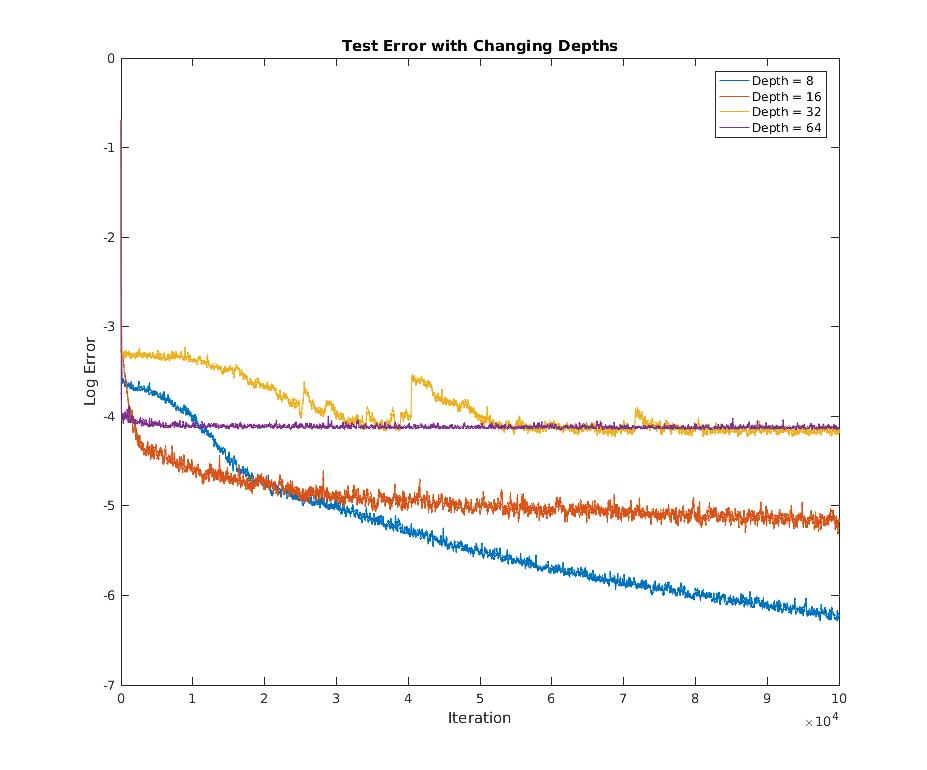
\includegraphics[width = 1.6in]{plotChangeDepth.jpg}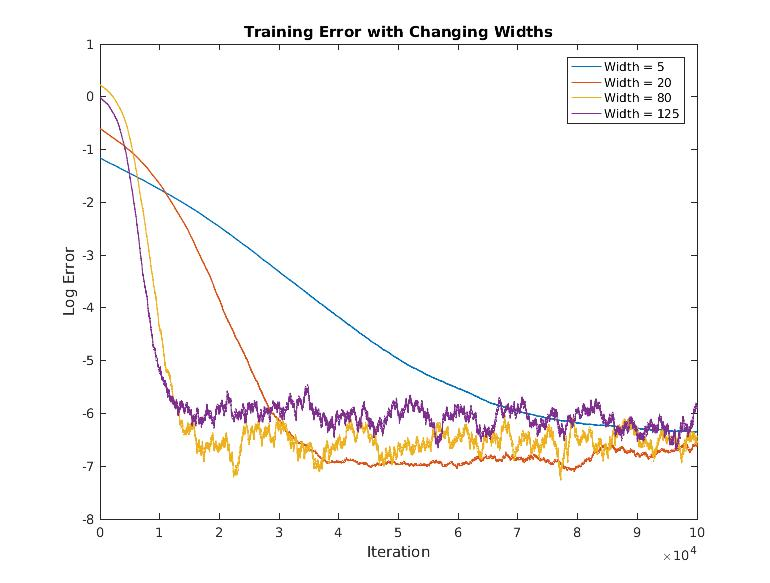
\includegraphics[width = 1.77in]{plotChangeWidth.jpg}
\caption{Left:Test Error of Networks of Varying Depth. Right: Test Error of Networks of Varying Width.}
\end{center}
\vskip -0.1in
\end{figure}
We note that we have been using training error as a measure of success, but it's possible that the true underlying parameters are not learned. If our loss function were strongly convex, small training error would imply a small norm in the parameter space. For the sign activation function, we can show a related result.

\Anote{there is a main theorem in your experimental section. you should move this to one of your section on ``other potentials''.}
\begin{restatable}{theorem}{signUnique}
\label{SignUnique}
Let $\mathcal{M} = S^{d-1}$ and $\sigma$ be the sign activation function and $b_2,...,b_k = 0$. If the loss \eqref{errLoss} at $(\boldsymbol{a,\theta})$ is less than $O(1)$, then there must exist $\theta_i$ such that $w_1^T\theta_i > \Omega(1/\sqrt{k})$.
\end{restatable}




\section{Conclusion}

We studied the problem of learning a function using a neural network of a certain depth and width assuming it can
be represented using such a network.   We show that for networks of depth two with certain simplifying assumptions  the question of whether the gradient descent converges to the desired target function is equivalent to a certain question of convergence in electrodynamics.  Given $n$  fixed protons and $n$ mobile under the influence of the electrical force of attraction from the protons and repulsion from the remaining electrons will all the electrons will be matched up all the protons upto some permutation. Based on this equivalance, we proved the existence of an activation function such that the corresponding gradient descent dynamics result in learning at least one of the hidden nodes in the target network. 


%In this work, we view deep learning of neural networks in the context of electron-proton dynamics and analyzed the convergence of the underlying weight parameters of the neural network using arguments inspired from physics and non-convex optimization. To do so, we first established mathematical relationship between activation functions and their corresponding potentials. Next, we interpreted gradient descent as electrodynamics under a certain potential. Finally, we discovered classes of activation functions that give rise to positive convergence results, some of which relate to very commonplace activations, such as the sign and polynomial. For these classes of depth-2 neural networks, our results imply that they are provably learnable by deep learning. Our experiments seem to imply that higher depth neural networks are not learnable. 

%However, 
We believe that convergence results for depth-2 neural networks can be extended to even more activation functions, such as the sigmoid or the ReLU. Also, we believe these convergence results can be proven with minimal assumptions.


{\small
\bibliography{biblio}
\bibliographystyle{unsrt}}

\newpage
\appendix
% 
\section{Runtime Bounds with Stochastic Gradients}
\Anote{this section should start with a definition, then have a main theorem that provides, as you presage, ``runtime bounds with stochastic gradient''. as it stands, i can't find such a theorem. i see lots of little claims though. please provide a main theorem at the top, and rename everything else to ``lemma''.}

The gradient descent convergence results in the previous sections lay
the foundation for reasoning about the convergence of stochastic
gradient descent (SGD). To derive finite runtime bounds, we need to
address three technical details: 1) realizable potentials are only
approximately strictly subharmonic or $\lambda$-harmonic, 2) the
variance of the stochastic gradient and 3) SGD should escape local
minima in a bounded (hopefully polynomial) number of iterations. The
second and third detail are analyzed with standard techniques in
optimization and statistics: the former requires generalization bounds
for neural networks and the latter requires a lower bound on the
negative curvature, which leads to the follow definition.
%
\begin{definition} 
Let $\Omega \subseteq \R^d$. A point $x^*$ is a
  {\bf $\epsilon$-strict} point of $f : \Omega \to \R$ if f is twice
  differentiable at $x^*$ and
  $\lambda_{min}(\nabla^2f(x^*)) < -\epsilon$
\end{definition}

Note that if a critical point is not a local minimum, then it is
$0$-strict. By reusing techniques in \cite{GeHJY15}, we show that SGD (with noise) can avoid all points that are $\epsilon$-strict in $\poly(1/\epsilon)$ iterations. Intuitively, this means that SGD will converge to points with small gradient and small negative curvature, converging to a point in $\mathcal{M}_\epsilon$, where 
%
\[\mathcal{M}_{L, \epsilon} = \left\{x\in \mathcal{M} \Big| \|\nabla L(x)\|
  \leq \epsilon \text{ and } \lambda_{min}(\nabla^2 L(x)) \geq
  -\epsilon\right\}\]
%
We note that the more straightforward algorithm of computing the negative descent direction of the Hessian is possible. The full description and proof of our SGD algorithm is given in the supplementary material. 

We now discuss convergence results for a almost $\lambda$-harmonic function on $S^{d-1}$ that is constructed in the following theorem. The construction is technical and requires the Hermite polynomial basis in Theorem \ref{thm:rotReal}.
%
\begin{definition}
$\Phi(\theta, w)$ is $m$-almost $\lambda$-harmonic on $S^{d-1}$ if for
all $\theta, w\in S^{d-1}$, $|\Delta_{\theta}\Phi(\theta, w) - \lambda \Phi (\theta,w)| \leq \poly(m)|\theta^Tw|^m$ 
\end{definition}


\begin{restatable}{lemma}{almostHarmonic}\label{AlmostHarmonic}
For any $m$, we can construct a realizable odd $m$-almost 1-harmonic potential, $\Phi_m$, that corresponds to a odd polynomial $\sigma$ of degree $m$. Furthermore, $|\Phi_m(\theta^Tw)|\leq 1$ for all $\theta, w \in S^{d-1}$.
\end{restatable} \Snote{Can you generalize this theorem to $\lambda$-harmonic?}
%
%
\begin{restatable}{lemma}{bounded}
\label{bounded}
  Let $L$ be as in Eq.~\eqref{errLoss} and let $b_1,...,b_k$ be reals
  bounded by $\poly(d)$ and $|\Phi|\leq 1$ on $\mathcal{M}$. Let
  $G = L + \beta\|a\|^2$. Then, if
  $G(\boldsymbol{a,\theta}) \leq G(0,\boldsymbol{\theta})$, then
  $\|a\| \leq \poly(d)/\beta$.
\end{restatable}
%
%
\begin{restatable}{lemma}{eigConv}
\label{eigConv}
Let $\mathcal{M} = S^{d-1}$ and let $b_1,...,b_k$ be reals bounded by
$\poly(d)$. For all $\epsilon \in (0,1),$ we can pick
$m = O(\log(d)\log(1/\delta)/\epsilon)$ such that the following holds:

Let $L$ be as in \eqref{errLoss} with an $m$-almost 1-harmonic
potential $\Phi_m$ and let $G = L + \|a\|^2$.  If
$(\boldsymbol{a,\theta}) \in \mathcal{M}_{G, \delta^2 / (4d)}$ and
$G(\boldsymbol{a,\theta}) \leq G(0,\boldsymbol{\theta})$, then for all
$i$, either there exists $j$ such that
$|w_j^T\theta_i| > 1- k^2\epsilon,$ or $|a_i| < \delta$.
\end{restatable}
%
\begin{proof}
  The proof is similar to Theorem \ref{EigStrict}. Consider all
  $\theta_i$ such that $|a_i| > \delta$ and
  $|w_j^T\theta_i| \leq 1-\epsilon$ for all $j$. WLOG, let these be
  $\theta_1,...,\theta_l$, for some $l \leq k$. Assume for now that
  furthermore, $|\theta_i^T\theta_j| \leq 1-\epsilon$ for
  $i \leq l, j\geq l+1$.  Then, consider a correlated rotation on the
  sphere, which is a correlated translation in spherical
  coordinates. So, consider the loss function 
%
\[ H({\bf a, v}) = G({\bf a,\theta_1+v,...,\theta_l+v},\theta_{l+1},..\theta_k)\]

Let $(\boldsymbol{a,\theta}) \in \mathcal{M}_{G, \delta^2/(4d)}$. Then,
the optimality conditions on ${\bf a}$ are as usual:
%
\begin{align*}
   \abs{\pd{H}{a_i}} & = \lvert 2\sum_{j=1}^k b_j \Phi_m(\theta_i^T w_j) +
    2\sum_{j: j\neq i} a_j \Phi_m(\theta_i^T\theta_j) \\
& \qquad \qquad \qquad + (2\Phi_m(1) +
    2)a_i \rvert \\
& \leq \delta 
\end{align*}
%
Since $\Phi_m$ is $m$-almost 1-harmonic, we get,
%
\begin{align*}
  &  \left| \Delta_{{\bf v}} H -  2\sum_{i=1}^l\sum_{j=1}^k a_i b_j
    \Phi_m(\theta_i^Tw_j) \right. \\
& \qquad \qquad \qquad \left.- 2\sum_{i=1}^l\sum_{j= l+1}^k
  a_ia_j(-\Phi_m(\theta_i^T\theta_j)) \right| \\
  & \leq   2\poly(m)\left(\sum_{i=1}^l\sum_{j=1}^k a_i b_j  |\theta_i^Tw_j|^m+\sum_{i=1}^l\sum_{j= l+1}^k a_ia_j|\theta_i^T\theta_j|^m\right)
\end{align*}
%
Together, we get
%
\begin{align*}
& |\Delta_{{\bf v}}H + \sum_{i=1}^l (2\Phi_m(\theta_i^T\theta_i)+2)a_i^2 + 2\sum_{i \neq j}^l a_ia_j\Phi_m(\theta_i^T\theta_j)| \\
& \leq \sum_{i=1}^l\delta |a_i| +\sum_{i=1}^l 2|a_i|\poly(m)|\sum_{j=1}^k b_j
  (\theta_i^Tw_j)^m +  \sum_{j=l+1}^k  a_j(\theta_i^T\theta_j)^m|
\\
\end{align*}

Again, since these inner products are assumed to be less than
$1-\epsilon$ and and $\|a\| \leq \poly(d)$ by
$G(\boldsymbol{a,\theta}) \leq G(0,\boldsymbol{\theta})$ and Lemma
\ref{bounded}, we can choose
$m = O(\frac{1}{\epsilon}\log(d)\log(1/\delta))$ large enough such
that
%
\begin{align*}
 2\poly(m)\sum_{i=1}^l|\sum_{j=1}^k b_j (\theta_i^Tw_j)^m +
  \sum_{j=l+1}^k  a_j(\theta_i^T\theta_j)^m| \\
 \leq  2\poly(d,k,m)e^{-\epsilon m} \leq \delta/2
\end{align*}

Finally, consider the following expression
%
\begin{align*}
D & = \expt\left[\left( \sum_{i=1}^l a_i \sigma(\theta_i,X)\right)^2\right] \\
%
& =\sum_{i=1}^l a_i^2\Phi_m(\theta_i^T\theta_i) + \sum_{i \neq j}^l
  a_ia_j\Phi_m(\theta_i^T\theta_j)
\end{align*}
%
Since $D \geq 0$ and combined with the fact that $|a_i| > \delta$,
%
\begin{align*}
\Delta_{{\bf v}}H & \leq  \sum_{i=1}^l (-2a_i^2 +\delta |a_i|+(\delta/2)|a_i|) \\
& \leq   \sum_{i=1}^l  |a_i|(-2\delta + 3\delta/2) < -l\delta^2/4
\end{align*}

Since the Laplacian is a sum of $d$ eigenvalues, this implies that we can find $u \in S^{d-1}$ such that $-l\delta^2/(4d) > u^T\nabla^2_v H u$. Finally, notice that if $w = (\underbrace{u,...u}_{l {\textrm{ times}}},0,...,0)$, then $w^T\nabla^2_{\boldsymbol{\theta}} G w = u^T\nabla^2_v H u < -l\delta^2/4d$. Since $w$ has $\|w\|^2 = l$, we conclude that $(\boldsymbol{a,\theta})$ is $\delta^2/(4d)$-strict, contradicting that it is in $\mathcal{M}_{G, \delta^2/(4d)}$. 

Finally, it must be the case that there exists $\theta_{j_1},...\theta_{j_l}$ such that
$|\theta_i^T\theta_{j_1}| > 1-\epsilon$ and
$|\theta_{j_{i}}^T\theta_{j_{i+1}}| > 1-\epsilon$, and
$|\theta_{j_l}^Tw_j| > 1-\epsilon$ for some $w_j$. Therefore,
$|\theta_i^Tw_j| > 1- k^2\epsilon$. 
\end{proof}

\begin{theorem}\label{eigRes}
  Assume the conditions of Theorem~\ref{eigConv}. If
$G({\bf a, \boldsymbol{\theta}}) \leq G(0,\boldsymbol{\theta}) - 2\delta\sqrt{G(0,\boldsymbol{\theta})}$
  and $(\boldsymbol{a,\theta}) \in \mathcal{M}_{G,\delta^2/(4\poly(d))}$,
  then there exists some $i, j$ such that $\theta_i$ is in an
  $\epsilon$-neighborhood of $w_j$.
\end{theorem}
 
 \begin{proof}
   By Lemma \ref{eigConv}, if there does not exists $i, j$ such that
   $|w_j^T\theta_i| > 1-k^2\epsilon$ is if for all $\theta_i$, then
   $|a_i| < \delta/\poly(d)$ for all $i$. Now, for a integrable
   function $f(x)$, $\| f\|_X = \sqrt{\expt_X[f(X)^2]}$ is a
   norm. Therefore, if $f(x) = \sum_i b_i \sigma(w_i,x)$ be our true
   target function, we conclude that by triangle inequality
\begin{align*}
\sqrt{G(\boldsymbol{a,\theta})}  & \geq \norm{\sum_{i=1}^k a_i \sigma(\theta_i,x) - f(x)}_X \\
&\geq \|f(x)\|_X\ - \sum_{i=1}^k \|a_i\sigma(\theta_i,x) \|_X \\
& \geq
  \sqrt{G(0,\boldsymbol{\theta})} - \delta
\end{align*}
Squaring gives a contradiction, so we conclude that there must exist $i, j$ such that $\theta_i$ is in a $k^2\epsilon$ neighborhood of $w_j$.
 \end{proof}
 
 \begin{observation}\label{initialize}
Let $\theta_1$ be chosen uniformly from $\mathcal{M}$ and assume
\[ \expt\left[\left(  \sum_{j=1}^k b_j \Phi(\theta_1,w_j)\right)^2\right] > 5\delta\sqrt{L(0,0)}\] 

Then, we can initialize $\boldsymbol{a,\theta}$ such that $G({\bf a, \boldsymbol{\theta}}) \leq G(0,\boldsymbol{\theta}) - 2\delta\sqrt{G(0,\boldsymbol{\theta})}$ with high probability.
 \end{observation}
 
 \begin{proof}
   Consider choosing $\theta_1$ uniformly from $\mathcal{M}$ and then
   optimizing $a_1$. Notice that the expected loss decrease is:
%
\begin{align*}
  \expt[ G(a_1,\theta_1)] - G(0,0) & = \expt\left [\min_{a_1} 2a_1^2 +
  2\sum_{j=1}^k a_1 b_j\Phi(\theta_1,w_j)\right] \\
 %
 & = -\frac{1}{2}\expt\left[\left(  \sum_{j=1}^k b_j
   \Phi(\theta,w_j)\right)^2\right] 
\end{align*}
Let
$h(\theta) = \sum_i b_i \Phi(\theta, w_i)$. Since $a_i,b_i, \Phi$ are
$\poly(d)$-bounded, our random variable $h(\theta)$ is
$\poly(d)$-bounded. From Hoeffding bounds, we see that after
$\poly(d,1/\delta)$ samples, we know that
$\hat{\expt}h(\theta)^2 \geq 2\delta\sqrt{G(0,0)}$, where
$\hat{\expt}$ denotes the empirical average over $\theta$. Therefore,
we must have found some $\theta$ such that
$h(\theta)^2 \geq 2\delta \sqrt{G(0,0)}$. Therefore,
$G(\boldsymbol{a,\theta}) - G(0,0) \leq 2\delta \sqrt{G(0,0)}$.
\end{proof}
 
\begin{lemma}\label{largeVariance}
  Let $\Phi_m$ be as in \ref{AlmostHarmonic} \Snote{Always say
    Lemma/Theorem when referring to one. So this should be
    Lemma~\ref{AlmostHarmonic}} and let $\theta, w_1,...,w_k$ be
  independent and uniformly randomly chosen on $S^{d-1}$. Then, over
  $\theta, w_1,...,w_k$,
 
 $\expt\left[\left(  \sum_{j=1}^k b_j \Phi(\theta,w_j)\right)^2\right]
 \geq \norm{b}_2^2 \cdot \Omega(1/m).$
\end{lemma}
%
\begin{proof}
Note that $\Phi_m$ is a degree $m$ polynomial with non-negative coefficients and it only has odd-degree terms. Since it is odd, $E[\Phi_m(\theta^Tw_i)] = 0$ and the cross terms in the expansion of the square vanish:
%
\[ \expt\left[\left(  \sum_{j=1}^k b_j
     \Phi_m(\theta^Tw_j)\right)^2\right] = \sum_{j=1}^k b_j^2 \expt[\Phi_m(\theta^Tw_j)^2]\]

So, it suffices to show $\expt[\Phi_m(\theta,w_j)^2] \geq 1/m$.  Now, since $\Phi_m$ has non-negative coefficients,
\begin{align*}
& \expt[\Phi_m(\theta^Tw_j)^2] = \expt\left[\left(\sum_{i=1, i \,
                               odd}^m c_i
                               (\theta^Tw_j)^i\right)^2\right] \\
& \qquad = \sum_{i,j \,odd} c_ic_j E[(\theta^Tw_j)^{i+j}] \geq \sum_{i,j
  \,odd}c_i c_j \Omega(1/(i+j))  \\
& \qquad =\Omega(1/m) 
\end{align*}

Where we used the fact that
$\sum_{i,j} c_ic_j = (\sum_i c_i)^2 = \Phi_m(1)^2 = 1$ and
$E[(\theta^Tw_j)^{n}] \geq \Omega(1/n)$, which holds by integration by
parts. \Snote{The last claim is not correct. $(\theta^Tw_j)^n$ is
  $O(1/\sqrt{n})^n$ with high probability.}
\end{proof}

\begin{theorem}
  Let $\mathcal{M} = S^{d-1}$ and let $b_1,...,b_k$ be such that
  $||b||_2$ is $\Omega(1)$ and $O(poly(d))$, and $w_1,..,w_k$ are
  randomly chosen from $\mathcal{M}$. 
  
  With high probability, for all $\epsilon \in (0,1),$ there exists $m, \delta$ (that depends on $d$) such that for the $m$-almost $1$-harmonic potential $\Phi_m$ the
  following holds: we can chose an initial point $(\boldsymbol{a^{(0)}, \theta^{(0)}})$ so that if after running SGD (Algorithm \ref{SGD}) on the regularized objective
  $G(\boldsymbol{a,\theta})$, there exists an $i, j$ such that $|w_j^T\theta_i| > 1- k^2\epsilon$ in $O(poly(d,1/\epsilon))$ iteration complexity and $O(poly(d^{log(d)},1/\epsilon))$ sample complexity.
\end{theorem}

\begin{proof}
We choose $m = O(\log d \log (1/\delta)/\epsilon)$. Combining Observation \ref{initialize} and Lemma \ref{largeVariance}, we can initialize $\boldsymbol{a,\theta}$ such that $G(\boldsymbol{a,\theta}) - G(0,0) \leq 2\delta \sqrt{G(0,0)}$ for $\delta = O(1/m) = \poly(d,1/\epsilon)$ \Rnote{This is not exactly true but correct in expectation..to apply concentration, we need to sample $w_i$ multiple times}.

Next, to use Theorem \ref{strongConverge}, we check the regularity conditions. By assumption, we can choose $B, L, \rho$ to be $\poly(d,1/\epsilon)$ since $\Phi$ and the second and third partials of $\Phi$ are all bounded by $\poly(d,1/\epsilon)$ in $\mathcal{M}$. Furthermore, our activation function $\sigma$ and its derivatives are bounded in magnitude by $c|x|^{m}$, where $m = O(\log d \log (1/\delta)/\epsilon)$ and by \cite{Hermite}, we can let $c = O(m^m)$. By Theorem \ref{genErrBound}, with high probability, we can construct a stochastic oracle up to $\epsilon$ error with sample complexity $\poly(d^{\log(d)},1/\epsilon)$. Therefore, we conclude by Theorem \ref{strongConverge} that we are in $\mathcal{M}_{G,\delta^2/(4\poly(d))}$ in $\poly(d,1/\epsilon)$ iterations. Finally, we conclude by Theorem \ref{eigRes}.
\end{proof}











 \if{1}
 In the end, we can combine Theorem \ref{eigRes} with Algorithm \ref{GDReset} to derive a convergence result.
 
 \begin{algorithm}[tb]
 \caption{SGD Algorithm with Resets}
   \label{GDReset}
\begin{algorithmic}
  \STATE {\bfseries Input:}
  $(\boldsymbol{a,\theta}) = (a_1,...,a_k,\theta_1,...,\theta_k), a_i
  \in\R, \theta_i\in\mathcal{M}$;
  $T\in \N$; $\widehat{L}$; $\alpha\in \R$; $\delta \in \R$;
  $\gamma \in R$; $S \in \R$ \vspace{0.1in} 
  \FOR{$i=1$ {\bfseries to} $S$} 
  \STATE $(\boldsymbol{a},\boldsymbol{\theta}) = SGD \left(\widehat{L}, (\boldsymbol{a},\boldsymbol{\theta}),T, \alpha,\delta \right)$
  \IF{(ii) or (iii)}
    \STATE remove clump
    \REPEAT \STATE Sample $\theta_i$
  uniformly from $\mathcal{M}$
  \UNTIL{$\left (\frac{\partial
        \widehat{L}(\boldsymbol{a,\theta})}{\partial a_i} \right)^2
    \geq \gamma$}
    \ELSE \STATE  {\bf return} $(\boldsymbol{a}, \boldsymbol{\theta}) $
      \ENDIF
    \ENDFOR
   \STATE {\bf return} $(\boldsymbol{a}, \boldsymbol{\theta}) $
   \end{algorithmic}
\end{algorithm}

\begin{theorem}
For any $0 < \epsilon < 1$, we can construct a realizable potential $\Phi$ such that with high probability, running Algorithm \ref{GDReset} on \eqref{errLoss} with error $\delta = \poly(\epsilon,1/d)$, $\gamma = \epsilon$ and stepsize $\alpha = 1/\poly(d,1/\epsilon)$ converges in $T = \poly(d, 1/\epsilon)$ iterations to $(\boldsymbol{a,\theta})$ such that each $\theta_i$ is within $\epsilon$-neighborhood of some $w_j$ or there exists $i$ such that if $\theta_i$ is picked uniformly in $\mathcal{M}$
%
\[ \expt\left[\left( \sum_{j < i} a_j \Phi(\theta_i,\theta_j) + \sum_{j=1}^k b_j \Phi(\theta_i,w_j)\right)^2\right] < \epsilon\]
\end{theorem}

\begin{proof}


\end{proof}
\fi


%%% Local Variables:
%%% mode: latex
%%% TeX-master: "icmlpaper2017.tex"
%%% End:
\section{Electron-Proton Dynamics}

\epdyn*

\begin{proof}
The initial values are the same. Notice that continuous gradient descent on $L(\boldsymbol{a,\theta})$ with respect to $\theta$ produces dynamics given by $\frac{d\theta_i(t)}{dt} = -\nabla_{\theta_i}L(\boldsymbol{a,\theta})$. Therefore,
\[\frac{d\theta_i(t)}{dt} = -2\sum_{j \neq i} a_i a_j
\nabla_{\theta_i}\Phi(\theta_i,\theta_j) - 2\sum_{j=1}^k
a_ib_j\nabla_{\theta_i} \Phi(\theta_i,w_j)\] 
And gradient descent does not move $w_i$. By definition, the dynamics corresponds to Electron-Proton Dynamics as claimed.
\end{proof}

\section{Realizable Potentials}
\label{realizable}

\subsection{Activation-Potential Calculations}
First define the {\it dual} of a function $f: \R \to \R$ is defined to be 
%
\[ \widehat{f}(\rho) = \expt_{X,Y \sim N(\rho)}[f(X)f(Y)],\]
%
where $N(\rho)$ is the bivariate normal distribution with $X, Y$ unit variance and $\rho$ covariance. This is as in \cite{DanielyFS16}.
%
\begin{lemma}\label{rotLem}
Let $\mathcal{M} = S^{d-1}$ and $\sigma$ be our activation function, then $\widehat{\sigma}$ is the corresponding potential function.
\end{lemma}

\begin{proof}
If $u, v$ have norm 1 and if $X$ is a standard Gaussian in $\R^d$, then note that $X_1 = u^TX$ and $X_2 = v^TX$ are both standard Gaussian variables in $\R^1$ and the covariance is $E[X_1X_2] = u^Tv$. 

Therefore, the dual function of the activation gives us the potential function.
\begin{align*}
\expt_{X}[\sigma(u^TX)\sigma(v^TX)] & =
\expt_{X,Y \sim N(u^Tv)}[\sigma(X)\sigma(Y)] \\
& = \widehat{\sigma}(u^Tv).
\end{align*}
\end{proof}

By Lemma \ref{rotLem}, the calculations of the activation-potential
for the sign, ReLU, Hermite, exponential functions are given in
\cite{DanielyFS16}. For the Gaussian and Bessel activation functions,
we can calculate directly. In both case, we notice that we may write
the integral as a product of integrals in each dimension. Therefore,
it suffices to check the following 1-dimensional identities.
\begin{align*}
  & \int_{-\infty}^\infty
    \sqrt{2}e^{x^2/4}e^{-(x-\theta)^2}\sqrt{2}e^{x^2/4}e^{-(x-w)^2} \frac{1}{\sqrt{2\pi}} e^{-x^2/2}\, dx \\
  & \qquad = \sqrt{\frac{2}{\pi}}\int_{-\infty}^\infty
    e^{-(x-\theta)^2}e^{-(x-w)^2} \, dx = e^{-(\theta -w)^2/2}
\end{align*}
\begin{align*}
& \int_{-\infty}^\infty (\frac{2}{\pi})^{3/2}e^{x^2/2}K_0(|x-\theta|)K_0(|x-w|)  \frac{1}{\sqrt{2\pi}} e^{-x^2/2}\, dx \\
& \qquad 
= \int_{-\infty}^\infty \frac{2}{\pi^2}K_0(|x-\theta|)K_0(|x-w|) \, dx
  = e^{-|\theta -w|}
\end{align*}


The last equality follows by Fourier uniqueness and taking the Fourier transform of both sides, which are both equality $\sqrt{2/\pi}(\omega^2+1)^{-1}$. 


\subsection{Characterization Theorems}

\begin{definition}
A potential $\Phi$ is $\FT$-integrable if it is square-integrable and $\FT({\Phi}(\omega))$ is integrable, where $\FT$ is the standard Fourier transform.
\end{definition}

\tranReal*

\begin{proof}
Since $\Phi$ is square-integrable, its Fourier transform exists. Let $h(x) = \FT^{-1}(\sqrt{\FT(\Phi)})(x)$ and this is well-defined since the Fourier transform was non-negative everywhere and the Fourier inverse exists since $\sqrt{\FT(\Phi)}(x)$ is square-integrable. Now, let $\sigma(x,w) = (2\pi)^{1/4}e^{x^2/4}h(x-w)$. Realizability follows by the Fourier inversion theorem:
%
\begin{align*}
    \expt_{X \sim N}[\sigma(X,w)\sigma(X,\theta)]  &= \int_{\R^n} h(x-w)h(x-\theta) \, dx \\
    &= \int_{\R^n} h(x)h(x-(\theta-w)) \, dx \\
    &= \FT^{-1}(\FT(h\ast h)(\theta -w)) \\
    &= \FT^{-1}(\FT(h)^2(\theta - w)) \\
    &= \FT^{-1}(\FT(\Phi)(\theta - w)) \\
    &= \Phi(\theta - w) 
\end{align*}
 
Note that $\ast$ denotes function convolution.
\end{proof}




\rotReal*

\begin{proof}
By \ref{rotLem} and due to the orthogonality of hermite polynomials, if $f = \sum_i a_i h_i$, where $h_i(x)$ is the i-th Hermite polynomial, then
%
\[\widehat{f}(\rho) = \sum_{i} a_i^2 \rho^i\]

Therefore, any function with non-negative taylor coefficients is a valid potential function, with the corresponding activation function determined by the sum of hermite polynomials, and the sum is bounded almost everywhere by assumption.
\end{proof}

\subsection{Further Characterizations}

To apply Theorem~\ref{thm:tranReal}, we need to check that the Fourier transform of our function is non-negative. Not only is this is not straightforward to check, many of our desired potentials do not satisfy this criterion. In this section, we would like to have a stronger characterization of realizable potentials, allowing us to construct realizable potentials that approximates our desired potential.
 
\begin{definition}
Let $\Phi$ be a positive semidefinite function if for all $x_1,...,x_n$, the matrix $A_{ij} = \Phi(x_i - x_j)$ is positive semidefinite. 
\end{definition}

\begin{lemma}\label{lem:psd}
Let $\mathcal{M} = \R^d$ and $\Phi(\theta, w) = f(\theta-w)$ is is realizable, then it is positive semidefinite.
\end{lemma}

\begin{proof}
If $\Phi$ is realizable, then there exists $\sigma$ such that  $\Phi(\theta, w) =  \expt_{X \sim N}[\sigma(X, w)\sigma(X, \theta)]$. For $x_1,...,x_n$, we note that the quadratic form:
\begin{align*}
\sum_{i,j} \Phi(x_i,x_j) v_i v_j 
& = \sum_{i,j} \expt_{X \sim N}[\sigma(X, x_i)\sigma(X, x_j)] v_i v_j 
 = \expt_{X \sim N}\left[\left(\sum_{i}v_i \sigma(X , x_i) \right)^2\right] \geq 0
\end{align*}

Since $\Phi$ is translationally symmetric, we conclude that $\Phi$ is positive semidefinite.
\end{proof}

\begin{lemma}\label{intReal}
Let $w(x) \geq 0$ be a positive weighting function such that $\int_a^b w(x) \, dx$ is bounded. If $\Phi_x$ is a parametrized family of $\FT$-integrable realizable potentials, then, $\int_a^b w(x) \Phi_x$ is $\FT$-integrable realizable.
\end{lemma}

\begin{proof}
Let $\Phi = \int_a^b w(x) \Phi_x$. From linearity of the Fourier transform and $\int_a^b w(x)\, dx$ is bounded, we know that $\Phi$ is $\FT$-integrable. Since $\Phi_x$ are realizable, they are positive definite by Lemma~\ref{lem:psd} and by Bochner's theorem, their Fourier transforms are non-negative. And since $w(x) \geq 0$, we conclude by linearity and continuity of the Fourier transform that $\FT(\Phi) \geq 0$. By Theorem \ref{thm:tranReal}, we conclude that $\Phi$ is realizable.
\end{proof}



\begin{lemma}\label{baseConstruct}
Let $\mathcal{M} = \R^d$ for $d \equiv 3 \mod 4$. Then, for any $\epsilon, t > 0$, there exists a $\FT$-integrable realizable $\Phi$ such that for $t \geq r > \epsilon$, $\Phi^{(d-1)}(r) = t -r$ and for $ r \leq \epsilon$, $\Phi^{(d-1)}(r) = \frac{t-\epsilon}{\epsilon}r$. Furthermore, $\Phi^{(k)}(r) = 0$ for $r > t$ for all $0 \leq k \leq d$.
\end{lemma}

\begin{proof}
Our construction is based on the radial activation function $h_t(x, \theta) = \bf{1}_{\|\theta - x\| \leq t/2}$, which is the indicator in the disk of radius $t/2$. This function, when re-weighted correctly as $\sigma_t(x,\theta) =  (2\pi)^{1/4} e^{x^2/4}h_t(x,\theta)$ gives rise to a radial potential function that is simply the convolution of $h_t$ with itself, measuring the volume of the intersection of two spheres of radius $t$ centered at $\theta$ and $w$.
%
\begin{align*}
\Phi_t(\theta, w) & = \expt_X[\sigma_t(X,\theta)\sigma_t(X,w)]
= \begin{cases}
C\int_{\|\theta - w\|/2}^{t/2} ((t/2)^2 - x^2)^{(d-1)/2} \, dx & \|\theta - w\| \leq t\\
0 & \textrm{ otherwise.}
\end{cases}
\end{align*}
%
Therefore, as a function of $r=\|\theta - w \|$, we see that when $r \leq t$, $\Phi_t(r) = C\int_{r/2}^{t/2} ((t/2)^2-x^2)^{(d-1)/2} \, dx$ and $\Phi_t'(r) = -C'((t/2)^2-(r/2)^2)^{(d-1)/2}$. Since $d \equiv 3 \mod 4$, we notice that $\Phi_t'$ has a positive coefficient in the leading $r^{d-1}$ term and since it is a function of $r^2$, it has a zero $r^{d-2}$ term. Therefore, we can scale $\Phi_t$ such that 
\begin{align*}
\Phi_t^{(d-1)}(r) = \begin{cases}
r & r \leq t\\
0 & \textrm{ otherwise.}
\end{cases} 
\end{align*}

$\Phi_t$ is clearly realizable and now we claim that it is $\FT$-integrable. First, $\Phi_t$ is bounded on a compact set so it is square-integrable. Now, since $\Phi_t = h_t \ast h_t$ can be written as a convolution, $\FT(\Phi_t) = \FT(h_t)^2$. Since $h_t$ is square integrable, then by Parseval's, $\FT(h_t)$ is square integrable, allowing us to conclude that $\Phi_t$ is $\FT$-integrable.

Now, for any $\epsilon > 0$, let us construct our desired $\Phi$ by taking a positive sum of $\Phi_t$ and then appealing to Lemma \ref{intReal}. Consider
%
\[\Phi(r) = \int_{\epsilon}^{t} \frac{1}{x^2}\Phi_x(r) \, dx\]

First, note that the total weight $\int_\epsilon^t \frac{1}{x^2}$ is bounded. Then, when $r \geq t$, since $\Phi_x(r) = 0$ for $x \leq t$, we conclude that $\Phi^{(k)}(r) = 0$ for any $k$. Otherwise, for $\epsilon < r < t$, we can apply dominated convergence theorem to get
\begin{align*}
\Phi^{(d-1)}(r) = \int_{\epsilon}^r \frac{1}{x^2}\Phi_x^{(d-1)}(r) \, dx + \int_{r}^t \frac{1}{x^2} \Phi_x^{(d-1)}(r) \, dx
 = 0 + \int_r^t \frac{r}{x^2} \, dx = 1 -r/t 
\end{align*}

Scaling by $t$ gives our desired claim. For $r\leq \epsilon$, we integrate similarly and scale by $t$ to conclude.
\end{proof}

\begin{lemma}\label{transConstruct}
Let $\mathcal{M} = \R^d$ for $d \equiv 3 \mod 4$ and let $\Phi(r)$ be a radial potential. Also, $\Phi^{(k)}(r) \geq 0$ and $\Phi^{(k+1)}(r)\leq 0$ for all $r > 0$ and $k \geq 0 $ even, and $\lim_{r \to \infty} \Phi^{(k)}(r) = 0$ for all $0 \leq k \leq d$. 

Then, for any $\epsilon > 0$, there exists a $\FT$-integrable realizable potential $\overline{\Phi}$  such that $\overline{\Phi}^{(k)}(r) = \Phi^{(k)}(r)$ for all $0 \leq k \leq d-1$ and $r \geq \epsilon$. Furthermore, we have $\overline{\Phi}^{(d-1)}(r) \geq 0$ for all $r  > 0$ and $\overline{\Phi}^{(k)}(r) \geq 0$ and $\overline{\Phi}^{(k+1)}(r)\leq 0$ for all $r > 0$ and $d - 3 \geq k \geq 0 $ even.

Lastly, for $r < \epsilon$ and $0 \leq k \leq d-1$, $|\overline{\Phi}^{(d-1-k)}(r)| \leq |\Phi^{(d-1-k)}(\epsilon)| + \sum_{j=1}^k \frac{(\epsilon - r)^{k-j+1}}{(k-j+1)!} |\Phi^{(d-j)}(\epsilon)|$
\end{lemma}

\begin{proof}
By Lemma \ref{baseConstruct}, we can find $\Phi_t$ such that
\begin{align*}
\Phi_t^{(d-1)} = \begin{cases}
\frac{t-\epsilon}{\epsilon } r & 0 \leq r \leq \epsilon \\
t - r & \epsilon < r \leq t \\
0 & r > t
\end{cases}
\end{align*}

Furthermore, $\Phi_t^{(k)}(r) = 0$ for $r > t$ for all $0 \leq k \leq d$.
Therefore, we consider 
%
\[\overline{\Phi}(r) = \int_{\epsilon}^\infty \Phi^{(d+1)}(x) \Phi_x(r) \, dx\] 

Note that this is a positive sum with $\int_{\epsilon}^\infty \Phi^{(d+1)}(x) \, dx = -\Phi^{(d)}(\epsilon) < \infty$. By the non-negativity of our summands, we can apply dominated convergence theorem and Fubini's theorem to get
\begin{align*}
\overline{\Phi}^{(d-1)}(r) & = \int_{\epsilon}^\infty  \Phi^{(d+1)}(x) (\Phi_x^{(d-1)}(r)) \, dx \\
& = \int_{r}^\infty  \Phi^{(d+1)}(x) (\Phi_x^{(d-1)}(r)) \, dx \\
& = \int_r^\infty \Phi^{(d+1)}(x) \int_r^x 1 \, dy \,dx  \\
& = \int_r^\infty \int_y^\infty \Phi^{(d+1)}(x) \, dx \, dy = \int_r^\infty  -\Phi^{(d)}(y) \, dy \\
& = \Phi^{(d-1)}(r)
\end{align*}

Now, since $\overline{\Phi}^{(d-1)}(r) = \Phi^{(d-1)}(r)$ for $r\geq \epsilon$ and $\lim_{r\to\infty} \overline{\Phi}^{(k)}(r) = \lim_{r\to\infty} {\Phi}^{(k)}(r) = 0$ for $0 \leq k \leq d-1$, repeated integration gives us our claim. 

Finally, for the second claim, notice that for $r \leq \epsilon$, we get
\begin{align*}
\overline{\Phi}^{(d-1)}(r) = \int_{\epsilon}^\infty  \Phi^{(d+1)}(x) (\Phi_x^{(d-1)}(r)) \, dx
=  r \int_\epsilon^\infty \Phi^{(d+1)}(x) \frac{x - \epsilon}{\epsilon} \, dx = Cr  
\end{align*}

Note that our constant $C \geq 0$ since the summands are non-negative. Therefore, we conclude that $\overline{\Phi}^{(d-1)}(r) \geq 0$ for all $r > 0$. Repeated integration and noting that $\lim_{r\to\infty} \overline{\Phi}^{(k)}(r) = 0$ for $0 \leq k \leq d-1$ gives us our claim.

Lastly, we prove the last claim of the theorem with induction on $k$. This holds trivially for $k = 0$ since $\overline{\Phi}^{(d-1)}(r) \leq \overline{\Phi}^{(d-1)}(\epsilon) = \Phi^{(d-1)}(\epsilon)$ for $r \leq \epsilon$. Then, assume we have the inequality for $k < d-1$. By integration, we have
\begin{align*}
|\overline{\Phi}^{(d-k-2)}(r)| & \leq |\overline{\Phi}^{(d-k-2)}(\epsilon)| + \int_r^\epsilon |\overline{\Phi}^{(d-1 -k)}(y)| \, dy \\
& \leq |\overline{\Phi}^{(d-k-2)}(\epsilon)| + \int_r^\epsilon |\overline{\Phi}^{(d-1 -k)}(\epsilon)| \, dy \\
& + \int_r^\epsilon \sum_{j=1}^k \frac{(\epsilon -y)^{k-j+1}}{(k-j+1)!}|\Phi^{(d-j)}(\epsilon)| \, dy \\
& \leq  |\overline{\Phi}^{(d-k-2)}(\epsilon)| + \sum_{j=1}^{k+1}  \frac{(\epsilon -y)^{k-j+2}}{(k-j+2)!}|\Phi^{(d-j)}(\epsilon)|
\end{align*}

Therefore, we conclude with induction.
\end{proof}

\AlmostHarmReal*

\begin{proof}
Consider a potential of the form $\Phi(r) = p(r)e^{-\sqrt{\lambda}r}/r^{d-2}$. We claim that there exists a polynomial $p$ of degree $k = (d-3)/2$ with non-negative coefficients and $p(0) = 1$ such that $\Phi$ is $\lambda$-harmonic. Furthermore, we will also show along the way that $p(r) \leq (1+\sqrt{\lambda}r)^d$.

When $d = 3$, it is easy to check that $\Phi(r) = e^{(-\sqrt{\lambda})r}/r$ is our desired potential. Otherwise, by our formula for the radial Laplacian in $d$ dimensions, we want to solve the following differential equation:

\[\Delta \Phi =  \frac{1}{r^{d-1}} \frac{\partial}{\partial r} (r^{d-1} \frac{\partial \Phi}{\partial r}) =\lambda \Phi\]

Solving this gives us the following second-order differential equation on $p$

\[rp'' - (d-3+2\sqrt{\lambda}r)p' +\sqrt{\lambda} (d-3)p = 0\]

Let us write $p(r) = \sum_{i=0}^k a_i r^i$. Then, substituting into our differential equation gives us the following equations by setting each coefficient of $r^i$ to zero:

$r^i$:  $a_{i+1}(i+1)(i - (d-3)) = a_i \sqrt{\lambda} (2i-(d-3))$

$r^k:$ $(-2k +d-3)a_k = 0$

The last equation explains why we chose $k = (d-3)/2$, so that it is automatically zero. Thus, setting $a_0 = 1$ and running the recurrence gives us our desired polynomial. Note that the recurrence is valid and produces positive coefficients since $i < k  = (d-3)/2$. Our claim follows and $\Phi$ is $\lambda$-harmonic. And furthermore, notice that $a_{i+1} \leq \sqrt{\lambda} a_i \leq (\sqrt{\lambda})^{i+1}$. Therefore, $p(r) \leq (1+r\sqrt{\lambda})^d$. 

Lastly, we assert that $\Phi^{(j)}(r)$ is non-negative for $j$ even and non-positive for $j$ odd. To prove our assertion, we note that it suffices to show that if $\Phi$ is of the form $\Phi(r) = p(r) e^{-\sqrt{\lambda}r}/r^{l}$ for some $p$ of degree $k < l$ and $p$ has non-negative coefficients, then $\Phi'(r) = - q(r) e^{-\sqrt{\lambda}r}/r^{l+1}$ for some $q$ of degree $k+1$ with non-negative coefficients. 

Differentiating $\Phi$ gives:
%
\[\Phi' = \frac{e^{-r}}{r^{l+1}} (rp'(r) - (l + \sqrt{\lambda} r)p(r))\]

It is clear that if $p$ has degree $k$, then $q(r) = (l+\sqrt{\lambda} r)p(r) - rp'(r)$ has degree $k+1$, so it suffices to show that it has non-negative coefficients. Let $p_0,..., p_k$ be the non-negative coefficients of $p$. Then, by our formula, we see that 

$q_0 = l p_0$

$q_i = lp_i - ip_i + \sqrt{\lambda}p_{i-1} = (l-i)p_i + \sqrt{\lambda}p_{i-1}$ 

$q_{k+1} = \sqrt{\lambda} p_k$

Since $i \leq k < l$, we conclude that $q$ has non-negative coefficients. Finally, our assertion follows with induction since $\Phi^{(0)}(r)$ is non-negative and has our desired form with $k = (d-3)/2 < d-2$. By Lemma \ref{transConstruct}, our primary theorem follows, we can construct a realizable radial potential $\Phi_\epsilon(r)$ that is $\lambda$-harmonic when $r \geq \epsilon$ and has alternating-signed derivatives.

Lastly, we prove the following preliminary bound on $\Phi_\epsilon^{(k)}(r)$ when $k \leq d$: $|\Phi_\epsilon^{(k)}(r)| \leq 3(2d + \epsilon \sqrt{\lambda})^{2d}\epsilon^{-2d}  $ for all $0 \leq k \leq d-1$. First, notice that by the results of Lemma~\ref{transConstruct}, $\Phi_\epsilon^{(k)}(r)$ is monotone and $\lim_{r\to\infty}\Phi_\epsilon^{(k)}(r) = 0$. So, it follows that we just have to bound $|\Phi_{\epsilon}^{(k)}(0)|$. From our construction, $\Phi_{\epsilon}^{(k)}(\epsilon) = p_k(\epsilon)e^{-\sqrt{\lambda}\epsilon}\epsilon^{2-d-k}$, for some polynomial $p_k$. Furthermore, from our construction, we have the recurrence $p_{k}(\epsilon) = (d-2+k + \sqrt{\lambda}\epsilon)p_{k-1}(\epsilon) - \epsilon p_{k-1}'(\epsilon)$. Therefore, we conclude that for $k \leq d$, $p_k(\epsilon) \leq (2d + \sqrt{\lambda} \epsilon)^kp_0(\epsilon) \leq  (2d + \sqrt{\lambda} \epsilon)^k(1+\sqrt{\lambda}\epsilon)^d \leq (2d + \sqrt{\lambda}\epsilon)^{2d}$. 

Therefore, we can bound
 $|\Phi_\epsilon^{(k)}(\epsilon)| \leq (2d + \sqrt{\lambda}\epsilon)^{2d}\epsilon^{-2d}$. Finally, by Lemma~\ref{transConstruct}, 
\begin{align*}
|\Phi_{\epsilon}^{(d-1-k)}(0)| 
& \leq |\Phi_{\epsilon}^{(d-1-k)}(\epsilon)| + \sum_{j=1}^k \frac{(\epsilon )^{k-j+1}}{(k-j+1)!} |\Phi^{(d-j)}(\epsilon)| \\
& \leq (2d + \sqrt{\lambda}\epsilon)^{2d}\epsilon^{-2d} (1 + \sum_{j=1}^k \frac{\epsilon^{k-j+1}}{(k-j+1)!}) \\
& \leq (2d + \sqrt{\lambda}\epsilon)^{2d}\epsilon^{-2d} e^{\epsilon} \leq 3(2d + \sqrt{\lambda}\epsilon)^{2d}\epsilon^{-2d} 
\end{align*}

And for $r \geq \epsilon$, we see that $|\Phi_\epsilon(r)| = |\Phi(r)| \leq |p(r)|\frac{e^{-\sqrt{\lambda}r}}{r^{d-2}} = (1+r\sqrt{\lambda})^de^{-\sqrt{\lambda}r}r^{2-d}$. And $|\Phi_\epsilon'(r)| = |\Phi'(r)| \leq |p_1(r)| \frac{e^{-\sqrt{\lambda} r}}{r^{d-1}} \leq (d+\sqrt{\lambda}r)(1+ r\sqrt{\lambda})^de^{-\sqrt{\lambda} r} r^{1-d}$.


Finally, we consider the normalized potential: $\widetilde{\Phi}_\epsilon = {\Phi}_\epsilon/{\Phi}_\epsilon(0)$. Note that since ${\Phi}_\epsilon$ is monotonically decreasing, we can lower bound ${\Phi}_\epsilon(0) \geq {\Phi}_\epsilon(\epsilon) \geq e^{-\sqrt{\lambda}}$. Therefore, we can derive the following upper bounds: $|\widetilde{\Phi}_\epsilon^{(k)}(r)| \leq 3(2d + \sqrt{\lambda})^{2d} \epsilon^{-2d}e^{\sqrt{\lambda}}$ and for $r \geq \epsilon$, $|\widetilde{\Phi}_\epsilon(r)| \leq (1+r\sqrt{\lambda})^de^{\sqrt{\lambda}(1-r)}r^{2-d}$ and its derivative is bounded by $|\widetilde{\Phi}_\epsilon'(r)| \leq (d+\sqrt{\lambda}r)(1+ r\sqrt{\lambda})^de^{\sqrt{\lambda}(1- r)} r^{1-d}$.


And lastly, we derive some lower bounds on $\widetilde{\Phi}_\epsilon$ and the first derivative when $r \geq \epsilon$, by using the upper bound on $\Phi_\epsilon(0)$: $\widetilde{\Phi}_\epsilon(r) \geq {\Phi}_\epsilon(r)(2d+\sqrt{\lambda})^{-2d}\epsilon^{2d}/3  \geq e^{-\sqrt{\lambda}r}r^{2-d}(2d+\sqrt{\lambda})^{-2d}\epsilon^{2d}/3$. For the derivative, we get
 $|\widetilde{\Phi}_\epsilon'(r)| \geq e^{-\sqrt{\lambda}r}r^{1-d}(2d+\sqrt{\lambda})^{-2d}\epsilon^{2d}/3$.
\end{proof}


\begin{lemma}\label{3dlambdaharmonic}
The lambda-harmonic radial potential $\Phi(r) = e^{-r}/r$ in $3$-dimensions is realizable by the activation 
$\sigma(r) = K_1(r)/r$.
\end{lemma}

\begin{proof}
The activation is obtained from the potential function by first taking its Fourier transform, then taking its square root, and then taking the inverse fourier transform. Since the functions in consideration are radially symmetric the Fourier transform $F(y)$ of $f(x)$ (and inverse) are obtained by the Hankel Transfom $y F(y) = \int_0^\infty x f(x) J_{1/2} (xy) \sqrt{xy} dx$. Plugging $f(x) = e^{-x}/x$, from the Hankel tranform tables we get $yF(y) = cy/(1+y^2)$ giving $F(y) = cy/(1+y^2)$. So we wish to find the inverse Fourier transform for $1/\sqrt{1+y^2}$. The inverse $f(x)$ is given by $xf(x) = \int_0^\infty y F(y) J_{1/2} (xy) \sqrt{xy} dy = cK_1(x)$. So $\sigma(r) = K_1(r)/r$.
\end{proof}

%%% Local Variables:
%%% mode: latex
%%% TeX-master: "icmlpaper2017.tex"
%%% End:
\section{Earnshaw's Theorem}

\earnshaw*
\begin{proof}
  If $(\boldsymbol{a,\theta})$ is a differentiable strict local
  minima, then for any $i,$ we must have
\[\nabla_{\theta_{i}} L = 0, \text{ and }  \Tr(\nabla^2_{\theta_i}L) > 0.\]
Since $\Phi$ is harmonic, we also have
\begin{align*}
&  \Tr(\nabla^2_{\theta_i}L(\theta_1,...,\theta_n)) = \Delta_{\theta_i} L \\
&  =  2\sum_{ j\neq i} a_ia_j \Delta_{\theta_i}\Phi(\theta_i,\theta_j)
  + 2\sum_{j=1}^ka_ib_j  \Delta_{\theta_i}\Phi(\theta_i,w_j) = 0,
\end{align*}
which is a contradiction. In the first line, there is a factor of 2 by symmetry.
\end{proof}


\section{Generalization Error and Iteration Bounds}
\label{finite}
 
The design and analysis of gradient descent has so far assumed that we can calculate expectations perfectly. In reality, these expectations are instead replaced with empirical means. The approximate calculation of our potential and all its derivatives with samples are justified by the generalization error bounds implied by Rademacher complexities. 

Unfortunately, we cannot directly use the Gaussian distribution as it is unbounded. Therefore, we assume that our drawing distribution is the truncated Gaussian distribution in $\R^d$ such that our samples are always bounded in $l_2$ norm by $B$. We will show that applying this truncation will not affect the expectation very much. 

\begin{definition}
$Y$ follows a truncated Gaussian distribution at $B$ in $\R^d$ if $Y = X | ( \|X\| \leq B)$, where $X$ is a standard Gaussian in $\R^d$ and $ X \Big|S$ indicates the random variable $X$ conditioned on event $S$.
\end{definition}
%
\begin{lemma}
\label{choppedLem}
Let $f : \R^d \to \R$ be a function such that $|f(x)| \leq c\|x\|^p$. Let $X$ be a standard Gaussian in $\R^d$ and let $Y$ be a truncated Gaussian at $B$. Then, there exists $B = \poly(d,p,\log(c), \log(1/\epsilon))$ such that 
\[ \left|\expt[f(X)] - \expt[f(Y)] \right| \leq \epsilon\]
\end{lemma}

\begin{proof}
By standard concentration bounds and analysis, 
\begin{align*}
& |E[f(X)] - E[f(X)| \|X\|\leq B]| \\
& \qquad \leq (\frac{1}{P(\|X\|\leq B)}- 1) E[|f(X)|{\bf 1}_{\|X\|\leq B}]| \\
& \qquad \qquad + |E[f(X){\bf 1}_{\|X\|>B}]| \\
& \qquad \leq E[|f(X)|{\bf 1}_{\|X\|>B}] + 2cB^pe^{-B^2/8d}
\end{align*}


Taking $B = \poly(d,p,\log(c), \log(1/\epsilon))$ will make the second term $< \epsilon/2$, then the first term is also bounded by:
\begin{align*}
  \expt[|f(X)|{\bf 1}_{\|X\|>B}] & \leq (2\pi)^d \int_B^\infty cr^pe^{-r^2/2}r^{d-1}\,dr \\
                                  &\leq C(2\pi)^dB^{p+d}e^{-B^2/2} < \epsilon/2
\end{align*}
\end{proof}

Next, we can appeal to the following well-cited theorems and standard techniques. For a better understanding of the notation and theorems used, we refer the refer to \cite{bartlett2002rademacher}.
%
\begin{theorem}[\cite{bartlett2002rademacher}]\label{rademacher}
Consider a function class $\mathcal{F}$ of functions $f : \mathcal{X} \to [0,1]$. And let $ x_1,...,x_n \in \mathcal{X}$ be i.i.d. samples selected according to some distribution $\mathcal{D}$. Let the Rademacher complexity of $\mathcal{F}$ to be 
\[R_n (\mathcal{F}) = E_{x_i,\sigma_i}\left[\sup_{f \in \mathcal{F}} \left|\frac{2}{n}\sum_{i=1}^nf(x_i)\sigma_i\right|\right]\]

where $\sigma_i$ are Rademacher variables. Then, for any $n$ and $\delta \in (0,1)$, with probability at least $1-\delta$, 
\[|E_{X}[f(X)]  - \frac{1}{n}\sum_{i=1}^n f(x_i)| \leq R_n(\mathcal{F}) + \sqrt{\frac{8\ln(2/\delta)}{n}} \]
for all $f \in\mathcal{F}$ simultaneously.
\end{theorem}

For all of our polynomial time bounds, whether we are calculating the potential or its derivatives, we are interested in bounding the Rademacher complexity of the class of functions of the form $\sigma_1(x^T\theta) \sigma_2(x^Tw)$, where $\sigma_1,\sigma_2$ are scalar functions. Let $f \circ g$ denote the composition of functions $f(x)$ and $g(x)$. If $\mathcal{G}$ is a class of functions, let $f \circ \mathcal{G}$ denote the class of functions $f \circ g$ for all $g \in \mathcal{G}$. 
%
\begin{theorem}\label{complexity}
Let $\mathcal{X} = \{x \in \R^d, \|x\|_2\leq B\}$ and let $\sigma_1,\sigma_2 : \R \to [-C,C]$ be $L$-Lipschitz functions. Consider the following class of functions
%
\[\mathcal{F}_{\sigma_1,\sigma_2} = \{x\to\sigma_1(x^T\theta) \sigma_2(x^Tw) | x\in\mathcal{X}, \theta, w \in S^{d-1}\}.\]
Then, \[R_n(\mathcal{F}_{\sigma_1,\sigma_2}) \leq 48CLB\sqrt{\frac{2}{n}}\]
\end{theorem}
\begin{proof}
First, let's define a simpler function class: $\mathcal{G} = \{x\to x^T\theta  | x\in\mathcal{X}, \theta \in S^{d-1}\}$. By simple Rademacher bounds on the class of linear functions \cite{kakade2009complexity}, 
 %
 \[R_n(\mathcal{G}) \leq B\sqrt{\frac{2}{n}}\]
%
Since $\sigma_1,\sigma_2$ are L-lipschitz, we apply standard structural results in \cite{bartlett2002rademacher}
%
\[R_n(\sigma_i\circ \mathcal{G}) \leq 2LB\sqrt{\frac{2}{n}}\]
%
Let $s(x) = x^2$, then $s$ is $2C$-Lipschitz when $|x|\leq C$, so 
%
\[R_n(s\circ \sigma_i\circ\mathcal{G}) \leq 8CLB\sqrt{\frac{2}{n}},
R_n(s\circ(\sigma_1\circ \mathcal{G} +\sigma_2\circ \mathcal{G})) \leq
32 CLB\sqrt{\frac{2}{n}}\]
 
Since $2\sigma_1(x^T\theta)\sigma_2(x^Tw) = (\sigma_1(x^T\theta)+\sigma_2(x^Tw))^2 - \sigma_1(x^T\theta)^2 - \sigma_2(x^Tw)^2$, we conclude that 
\[R_n (\mathcal{F}_{\sigma_1,\sigma_2}) \leq 48CLB\sqrt{\frac{2}{n}}\]
\end{proof}

\begin{theorem}
\label{genErrBound}
Let $\mathcal{M} = S^{d-1}$ and $L$ be as in \ref{errLoss} with potential function $\Phi$ corresponding to activation $\sigma$. Let ${\bf b}$ be $\poly(d)$-bounded and $|\sigma(x)|, |\sigma'(x)|,|\sigma''(x)|, |\sigma'''(x)|$ are all bounded by $c|x|^m$  

Then, in $\poly(d^m, c, 1/\epsilon, \log(1/\zeta))$ samples, we can compute $\hat{L}$ such that with probability $1-\zeta$, we have simultaneously $\|\widehat{L}(\boldsymbol{ a, \theta}) -L(\boldsymbol{ a, \theta})\|, \|\nabla \widehat{L}(\boldsymbol{ a, \theta}) = L(\boldsymbol{ a, \theta})\|, \|\nabla^2\widehat{L}(\boldsymbol{ a, \theta}) -\nabla^2 L(\boldsymbol{ a, \theta})\| \leq \epsilon$ for all $\boldsymbol{a,\theta}$ where $\|{\bf a}\| \leq \poly(d)$. 
\end{theorem}

\begin{proof}
  We first bound the generalization error of each $\Phi$. Notice that
  our approximation to $\Phi$ is done by first drawing $n$
  i.i.d. samples $x_i \sim \mathcal{D}_B$, where $\mathcal{D}_B$ is
  the Gaussian in $\R^d$ truncated by the ball of radius
  $B = \poly(d,m,\log(c),\log(1/\epsilon))$. Then, we calculate the empirical
  average.
%
\[\widehat{\Phi}(\theta,w) = \frac{1}{n}\sum_{i=1}^n \sigma(x_i^T\theta)\sigma(x_i^Tw) \]

Since $|x_i^T\theta|\leq B$, we conclude that $\sigma, \sigma'$ is bounded by $\poly(B^m,c)$. Therefore, by Theorem \ref{rademacher}, \ref{complexity} and by simple union bounds over the $\poly(k) = \poly(d)$ sum of $\Phi$, we conclude that with probability $1-\zeta$, if we choose $n = \poly(d^p,c, 1/\epsilon, \log(1/\zeta))$, we have 
%
\[|E_{X\sim \mathcal{D}_B}[\sigma(X^Tw)\sigma(X^T\theta)] -
\widehat{\Phi}(\theta^Tw)| \leq \epsilon/\poly(d),\]
for all $\theta, w \in \mathcal{M}$. And combining with Lemma
\ref{choppedLem}, we conclude that
$|\widehat{\Phi}(\theta,w) - \Phi(\theta,w)|\leq \epsilon/\poly(d)$. Now, since $L(\boldsymbol{a,\theta})$ is a sum of $\poly(d)$ number of $\Phi$ weighted by scalars bounded by $\poly(d)$, we can apply a union bound and triangle inequality to conclude $\|\widehat{L} - L\| \leq \epsilon$ for all $\boldsymbol{a,\theta}$ where $\|{\bf a}\| \leq \poly(d)$.  We proceed with the same proof for the first and second derivatives and use a
union bound to derive our claim.
\end{proof}


\subsection{Finite Iteration Bounds} 
To derive a finite iteration bound, we will apply stochastic gradient descent to our objective function and use standard martingale techniques for analysis. We will need to slightly alter the main result in \cite{GeHJY15} because we lack strong convexity assumptions. Also, we will accordingly alter the stochastic gradient descent algorithm to terminate upon finding a critical point that is $\gamma$-strict, for small $\gamma$.
%






\begin{theorem}\label{strongConverge}
  Let $L :\Omega \to \R$ be a twice differentiable function such that
  $|L(x)| \leq B_0, \|\nabla L(x)\| \leq B_1, \|\nabla^2 L(x)\| \leq B_2,\|\nabla^2L(x)
  -\nabla^2L(y)\| \leq B_3\|x - y\|$
  for all $x,y\in\Omega$. Also, assume that we access to stochastic
  function $\widehat{L}$ such that
  $\|\widehat{L}(x) -L(x)\|, \|\nabla \widehat{L}(x) - L(x)\|,
  \|\nabla^2\widehat{L}(x) -\nabla^2 L(x)\| \leq \epsilon/3$
  for some $\epsilon < 1$ for all $x\in \Omega$.

Then, we can choose stepsize $\eta = 1/\poly(d,B_0, B_1, B_2, B_3,\rho,1/\epsilon,\log(1/\zeta))$, such that with probability at least $1-\zeta$, running Algorithm \ref{SGD} on $\widehat{L}$ initialized at $x_0$ with stepsize $\eta$  returns a point $x_\eta$ that is in $\mathcal{M}_{L, \epsilon}$ after at most $T = \poly(d,B_0, B_1, B_2, B_3,\rho,1/\epsilon, \log(1/\zeta))$ iterations. Furthermore, $L(a,x_T) \leq L(a, x_0)$ with high probability.
\end{theorem}

The theorem proof builds on the following two lemmas in\cite{GeHJY15} , which allows us to make significant progress on the objective function. We adopt the notation in the paper where $\widetilde{O}, \widetilde{\Omega}$ drops factors polynomially dependent on parameters other than $\eta$. 

\begin{lemma}(Lemma 7 in \cite{GeHJY15})\label{GeLem7}		
Under the assumptions of Theorem \ref{strongConverge}, for any point with $\|\nabla f (w_t) \|\geq C\sqrt{\eta}$ and $C\sqrt{\eta} \leq \epsilon$, after one iteration $\expt[f(w_{t+1})] \leq f(w_t) - \widetilde{\Omega}(\eta^2)$.
\end{lemma} \Snote{I assume this $\eta$ is not the same as in the
  algorithm. Fix} \Rnote{It's the same as in Thm \ref{strongConverge}}

\begin{lemma}(Lemma 9 in \cite{GeHJY15})\label{GeLem9}
Under the assumptions of Theorem \ref{strongConverge}, for any point where $\|\nabla f(w_t)\|\leq C\sqrt{\eta}$ and $\lambda_{min}(\nabla^2 f (w_t)) \leq -\gamma$, there is a number of steps $T$ such that $E[f(w_{t+T})] \leq f(w_t) - \widetilde{\Omega}(\eta)$ and $T \leq \widetilde{O}(1/\eta)$. Furthermore, $\|w_t - w_{t+i}\| \leq O(\eta^{1/2})$ for all $1 \leq i \leq T$.
\end{lemma}

\begin{proof}
If Algorithm \ref{SGD} succeeds, then by triangle inequality and our error bounds on the stochastic function $\widehat{L}$ and its derivatives, we know that $x \in \mathcal{M}_\epsilon$. So, it suffices to argue that our algorithm succeeds with high probability.

By Lemma \ref{GeLem7} and \ref{GeLem9}, we see that if
$x_i \not \in\mathcal{M}_{\epsilon/3}$ for all the iterations, then in
expectation, our objective function decreases by $poly(\eta)$ and is a strict supermartingale. By using Azuma's inequality, this occurs with probability
$1-\zeta$ in $poly(\eta,\log(1/\zeta))$ iterations. Since our objective function is bounded by $\poly(d,B)$, we conclude that stochastic gradient descent must have encountered a
point $x_i$ such that $x_i \in \mathcal{M}_{\epsilon/3}$ after at most
$\poly(d,B,C,\rho,1/\epsilon,1/\gamma, \log(1/\zeta))$. These lemmas also imply that $L(x_i) \leq L(x_0)$ with high probability.

Finally, by our bounds on $\widehat{L}$ and $L$, we conclude that both
$\|\nabla\widehat{L}(x_i)\| \leq 2\epsilon/3$ and $\lambda_{min}(\nabla^2 \widehat{L}(x_i)) \geq -2\epsilon/3$. So, our algorithm succeeds with high probability.
\end{proof}

\strongConvergeTwo*

\begin{proof}
We will choose $\delta, \alpha = 1/\poly(d,1/\epsilon)$ and $m = O(\log d \log (1/\delta)/\epsilon)$. First, to use Theorem \ref{strongConverge}, we check the regularity conditions. By assumption, we can choose $B, L, \rho$ to be $\poly(d,1/\epsilon)$ since $\Phi_m$ and the second and third partials of $\Phi_m$ are all bounded by $\poly(d,1/\epsilon)$ in $\mathcal{M}$. Furthermore, our activation function $\sigma$ and its derivatives are bounded in magnitude by $c|x|^{m}$, where $m = O(\log d \log (1/\delta)/\epsilon)$ and by \cite{Hermite}\Rnote{cite something better than wikipedia, a}, we can let $c = O(m^m)$. By Theorem \ref{genErrBound}, with high probability, we can construct a stochastic oracle up to $\epsilon/3$ error with sample complexity $d^{poly(d,1/\epsilon)}$. Therefore, we conclude by Theorem \ref{strongConverge} that we are in $\mathcal{M}_{G,\delta^2/(4\poly(d))}$ in $\poly(d,1/\epsilon,1/\delta)$ iterations.
\end{proof}

ADDING DETERMINISTIC LEMMAS


\begin{lemma}\label{GradDecrease}		
Let the assumptions of Theorem \ref{strongConverge} hold in a $(\alpha B_1)$-neighborhood of $x$. If $\|\nabla f (x) \|\geq \eta$ and $x'$ is reached after one iteration of gradient descent (Algorithm \ref{GD}) with stepsize $\alpha \leq \frac{1}{B_2}$, then $\|x' - x\| \leq \alpha B_1$ and $f(x') \leq f(x) - \alpha\eta^2/2$.
\end{lemma} 

\begin{proof}
The gradient descent step is given by $x' = x - \alpha \nabla f(x)$. The bound on $\|x' - x\|$ is clear since $\|\nabla f(x) \| \leq B_1$.
\begin{align*}
f(x') &\leq f(x) - \alpha \nabla f(x)^T\nabla f(x)^T + \alpha^2\frac{B_2}{2} \|\nabla f(x)\|^2 \\
&\leq f(x) - (\alpha - \alpha^2 \frac{B_2}{2}) \eta^2 
\end{align*}
For $0 \leq \alpha \leq \frac{1}{B_2}$, we have $\alpha - \alpha^2B_2/2 \geq \alpha/2$, and our lemma follows.
\end{proof}

\begin{lemma}\label{HessianDecrease}
Let the assumptions of Theorem \ref{strongConverge} hold in a $(\alpha B_2)$-neighborhood of $x$. If $\lambda_{min}(\nabla^2 f (x)) \leq -\gamma$ and $x'$ is reached after one iteration of Hessian descent (Algorithm \ref{HD}) with stepsize $\alpha \leq \frac{1}{B_3}$, then $\|x' - x\| \leq \alpha B_2$ and $f(x') \leq f(x) - \alpha^2 \gamma^3/2$.
\end{lemma}

\begin{proof}
The gradient descent step is given by $x' = x + \beta v_{min}$, where $v_{min}$ is the unit eigenvector corresponding to $\lambda_{min}(\nabla^2f(x))$ and $\beta = -\alpha\lambda_{min}(\nabla^2 f(x))sgn(\nabla f(x)^Tv_{min})$. Our bound on $\|x' - x\|$ is clear since $\gamma \leq B_2$.
\begin{align*}
f(x') &\leq f(x) + \beta\nabla f(x)^Tv_{min} + \beta^2 v_{min}^T\nabla^2f(x)v_{min} + \frac{B_3}{6} |\beta|^3 \|v_{min}\|^3 \\
&\leq f(x) - |\beta|^2 \gamma + \frac{B_3}{6} |\beta|^3
\end{align*}
The last inequality holds since the sign of $\beta$ is chosen so that $\beta \nabla f(x)^Tv_{min} \leq 0$. Now, since $|\beta| = \alpha \gamma \leq \frac{\gamma}{B_3}$, $-|\beta|^2\gamma + \frac{B_3}{6} |\beta|^3 \leq - \alpha^2 \gamma^3/2$. 
\end{proof}

%
\begin{theorem}\cite{nesterov2013introductory}\label{quadConverge}
  Let $x_0 \in \Omega = \{ x \in \R^d | \|x \| \leq \poly(d)\}$ and let
  $L(x) = x^TAx + b^Tx$ be a quadratic loss, where $A$ is a positive
  semi-definite matrix with maximum eigenvalue bounded by $\beta$. Then, running
  Algorithm \ref{GD} on $L$ with stepsize $\alpha = 1/\beta$ converges
  to $x_T$ such that
  \[L(x_T) - \min_{x \in \Omega} L(x) \leq \frac{\beta \poly(d)}{T}\]
\end{theorem} 


%%% Local Variables:
%%% mode: latex
%%% TeX-master: "icmlpaper2017.tex"
%%% End:


\section{Convergence of Almost $\lambda$-Harmonic Potentials}\label{App:EigenFunc}

\almostharmconv*

\begin{proof}
 The proof is similar to Theorem \ref{EigStrict}. Let $\Phi_\epsilon$ be the realizable potential in \ref{almostHarmReal} such that $\Phi_\epsilon(r)$ is $\lambda$-harmonic when $r \geq \epsilon$ with $\lambda = 1$. Note that $\Phi_\epsilon(0) = 1$ is normalized. And let $\boldsymbol{(a,\theta)} \in \mathcal{M}_{G,\delta}$. 
 
WLOG, consider $\theta_1$ and a initial set $S_0 = \{ \theta_1\}$ containing it. For a finite set of points $S$ and a point $x$, define $d(x,S) = \min_{y \in S} \| x - y\|$. Then, we consider the following set growing process. If there exists $\theta_i, w_i \not \in S_j$ such that $d(\theta_i, S_j) < \epsilon$ or $d(w_i, S_j) < \epsilon$, add $\theta_i, w_i$ to $S_j$ to form $S_{j+1}$. Otherwise, we stop the process. We grow $S_0$ to until the process terminates and we have the grown set $S$.

If there is some $w_j \in S$, then it must be the case that there exists ${j_1},\cdots {j_q}$ such that $\|\theta_1 - \theta_{j_1} \| < \epsilon$ and
$\|\theta_{j_{i}} - \theta_{j_{i+1}}\| < \epsilon$, and
$\|\theta_{j_q}- w_j\| <\epsilon$ for some $w_j$. So, there exists $j$, such that $\|\theta_1 - w_j\| < k\epsilon$. 

Otherwise, notice that for each $\theta_i \in S$, $\|w_j - \theta_i\|\geq \epsilon$ for all $j$, and $\|\theta_i - \theta_j\| \geq \epsilon$ for all $\theta_j\not \in S$. WLOG, let $S = \{\theta_1,\dots,\theta_l\}$. 
  
We consider changing all
$\theta_1, \ldots, \theta_{l}$ by the same $v$ and define 
%
\[H({\bf a}, v) = G({\bf a},\theta_1+v,...,\theta_l+v, \theta_{l+1}
\ldots, \theta_k).\]

The optimality conditions on ${\bf a}$ are 
\begin{align*}
   \abs{\pd{H}{a_i}} & = \lvert 4a_i  + 2\sum_{j\neq i} a_j \Phi_\epsilon(\theta_i,\theta_j) + 2\sum_{j=1}^k b_j \Phi_\epsilon(\theta_i,w_j) \rvert \leq \delta
\end{align*}
%
Next, since $\Phi_\epsilon(r)$ is $\lambda$-harmonic for $r \geq \epsilon$, we may calculate the Laplacian of $H$ as
%
\begin{align*}
\Delta_v H & = \sum_{i=1}^l \lambda \left(2\sum_{j=1}^k a_ib_j
  \Phi_\epsilon(\theta_i, w_j) + 2\sum_{j=l+1}^k a_ia_j
  \Phi_\epsilon(\theta_i, \theta_j)\right) \\
& \leq \sum_{i=1}^l \lambda \left(-4 a_i^2 - 2
  \sum_{j = 1, j\neq i}^l  a_ia_j \Phi_\epsilon(\theta_i,\theta_j)\right)+ \delta \sum_{i=1}^l \lambda |a_i| \\
&= -2\lambda\expt\left[\left( \sum_{i=1}^l a_i \sigma(\theta_i,X)\right)^2\right] -2\lambda \sum_{i=1}^l a_i^2+ \delta\lambda\sum_{i=1}^l  |a_i| 
\end{align*} 
%
The second line follows from our optimality conditions and the third line follows from completing the square. Since $\boldsymbol{(a,\theta)} \in \mathcal{M}_{G,\delta}$, we have $\Delta_v H \geq - 2kd\delta$. Let $S = \sum_{i=1}^l a_i^2$. Then, by Cauchy-Schwarz, we have $-2 \lambda S + \delta\lambda\sqrt{k} \sqrt{S} \geq -2kd\delta$. When $S \geq \delta^2 k$, we see that $-\lambda S \geq -2 \lambda S + \delta\lambda \sqrt{k}\sqrt{S} \geq -2kd\delta$. Therefore, $S \leq 2kd\delta/\lambda$.
 
We conclude that $S \leq \max(\delta^2k, 2kd\delta/\lambda) \leq 2kd\delta/\lambda$ since $\delta\leq 1 \leq 2d/\lambda$ and $\lambda = 1$. Therefore, $a_i^2 \leq 2kd\delta$.
\end{proof}

\almostharmres*

 \begin{proof}
 If there does not exists $i, j$ such that
   $\|\theta_i - w_j\| <k\epsilon$, then by Lemma \ref{almostHarmConv}, this implies $a_i^2 < \delta^2/k^2$ for all $i$. Now, for a integrable
   function $f(x)$, $\| f\|_X = \sqrt{\expt_X[f(X)^2]}$ is a
   norm. Therefore, if $f(x) = \sum_i b_i \sigma(w_i,x)$ be our true
   target function, we conclude that by triangle inequality
\begin{align*}
\sqrt{G(\boldsymbol{a,\theta})}  & \geq \norm{\sum_{i=1}^k a_i \sigma(\theta_i,x) - f(x)}_X \\
&\geq \|f(x)\|_X\ - \sum_{i=1}^k \|a_i\sigma(\theta_i,x) \|_X \\
& \geq
  \sqrt{G(\boldsymbol{0,0})} - \delta
\end{align*}
This gives a contradiction, so we conclude that there must exist $i, j$ such that $\theta_i$ is in a $k\epsilon$ neighborhood of $w_j$.
 \end{proof}
 
\almostharminitialize*

 \begin{proof}
  Consider choosing $\theta_1 = {\bf 0}$ and then
  optimizing $a_1$. Given $\theta_1$, the loss decrease is:
%
\begin{align*}
   G(a_1,{\bf 0}) - G({\bf 0},{\bf 0}) & = \min_{a_1} 2a_1^2 +
  2\sum_{j=1}^k a_1 b_j\Phi_\epsilon({\bf 0},w_j) 
 %
 = -\frac{1}{2}\left(  \sum_{j=1}^k b_j
   \Phi_\epsilon({\bf 0},w_j)\right)^2 
\end{align*}

Because $w_j$ are random Gaussians with variance $O(d \log d)$, we have $\|w_j\| \leq O(d\log d)$ \Snote{Isn't there a squareroot missing?} with high probability for all $j$. By Lemma~\ref{almostHarmReal}, our potential satisfies ${\Phi}_\epsilon({\bf 0}, w_j) \geq (d/\epsilon)^{ - O(d)}$. And since $b_j$ are uniformly chosen in $[-1,1]$, we conclude that with high probability over the choices of $b_j$, $-\frac{1}{2}\left( \sum_{j=1}^k b_j\Phi(\theta_1,w_j)\right)^2 \geq (d/\epsilon)^{ - O(d)}$ by appealing to Chebyshev's inequality for independent uniform variables. \Snote{State the random variable and its expectation, and what is high probability.}

Therefore, we conclude that with high probability, $G(a_1, {\bf 0}) \leq G(\boldsymbol{0,0}) - \frac{1}{2}(d/\epsilon)^{ - O(d)}$. Let $\sqrt{G(a_1, {\bf 0})} = \sqrt{G(\boldsymbol{0,0})} - \Delta \geq 0$. Squaring and rearranging gives $\Delta \geq \frac{1}{4\sqrt{G({\bf 0, 0})}}(d/\epsilon)^{ - O(d)}$. Since $G(\boldsymbol{0,0}) \leq O(k) = O(\poly(d))$, we are done. 
\end{proof}
%%Cramer-Rao type Argument
%Let $f(x) =  \sum_{j=1}^k b_j \Phi(x,w_j)$, then it suffices (***Justify later) to show that $\Var(f(X)) \geq 1/\poly(d) $, where $X$ is a multivariate standard normal. By appealing to Cramer-Rao type bounds given in \cite{cacoullos1982upper}, we see that
%%
%\begin{align*}
% \Var(f(X)) &\geq \frac{1}{d}\expt \left[\sum_{i=1}^d \frac{\partial}{\partial x_i} f(X)\right]^2 \\
% &= \frac{1}{d}\left( \sum_{j=1}^k b_j \sum_{i=1}^d \expt \frac{\partial}{\partial x_i}\Phi(X,w_j) \right)^2 \\
%\end{align*}
%
%By Stein's identity, $\expt[\frac{\partial}{\partial x_i}\Phi(X,w_j)] = \expt[X_i\Phi(X,w_j)]$. And since $\Phi$ is translationally symmetric, if we let $w_{ji}$ be the $i$-th coordinate of $w_j$, then $\expt[ X_i\Phi(X,w_j)] = \expt[(X_i - w_{ji})\Phi(X, {\bf 0})] = -w_{ji}\expt[\Phi(X,{\bf 0})] = -Cw_{ji}$, where $C$ is a positive constant and $C\geq 1/\poly(d)$ (justify later).
%
%Therefore, $\Var(f(X)) \geq \frac{C^2}{d} \left(\sum_{j=1}^k b_j \sum_{i=1}^d w_{ji}\right)^2$. However, note that $w_{ji}$ are independent Gaussians of variance 1, so we conclude that $\sum_{j=1}^k b_j \sum_{i=1}^d w_{ji}$ is a Gaussian of variance $d\|{\bf b}\|^2 \geq d$. So, with high probability over $w_1,...,w_j$, we conclude that $\Var(f(X)) \geq C^2 \geq 1/\poly(d)$.



%%%%%%%%%%%Begin Node Convergence
\subsection{Node by Node Analysis}

\begin{lemma}\label{nodeConv}
Let $\mathcal{M} = \R^d$ for $d \equiv 3 \mod 4$ and let $L_1$ be the loss restricted to $(a_1,\theta_1)$ corresponding to the activation function $\sigma_\epsilon$ given by Lemma~\ref{almostHarmReal} with $\lambda = 1$. For any $\epsilon \in (0,1)$ and $\delta \in (0, 2d/\lambda)$, we can construct $\sigma_\epsilon$ such that if $\boldsymbol{(a_1,\theta_1)} \in \mathcal{M}_{L_1,\delta}$, then for all $i$, either 1) there exists $j$ such that $\|\theta_1 - w_j\| < \epsilon$ or 2) $a_1^2 < 2d\delta$.
\end{lemma}

\begin{proof}
The proof is similar to Lemma~\ref{almostHarmConv}. Let $\Phi_\epsilon$ be the realizable potential in \ref{almostHarmReal} such that $\Phi_\epsilon(r)$ is $\lambda$-harmonic when $r \geq \epsilon$. Note that $\Phi_\epsilon(0) = 1$ is normalized. And let $(a_1,\theta_1) \in \mathcal{M}_{L,\delta}$. Assume that there does exist $w_j$ such that $\|\theta_1 - w_j\| < \epsilon$. 
 
The optimality condition on $\{ a_1\}$ is
\begin{align*}
   \abs{\pd{L}{a_1}} & = \lvert 2a_1  + 2\sum_{j=1}^k b_j \Phi_\epsilon(\theta_1,w_j) \rvert \leq \delta
\end{align*}
%
Next, since $\Phi_\epsilon(r)$ is $\lambda$-harmonic for $r \geq \epsilon$, we may calculate the Laplacian of $L$ as
%
\begin{align*}
\Delta_{\theta_1} L & = \lambda \left(2\sum_{j=1}^k a_1b_j
  \Phi_\epsilon(\theta_1, w_j) \right) 
 \leq  -2\lambda a_1^2 + \delta \lambda |a_1| 
\end{align*} 
%
The second line follows from our optimality conditions. Since ${(a_1,\theta_1)} \in \mathcal{M}_{L,\delta}$, we have $\Delta_{\theta_1} L \geq - 2d\delta$. When $a_1^2 \geq \delta^2$, we see that $-\lambda a_1^2 \geq -2 \lambda a_1^2 + \delta\lambda |a_1| \geq -2d\delta$. Therefore, $a_1^2 \leq 2d\delta/\lambda$. We conclude that $a_1^2 \leq \max(\delta^2, 2d\delta/\lambda) \leq 2d\delta/\lambda$ for $\delta\leq 2d \leq 2d/\lambda$ since $\lambda = 1$. Therefore, $a_1^2 \leq 2d\delta$.
\end{proof}

The charges are big if we made progress
%
\begin{lemma}\label{nodeRes}
  Assume the conditions of Lemma. If
$\sqrt{L_1(a_1,\theta_1)} \leq \sqrt{L_1(0, 0)} - \delta$
  and $(a_1,\theta_1) \in \mathcal{M}_{G,\lambda \delta^2/(2d)}$,
  then there exists some $j$ such that $\|\theta_1 - w_j\| <\epsilon$.
\end{lemma}
%
\begin{proof}
The proof follows similarly from Lemma \ref{almostHarmRes}.
\end{proof}
 %
 Next, we guarantee progress. We first prove a lemma about gradients of the potential $\Phi_\epsilon$.

\begin{lemma}\label{nodeGradient}
Assume the conditions of Theorem~\ref{nodewiseSGD} and Lemma~\ref{almostHarmConv}. If $\|\theta_1 - w_j\| \leq d$ and $|b_j|\geq 1/\poly(d)$ and $|a_1 - a_1^*(\theta_1)| \leq (d/\epsilon)^{-O(d)}$ is almost optimal and for $i$, $\|w_i - w_j\| \geq \Omega(d \log d)$, then $-\nabla_{\theta_1}L_1 = \zeta \frac{w_j - \theta_1}{\|\theta_1 - w_j\|} + \xi$ and $\zeta \geq  \frac{1}{\poly(d)}(d/\epsilon)^{-8d}$ and $\xi \leq (d/\epsilon)^{-O(d)}$. 
\end{lemma}

\begin{proof}
Through the proof, we assume $k = \poly(d)$. Now, our gradient with respect to $\theta_1$ is
%
\begin{align*}
\nabla_{\theta_1} L_1 &= 2a_1b_j \Phi_\epsilon'(\|\theta_1 - w_j\|) \frac{\theta_1 - w_j}{\|\theta_1 - w_j\|}+ 2\sum_{i\neq j} a_1b_i\Phi_\epsilon'(\|\theta_1 - w_i\|) \frac{\theta_1 - w_i}{\|\theta_1 - w_i\|}
\end{align*}
%

Since $\|\theta_1 - w_j\| \leq d$, we may lower bound $|\Phi_\epsilon'(\|\theta_1 - w_j\|)| \geq e^{-\sqrt{\lambda}d}d^{1-d}(2d+\sqrt{\lambda})^{-2d}\epsilon^{2d}/3 \geq O((d/\epsilon)^{-4d})$. Similarly, $\Phi_\epsilon(\|\theta_1 - w_j\|) \geq O((d/\epsilon)^{-4d})$. On the other hand since $|b_j| \geq 1/\poly(d)$, we assumed that $\|w_i - w_j\| \geq \Omega(d \log d)$ for all $i \neq j$. Therefore, we may upper bound $|\Phi_{\epsilon}(\|\theta_1 - w_i\|)| \leq (d/\epsilon)^{-O(d)}$. 

Together, we conclude that $\nabla_{\theta_1} L_1 = 2a_1b_j \Phi_\epsilon'(\|\theta_1 - w_j\|) \frac{\theta_1 - w_j}{\|\theta_1 - w_j\|} + 2a_1\xi$, where $\|\xi\| \leq (d/\epsilon)^{-O(d)}$.

And since $|a_1 - a_1^*(\theta_1)| \leq (d/\epsilon)^{-O(d)}$, we know that
%
\begin{align*}
   \abs{\pd{L_1}{a_1}} & = \lvert 2a_1 + 2b_j \Phi_\epsilon(\|\theta_1 - w_j\|) + 2\sum_{i \neq j} b_i \Phi_\epsilon(\|\theta_1 - w_i\|) \rvert \leq (d/\epsilon)^{-O(d)}
\end{align*}

By a similar argument as on the derivative, we see that $a_1 = -b_j \Phi_\epsilon(\|\theta_1 - w_j\|) + O(d/\epsilon)^{-O(d)}$. Therefore, the direction of $-\nabla_{\theta_1} L_1$ is moving $\theta_1$ closer to $w_j$ since 
%
\begin{align*}
-\nabla_{\theta_1} L_1 &=  b_j^2\Phi_\epsilon(\|\theta_1-w_j\|)\Phi_\epsilon'(\|\theta_1 - w_j\|) \frac{\theta_1 - w_j}{\|\theta_1 - w_j\|} + (d/\epsilon)^{-O(d)} 
\end{align*}

and $\Phi_\epsilon > 0$ and $\Phi_\epsilon' < 0$. Finally, with high probability, $-b_j^2\Phi_\epsilon(\|\theta_1-w_j\|)\Phi_\epsilon'(\|\theta_1 - w_j\|) \geq 1/\poly(d)(d/\epsilon)^{-8d}$.
\end{proof}

 
 %
 \begin{lemma}[Initialization]\label{nodeInitialize}
Assume the conditions of Theorem~\ref{nodewiseSGD} and Lemma. With high probability, we can initialize $(a_1^{(0)},\theta_1^{(0)})$ such that $\sqrt{L(a_1^{(0)},\theta_1^{(0)})} \leq \sqrt{L({0,0})} -\delta$ with $\delta = \frac{1}{\poly(d)}(d/\epsilon)^{ -18d}$ in time $\log(d)^{O(d)}$.
 \end{lemma}

\begin{proof}
By our conditions, there must exist some $|b_j|$ such that $|b_j| \geq 1/\poly(d)$ and for all $i$, $\|w_i - w_j\| \geq \Omega(d\log d)$. Note that if we randomly sample points in a ball of radius $O(d\log d)$, we will land in a $d$-neighborhood of $w_j$ with probability $\log(d)^{-O(d)}$ since $\|w_j\|\leq O(d\log d)$. 

Let $\theta_1$ be such that $\|\theta_1 - w_j \| \leq d$ and then we can solve for $a_1 = a_1^*(\theta_1)$ since we are simply minimizing a quadratic in one variable. Then, by Lemma~\ref{nodeGradient}, we see that $\|\nabla_{\theta_1}L_1 \| \geq 1/\poly(d)(d/\epsilon)^{-8d}$. Finally, by Lemma~\ref{almostHarmReal}, we know that the Hessian is bounded by $\poly(d)(d/\epsilon)^{2d }$. So, by Lemma~\ref{GradDecrease}, we conclude by taking a stepsize of $\alpha = \frac{1}{\poly(d)}(d/\epsilon)^{-2d}$ to reach $(a_1',\theta_1')$, we can guarantee that $L_1(a_1', \theta_1') \leq L_1 (a_1^*(\theta_1), \theta_1) - \frac{1}{\poly(d)} (d/\epsilon)^{ -18d}$.

But since $L_1(a_1^*(\theta_1),\theta_1)\leq L_1(0,0)$, we conclude that $L_1(a_1', \theta_1') \leq L_1(0,0) -  \frac{1}{\poly(d)} (d/\epsilon)^{ -18d}$. Let $\sqrt{L_1(a_1', \theta_1')} = \sqrt{L_1(0,0)} - \Delta \geq 0$. Squaring and rearranging gives $\Delta \geq \frac{1}{4\sqrt{L_1( 0, 0)}}  \frac{1}{\poly(d)}(d/\epsilon)^{ -18d} $. Since $L_1(0,0) \leq O(k) = O(\poly(d))$, we are done. 

\end{proof}
%
\begin{lemma}\label{nodewiseSGD}
Let $\mathcal{M} = \R^{d}$ and $d\equiv 3 \mod 4$. For all $\epsilon \in (0,1),$ there exists an activation $\sigma_\epsilon$ and given $b_1,...,b_k$ are any numbers in $[-1,1]$ and $w_1,...,w_k \in \R^d$ satisfy $\|w_i\|\leq O(d\log d)$ for all $i$ and there exists some $|b_j| \geq 1/\poly(d)$ with $\|w_i - w_j\| \geq \Omega(d\log d)$ for all $i$.

Then with high probability, we can choose an initial point $(a_1^{(0)}, \theta_1^{(0)})$ such that after running SecondGD (Algorithm \ref{SecondGD}) on the restricted regularized objective $L_1(a_1,\theta_1)$ for at most $(d/\epsilon)^{O(d)}$ iterations, there exists some $w_j$ such that $\|\theta - w_j\| < \epsilon$. Furthermore, if $|b_j| \geq 1/\poly(d)$ and $\|w_i - w_j\| \geq \Omega(d\log d)$ for all $i$, then $\|\theta - w_j\| < (d/\epsilon)^{-O(d)}$ and $|a + b_j| < (d/\epsilon)^{-O(d)}$.
\end{lemma}


\begin{proof}
Let our potential $\Phi_{\epsilon}$ be the one as constructed in Lemma~\ref{almostHarmReal} that is $\lambda$-harmonic for all $r \geq \epsilon$ with $\lambda = 1$ and as always, $k = \poly(d)$. First, by Lemma~\ref{nodeInitialize},  we can initialize ${(a^{(0)},\theta^{(0)})}$ such that $L_1({a^{(0)},\theta^{(0)}}) \leq  L_1({\bf 0,0}) - 2\delta \sqrt{L_1({\bf 0,0})}$ for $ \delta = \frac{1}{\poly(d)}(d/\epsilon)^{ -18d}$. If we set $\alpha = (d/\epsilon)^{-O(d)}$ and $\eta = \gamma = \lambda \delta^2/(2d)$,  then running Algorithm~\ref{SecondGD} will terminate and return some $(a,\theta)$ in at most $(d/\epsilon)^{O(d)}$ iterations. This is because our algorithm ensures that our objective function decreases by at least $\min(\alpha \eta^2/2, \alpha^2\gamma^3/2)$ at each iteration and $G({\bf 0, 0})$ is bounded by $O(k)$ and $G \geq 0$ is non-negative.

Assume there does not exist $w_j$ such that $\|\theta - w_j\| < (d/\epsilon)^{-O(d)}$. Then, we claim that $(a,\theta) \in \mathcal{M}_{L,\lambda \delta^2/(2d)}$. For the sake of contradiction, assume otherwise. By our algorithm termination conditions, then it must be that after one step of gradient or Hessian descent from $(a,\theta)$, we reach some $(a',\theta')$ and $L(\boldsymbol{a',\theta'}) \geq G(\boldsymbol{a,\theta}) - \min(\alpha\eta^2/2,\alpha^2\gamma^3/2)$. Now, Lemma~\ref{almostHarmReal} ensures all first three derivatives of $\Phi$ are bounded by $(d/\epsilon)^{2d}$, except at $w_1,...,w_k$. Furthermore, since there does not exists $w_j$ such that $\|\theta - w_j\| < (d/\epsilon)^{-O(d)}$, $G$ is three-times continuously differentiable within a $\alpha (d/\epsilon)^{2d} = (d/\epsilon)^{-O(d)}$ neighborhood of $\boldsymbol{\theta}$. Therefore, by Lemma~\ref{GradDecrease} and ~\ref{HessianDecrease}, we know that $L(a',\theta') \leq L(a,\theta) - \min(\alpha\eta^2/2,\alpha^2\gamma^3/2)$, a contradiction. 

So, it must be $(a,\theta) \in \mathcal{M}_{L,\lambda \delta^2/(2d)}$. Since our algorithm maintains that our objective function is decreasing, so $\sqrt{L(\boldsymbol{a,\theta})} \leq \sqrt{L({\bf 0,0})} - \delta $. So, by Lemma~\ref{nodeRes}, there must be some $w_j$ such that $\|\theta- w_j\|\leq \epsilon$.

Now, if $|b_j| \geq 1/\poly(d)$ and $\|w_i - w_j\| \geq \Omega(d\log d)$ for all $i$, then since $(a,\theta) \in \mathcal{M}_{L,\lambda \delta^2/(2d)}$, by Lemma~\ref{nodeGradient}, since $\|\theta - w_j \| \leq \epsilon$, we see that $\|\nabla_{\theta_1}L_1 \| \geq 1/\poly(d)(d/\epsilon)^{-8d} > \delta^2/(2d)$, a contradiction. Therefore, we must conclude that our original assumption was false and $\|\theta - w_j\| < (d/\epsilon)^{-O(d)}$ for some $w_j$.

Finally, we see that the charges also converge since $a = -2b_j \Phi_\epsilon(\|\theta - w_j\|) + O(d/\epsilon)^{-O(d)}$ and $\|\theta - w_j\| = (d/\epsilon)^{-O(d)}$. By noting that $\Phi_\epsilon(0) = 1$ and $\Phi_\epsilon$ is $O((d/\epsilon)^{2d})$-Lipschitz, we conclude. 
\end{proof}

Finally, we have our final theorem.

\nodewise*

\begin{proof}
Let $(a_i, \theta_i)$ be the $i$-th node that is initialized and applied second order gradient descent onto. We want to show that the nodes $(a_i, \theta_i)$ will converge, in a node-wise fashion, to some permutation of $\{(b_1,w_1),...,(b_k,w_k)\}$. 

First, with high probability we know that $1 - 1/\poly(d) \geq |b_j| \geq 1/\poly(d)$ and $\|w_i\|\leq O(d\log d)$ and $\|w_i - w_j \| \geq \Omega(d\log d)$ for all $i, j$. By Lemma~\ref{nodewiseSGD}, we know that with high probability $(a_1,\theta_1)$ will converge to some $(d/\epsilon)^{-O(d)}$ neighborhood of $(b_{\pi(1)}, w_{\pi(1)})$ for some function $\pi: [k] \to [k]$. Now, we treat $a_1, \theta_1$ as one of the fixed charges and note that $|a_1| \leq 1$ and $\|\theta_1\| \leq O(d\log d)$ and note that there exists $|b_j| \geq 1/\poly(d)$ with $\|w_i - w_j\| \geq \Omega(d\log d)$ and $\|\theta_1 - w_j \| \geq \Omega(d\log d)$ as long as $k > 1$ (if $k = 1$, we are done). 

Then, by Lemma~\ref{nodeInitialize}, we can initialize $(a_2^{(0)}, \theta_2^{(0)})$ such that $\sqrt{L_2(a_2^{(0)}, \theta_2^{(0)})} \leq \sqrt{L(0,0)} - \delta$, with $\delta = 1/\poly(d) (d/\epsilon)^{-18d}$. Then, by Lemma~\ref{nodewiseSGD}, we know that $(a_2, \theta_2)$ will converge to some $w_{\pi(2)}$ such that $\|\theta_2 - w_{\pi(2)}\| <\epsilon$ (or $\|\theta_2 - \theta_1 \| < \epsilon$ but $\theta_2$ is still $\epsilon$-close to $w_{\pi(1)}$). We claim that $\pi(1) \neq \pi(2)$.

By optimality conditions on $a_2$, we see that 
\begin{align*}
a_2^*(\theta_2) = a_1 \Phi_{\epsilon}(\|\theta_2 - \theta_1\|) + b_j \Phi_{\epsilon}(\|\theta_1 - w_j\|) +  \sum_{i \neq j} b_i \Phi_{\epsilon}(\|\theta_1 - w_i\|)
\end{align*}

If $w_{\pi(1)} = w_{\pi(2)}$, then note that $\|\theta_1 - w_i \| \geq \Omega(d\log d)$ for all $i \neq \pi(1)$. Therefore, $2 \sum_{i \neq j} b_i \Phi_{\epsilon}(\|\theta_1 - w_i\|) = (d/\epsilon)^{-O(d)}$. And by our convergence guarantees and the $(d/\epsilon)^{2d}$-Lipschitzness of $\Phi_{\epsilon}$, $ a_1 \Phi_{\epsilon}(\|\theta_2 - \theta_1\|) + b_j \Phi_{\epsilon}(\|\theta_1 - w_j\|) \leq (d/\epsilon)^{-O(d)}$. Therefore, $a_2^*(\theta_2) \leq (d/\epsilon)^{-O(d)}$. 

However, we see that $L_2(a_2, \theta_2) \geq L_2(a_2^*(\theta_2),\theta_2) = L_2(0,0) - \frac{1}{2}a_2^*(\theta_2)^2 \geq L_2(0,0) - (d/\epsilon)^{-O(d)}$. But since $L_2$ is non-increasing, this contradicts our initialization and therefore $\pi(1) \neq \pi(2)$. Therefore, our claim is done and by Lemma~\ref{nodewiseSGD}, we see that since $|b_{\pi(2)}| \geq 1/\poly(d)$ and for all $i$, $\|w_i - w_{\pi(2)}\| \geq \Omega(d \log d)$ and $\|\theta_1 - w_{\pi(2)}\| \geq \Omega(d\log d)$, we conclude that $(a_2,\theta_2)$ is in a $(d/\epsilon)^{-O(d)}$ neighborhood of $(b_{\pi(2)}, \theta_{\pi(2)})$. Finally, we induct and by similar reasoning, $\pi$ is a permutation. Now, our theorem follows. 
\end{proof}

%%% Local Variables:
%%% mode: latex
%%% TeX-master: "icmlpaper2017.tex"
%%% End:
\section{Convergence of Almost Strictly Subharmonic Potentials}\label{App:Subharm}


%
%
\begin{definition}
$\Phi(\theta,w)$ is a {\bf strictly subharmonic} potential on $\Omega$ if it is differentiable and $\Delta_\theta \Phi(\theta,w) > 0$ for all $\theta \in \Omega$, except possibly at $\theta = w$.
\end{definition}

An example of such a potential is $\Phi(\theta, w) = \|\theta -w \|^{2-d-\epsilon}$ for any $\epsilon > 0$. Although this potential is unbounded at $\theta = w$ for most $d$, we remark that it is bounded when $d = 1$. Furthermore, the sign of the output weights $a_i, b_i$ matter in determining the sign of the Laplacian of our loss function. Therefore, we need to make suitable assumptions in this framework.

%

Under Assumption \ref{outputFixed}, we are working with an even
simpler loss function:
\begin{equation}\label{errFixed}
L(\theta) =  2\sum_{i=1}^k\sum_{i < j} \Phi(\theta_i,\theta_j) - 2\sum_{i=1}^k\sum_{j=1}^k\Phi(\theta_i,w_j)
\end{equation}
%
\Anote{i don't think you should show this theorem. you ahve more significant results, and this distracts from them. plus it doesn't refer to any realistic learning setup. it's an intermediate warmup illustration for yourself, not for the reader.}
\begin{theorem}\label{subStrict}
Let $\Phi$ be a symmetric strictly subharmonic potential on $\mathcal{M}$ with $\Phi(\theta,\theta) = \infty$. Let Assumption \ref{outputFixed} hold and let $L$ be as in \eqref{errFixed}. Then, $L$ admits no local minima, except when $\theta_i = w_j$ for some $i, j$.
\end{theorem}
%
\begin{proof}
First, let $\Phi$ be translationally invariant and $\mathcal{M} =
\R^d$. Let $\boldsymbol{\theta}$ be a critical point. Assume, for sake
of contradiction, that for all $i, j$, $\theta_i \neq w_j$. If
$\theta_i$ are not distinct, separating them shows that
we are not at a local minima since $\Phi(\theta_i,\theta_j) = \infty$
and finite elsewhere. 

The main technical detail is to remove interaction terms between
pairwise $\theta_i$ by considering a correlated movement, where each
$\theta_i$ are moved along the same direction $v$. In this case,
notice that our objective, as a function of $v$, is simply
\begin{align*}
& H(v) = L(\theta_1+ v, \theta_2 + v, ...,\theta_k + v) \\
& =  2\sum_{i=1}^k\sum_{i < j} \Phi(\theta_i+v,\theta_j+v) -
  2\sum_{i=1}^k\sum_{j=1}^k \Phi(\theta_i+v,w_j)
\end{align*}

Note that the first term is constant as a function of $v$, by
translational invariance. Therefore,
\[\nabla_{v}^2 H = -2\sum_{i=1}^k \sum_{j=1}^k \nabla^2\Phi(\theta_i, w_j)\]
By the subharmonic condition,
$\Tr(\nabla_{v}^2H) = -2\sum_{i=1}^k\sum_{j=1}^k
\Delta_{\theta_i}\Phi(\theta_i,w_j) < 0$.
Therefore, we conclude that $\theta$ is not a local minima of $H$ and
$L$.  We conclude that $\theta_i = w_j$ for some $i, j$.

The above technique generalizes to $\Phi$ being rotationally invariant
case by working in spherical coordinates and correlated translations
are simply rotations. Note that we can change to spherical coordinates
(without the radius parameter) and let
$\widetilde{\theta_1},...,\widetilde{\theta_{k}}$ be the standard
spherical representation of $\theta_1,...,\theta_k$.

We will consider a correlated translation in the spherical coordinate space, which are simply rotations on the sphere. Let $v$ be a vector in $\R^{d-1}$ and our objective is simply
\[ H(v) = L( \widetilde{\theta_1}+v,...,\widetilde{\theta_{k}} +v)\]

Then, we apply the same proof since $\Phi( \widetilde{\theta_i}+v, \widetilde{\theta_j}+v)$ is constant as a function of $v$ by rotationally invariance.
\end{proof}
%
\begin{corollary}
Assume the conditions of Theorem \ref{subStrict} and $\Phi(\theta,\theta) < \infty$. Then, $L$ admits no local minima, except at the global minima.
\end{corollary} 

\begin{proof}
From the same proof from theorem \ref{subStrict}, we conclude that there must exists $i, j$ such that $\theta_i = w_j$. Then, since $\Phi(\theta,\theta) < \infty$, notice that $\theta_i, w_j$ cancels each other out and by drop $\theta_i, w_j$ from the loss function, we have a new loss function $L$ with $k-1$ variables. Then, using induction, we see that $\theta_i = w_{\pi(i)}$ at the local minima for some permutation $\pi$.
\end{proof}


For concreteness, we will focus on a specific potential function with this property: the Gaussian kernel $\Phi(\theta, w) = \exp(-\|\theta - w\|^2/2)$. In $\R^d$, the Laplacian is $\Delta \Phi = ( \|\theta - w\|^2 -d ) \exp(-\|\theta - w\|^2/2)$, which becomes positive when $\|\theta - w \|^2 \geq d$. Thus, $\Phi$ is strictly subharmonic outside a ball of radius $\sqrt{d}$. This informally implies that $\theta_1$ converges to a $\sqrt{d}$-ball around some $w_j$. 





For concreteness, we will focus on a specific potential function with
this property: the Gaussian kernel $\Phi(\theta, w) = \exp(-c\|\theta
- w\|^2/2)$, which corresponds to a Gaussian activation. In $\R^d$, the Laplacian is $\Delta \Phi = ( c\|\theta - w\|^2 -d ) \exp(-c\|\theta - w\|^2/2)$, which becomes positive when
$\|\theta - w \|^2 \geq d/c$. Thus, $\Phi$ is strictly subharmonic
outside a ball of radius $\sqrt{d/c}$. Note that Gaussian potential
restricted to $S^{d-1}$ gives rise to the exponential activation
function, so we can show convergence similarly.  
%
\begin{theorem}\label{gaussStrict}
\label{GaussStrict}
Let $\mathcal{M} = \R^d$ and $\Phi(\theta,w) = e^{-c\|\theta-w\|^2/2}$ and Assumption \ref{outputFixed} holds. Let $L$ be as in \eqref{errFixed} and $\|\boldsymbol{w}\|\leq poly(d)$. 

If $c = O(d/\epsilon)$ and $(\boldsymbol{a,\theta}) \in \mathcal{M}_{e^{-\poly(d,1/\epsilon)}}$, then there exists $i, j$ such that $\| \theta_i - w_j \|^2 \leq \epsilon$.
\end{theorem}

\begin{proof}
Consider again a correlated movement, where each $\theta_i$ are moved along the same direction $v$. As before, this drops the pairwise $\theta_i$ terms. If for all $i, j$ $\| \theta_i - w_j \|^2 \leq \epsilon$, then we see that $\Delta_{\theta_i} \Phi = ( c\|\theta - w\|^2 -d ) \exp(-c\|\theta - w\|^2/2) > e^{-poly(d,1/\epsilon)}$. 
%
\[\Tr(\nabla^2 L) = -2\sum_{i=1}^k \sum_{j=1}^k \Delta_{\theta_i}\Phi(\theta_i, w_j) < -e^{-poly(d,1/\epsilon)}\]

Therefore, $\nabla^2 L$ must admit a strictly negative eigenvalue that
is less than $e^{-c_3 d}$, which implies our claim (we drop the
$\poly(d,k)$ terms).

\Qnote{Add more rigor/sample complexity later if we want to keep this}

To use Thm \ref{strongConverge}, we check the regularity conditions: note that we can choose $L, B, \rho$ to be $\poly(d)$ since the first, second and third partials of $\Phi$ are all bounded by $\poly(d)$. Now, by choosing $\epsilon = e^{-O(d)}$ for some $c$, we know that with high probability, running SGD in $T = e^{O(d)}$ iterations will output $\theta_1$ such that 1) $\|\nabla L (\theta_1)\| < e^{-O(d)}$ and 2) $\lambda_{min}(\nabla^2L(\theta_1)) > -e^{-O(d)}$.
\end{proof}


\section{Common Activations}
First, we consider the sign activation function. Under restrictions on the size of the input dimension or the number of hidden units, we can prove convergence results under the sign activation function, as it gives rise to a harmonic potential.

\Anote{ythis theorem is about $\theta\in R$, which is not of any practical interest. you should remove it.}
\begin{assumption}
\label{outputFixed}
All output weights $b_i = 1$ and therefore the output weights  $a_i = - b_i = -1$ are fixed throughout the learning algorithm. 
\end{assumption}

\begin{restatable}{lemma}{signcon}\label{signCon}
Let $\mathcal{M} = S^1$ and let Assumption \ref{outputFixed} hold. Let $L$ be as in \eqref{errSimp} and $\sigma$ is the sign activation function. Then $L$ admits no strict local minima, except at the global minima.
\end{restatable}


We cannot simply analyze the convergence of GD
on all $\theta_i$ simultaneously since as before, the pairwise
interaction terms between the $\theta_i$ present complications. Therefore, we now only consider the convergence guarantee of gradient descent on the first node, $\theta_1$, to some $w_j$, while the other nodes are inactive (i.e. $a_2,...,a_k = 0$). In essence, we are working with the following simplified loss function.
%
\begin{equation}\label{errLossUnit}
L(a_1,\theta_1) =  a_1^2 \Phi(\theta_1,\theta_1)  + 2\sum_{j=1}^k a_1b_j \Phi(\theta_1,w_j)
\end{equation}


\begin{restatable}{lemma}{signconv}
\label{SignConv}
Let $\mathcal{M} = S^1$ and $L$ be as in \eqref{errLossUnit} and $\sigma$ is the sign activation function. Then, almost surely over random choices of $b_1,...,b_k$, all local minima of $L$ are at $\pm w_j$. 
\end{restatable}
%
For the polynomial activation and potential functions, we also can show convergence under orthogonality assumptions on $w_j$. Note that the realizability of polynomial potentials is guaranteed in Section~\ref{sec:realizable}.

\begin{restatable}{theorem}{polystrict}
\label{PolyStrict}
Let $\mathcal{M} = S^{d-1}$. Let $w_1,...,w_k$ be orthonormal vectors in $\R^d$ and $\Phi$ is of the form $\Phi(\theta,w) = (\theta^Tw)^l$ for some fixed integer $l \geq 3$. Let $L$ be as in \eqref{errLossUnit}. Then, all critical points of $L$ are not local minima, except when $\theta_1 = w_j$ for some $j$.   
\end{restatable}




\section{Convergence of Polynomial Potentials}

\polystrict*

\begin{proof}
WLOG, we can consider $w_1,...,w_d$ to be the basis vectors $e_1,...,e_d$. Note that this is a manifold optimization problem, so our optimality conditions are given by introducing a Lagrange multiplier $\lambda$, as in \cite{GeHJY15}.
\[\pd{L}{a} = 2\sum_{i=1}^d ab_i (\theta_i)^l + 2a = 0\]
\[ (\nabla_\theta L)_i = 2ab_il(\theta_i)^{l-1}  -2\lambda \theta_i = 0 \]
where $\lambda$ is chosen that minimizes 
\[\lambda = \arg \min_\lambda \sum_i (ab_i l (\theta_i)^{l-1} - \lambda\theta_i)^2 = \sum ab_i l (\theta_i)^l \]
Therefore, either $\theta_i = 0$ or $b_i (\theta_i)^{l-2} = \lambda/(al)$. From \cite{GeHJY15}, we consider the constrained Hessian, which is a diagonal matrix with diagonal entry: 
\[(\nabla^2 L)_{ii} = 2a b_i l(l-1)(\theta_i)^{l-2} - 2 \lambda\]
Assume that there exists $\theta_i, \theta_j \neq 0$, then we claim that $\theta$ is not a local minima. First, our optimality conditions imply $b_i(\theta_i)^{l-2} = b_j (\theta_j)^{l-2} = \lambda/(al)$. So,
\[(\nabla^2 L)_{ii} = (\nabla^2L)_{jj} = 2a b_i l(l-1)(\theta_i)^{l-2} - 2 \lambda\]
\[ = 2(l-2)\lambda = -2(l-2)la^2\]
Now, there must exist a vector $v \in S^{d-1}$ such that $v_k = 0$ for $k \neq i,j$ and $v^T\theta = 0$, so $v$ is in the tangent space at $\theta$. Finally, $v^T(\nabla^2 L) v  = -2(l-2)l a^2 < 0$, implying $\theta$ is not a local minima when $a \neq 0$. Note that $a = 0$ occurs with probability 0 since our objective function is non-increasing throughout the gradient descent algorithm and is almost surely initialized to be negative with $a$ optimized upon initialization, as by observed before.
\end{proof}

When the output weights are variable, notice that our convergence results often rely on the optimality of the output weights. For this reason, we will optimize the output weights at every gradient descent step, by carefully choosing the stepsize. As our loss function \eqref{errLoss} is quadratic in $a$, we know that gradient descent will find the optimal $a$ efficiently. The pseudocode of our SGD algorithm is given in Algorithm \ref{NodeGDOpt}. 






First, we need some control on the size of the squares of variable charges, $a_i^2$. Node-wise gradient descent allows us to maintain that control. We will work with \eqref{errEmp} and let $\widehat{\Phi}$ be the empirical potential function.

\begin{theorem}\label{nonDecrease} \Rnote{Can be simplified}
  Let $\widehat{\Phi}(\theta, w)$ be $\poly(d)$-Lipschitz in $\theta$,
  $|\widehat{\Phi}| \leq \poly(d)$ on $\mathcal{M}$, and $\sum_{j \neq i} |a_j| + \sum_j |b_j| \leq \poly(d)$. Also, assume that if $\theta_i$ is drawn uniformly on $\mathcal{M}$,
%
\[\expt_{\theta_i}\left[\left(  \sum_{j\neq i} a_j \widehat{\Phi}(\theta_i,\theta_j) + \sum_{j=1}^k b_j \widehat{\Phi}(\theta_i,w_j)\right)^2\right] \geq \epsilon \]
%
Then, with high probability, running Algorithm \ref{NodeGDOpt} on $\widehat{L}$ with stepsize at most $\alpha = 1/\poly(d)$ and $\gamma = \epsilon$ will enforce that $a_i^2 = \Omega(\epsilon)$ when running SGD on $\theta_i$. The sample complexity is $\poly(d,1/\epsilon)$
\end{theorem}

\begin{proof}
We want to show that $a_i^2 = \Omega(\epsilon)$. First, we analyze the random drawing of $\theta_i$.  Let 
%
\[  \widehat{C}(\theta_i) = \sum_{j\neq i} a_j \widehat{\Phi}(\theta_i,\theta_j) + \sum_{j=1}^k b_j \widehat{\Phi}(\theta_i,w_j)\]
%

By assumption, we know that $\expt[\widehat{C}(\theta_i)^2] \geq
\epsilon$. Since $a_i,b_i, \widehat{\Phi}$ is $\poly(d)$-bounded, then $\widehat{C}(\theta_i)$ is $\poly(d)$-bounded. From Hoeffding bounds, we see that after $\poly(d,1/\epsilon)$ samples, we know that $\hat{\expt}\widehat{C}(\theta_i)^2 \geq \epsilon/2$, where $\hat{\expt}$ denotes the empirical average over $\theta_i$. Therefore, we must have found some $\theta_i$ such that $\widehat{C}(\theta_i)^2 \geq \epsilon/2$.

Next, notice that $\hat{L}$ is a quadratic in $a_i$, which is a
scalar. Therefore, the gradient step on $a_i$ is chosen with the exact
stepsize that will optimize $a_i = a_i^*(\theta_i)$.  By optimality of
$a$,
%
\begin{equation}
0 = 2a_i \widehat{\Phi}(\theta_i,\theta_i) + 2\sum_{j\neq i} a_j \widehat{\Phi}(\theta_i,\theta_j) + 2\sum_{j=1}^k b_j \widehat{\Phi}(\theta_i,w_j)
\end{equation} 
%
Therefore, 
%
\begin{align*}
 a_i^* & = - \frac{1}{\widehat{\Phi}(\theta_i,\theta_i)} (\sum_{j\neq i} a_j \widehat{\Phi}(\theta_i,\theta_j) + \sum_{j=1}^k b_j \widehat{\Phi}(\theta_i,w_j)) \\
& = -\frac{1}{\widehat{\Phi}(\theta_i,\theta_i)}\widehat{C}(\theta_i) 
\end{align*}


As $a_i$ is initially $0$ when sampling $\theta_i$, we conclude that we can find $\theta_i$ such that
%
\[ \left( \pd{\hat{L}}{a_i} \right)^2 = 4 \widehat{C}(\theta_i)^2 \geq \epsilon.\]
Therefore, after $\poly(d,1/\epsilon)$ samples, our sampling algorithm will, with high probability, return $\theta_i$  such that $a_i^2 = a_i^*(\theta_i)^2 \geq \epsilon /4$. 

Next, we examine the SGD steps. Note
%
\begin{align*}
\nabla_{\theta_i} \widehat{C}(\theta_i) & =  \sum_{j\neq i} a_j \nabla_{\theta_i}\widehat{\Phi}(\theta_i,\theta_j) + \sum_{j=1}^k b_j \nabla_{\theta_i}\widehat{\Phi}(\theta_i,w_j) \\
& = \frac{1}{2a_i^*} \nabla_{\theta_i}\widehat{L}
\end{align*}

Now, we calculate the following gradient: 
%
\begin{equation}
\nabla_{\theta_i} (a_i^*)^2 = 2a_i^*\frac{-1}{\widehat{\Phi}(\theta_i,\theta_i)} \nabla_{\theta_i} \widehat{C}(\theta_i) = \frac{1}{\widehat{\Phi}(\theta_i,\theta_i)} (-\nabla_{\theta_i} \widehat{L})
\end{equation}

Therefore, let $\theta_{i}^{(j)}$ be the value of $\theta_i$ in the $j$-th iteration of SGD with stepsize $\alpha$. Since $\theta_i$ moves in the direction of the gradient of $(a_i^*)^2$ in expectation and $(a_i^*)^2$ is $\poly(d)$-Lipschitz in $\theta_i$, so we conclude by a standard analysis of SGD with stepsize $\alpha = 1/\poly(d)$ that $(a_i^*)^2$ is a supermartingale with a bounded difference of $1/\poly(d)$. Specifically, let $\widetilde{\nabla}_{\theta_i}\hat{L}$ be the stochastic gradient with $E[\widetilde{\nabla}_{\theta_i}\hat{L}] = \nabla_{\theta_i}\hat{L}$.
%
\[E[a_i^*(\theta_i^{(j+1)})^2 | \theta_{i}^{(j)}] = E[a_i^*(\theta_i^{(j)} - \alpha \widetilde{\nabla}_{\theta_i} \hat{L})^2 |\theta_{i}^{(j)}] \]
\[\geq a_i^*(\theta_i^{(j)})^2 - \alpha E[(\nabla_{\theta_i}(a_i^*)^2)^T\widetilde{\nabla}_{\theta_i}\hat{L}]\]
%
\[+ \poly(d)\alpha^2E[\|\widetilde{\nabla}_{\theta_i}\hat{L} - \nabla_{\theta_i}\hat{L}\|^2 - \|\nabla_{\theta_i}\hat{L}\|^2]\]
%
\[\geq a_i^*(\theta_i^{(j)})^2 + \alpha \|\nabla_{\theta_i}\hat{L}\|^2 - (\alpha/2) \|\nabla_{\theta_i}\hat{L}\|^2 \geq a_i^*(\theta_i^{(j)})^2  \]

Therefore, $X_j = a_i^*(\theta_i^{(j)})^2$ is a supermartingale and by Azuma's, that in $\poly(1/\epsilon,d,\log(1/\zeta))$ iterations, $(a_i^*)^2 = \Omega(\epsilon)$ with probability $1-\zeta$. By choosing $\zeta$ to be exponentially small, we may union bound over the $\poly(d,1/\epsilon)$ iterations of SGD to derive our conclusion.
\end{proof}

%

Under a node-wise SGD algorithm, we can show efficient convergence to global minima under orthogonality assumptions on $w_j$ for these polynomial activations/potentials.

\begin{restatable}{theorem}{polyConv}
\label{PolyConv}
Let $\mathcal{M} = S^{d-1}$. Let $w_1,...,w_d$ be orthonormal vectors in $\R^d$ and $\Phi$ is of the form $\Phi(\theta,w) = (\theta^Tw)^l$ for some fixed integer $l \geq 3$. Furthermore, $1 \leq |b_i|\leq \poly(d)$. 

Then, with high probability, running Algorithm \ref{NodeGDOpt} on \eqref{errLoss} converges to an $\epsilon$-neighborhood of the global minima in $\poly(d,1/\epsilon)$ time. The sample complexity is $\poly(d,1/\epsilon)$.
\end{restatable}


\begin{proof}
Without loss of generality let $w_1,...,w_k$ be the standard basis vectors $e_1,..,e_k$. and these basis vectors span the whole optimization space. Consider the algorithm on just the first node: $(a_1,\theta_1)$. For simplicity, we will drop the subscripts in the proof. 

First, consider the initialization of $\theta$, notice that upon initialization and optimization, if $\theta$ is drawn from a standard Gaussian, then by independence and $\expt[\theta_i] = 0$,
%
\[\expt[C(\theta)^2] = \expt\left[\left(\sum_{i=1}^k  b_i (\theta_i)^l\right)^2\right] = \sum_{i=1}^k b_i^2 \expt[\theta_i^{2l}]\]

There must exists $j$ such that $|b_j|\geq 1$ and since drawing $\theta_i$ uniformly on $S^{d-1}$ is just a $\poly(d)$ rescaling of a Gaussian, we conclude that $E[a^2]\geq1/\poly(d)$. By Theorem \ref{nonDecrease}, we conclude that $E[a^2] \geq 1/\poly(d)$ throughout the gradient descent algorithm. Next, to use Theorem \ref{strongConverge}, we check the regularity conditions. By assumption, we can choose $B, L, \rho$ to be $\poly(d)$ since $\Phi$ and the second and third partials of $\Phi$ are all bounded by $\poly(d)$ in $\Omega$. Furthermore, our activation function $\sigma$ and its derivatives are bounded in magnitude by $O(|x|^{l})$, where $l$ is fixed. By Theorem \ref{genErrBound}, with high probability, we can construct a stochastic oracle up to $\epsilon$ error with sample complexity $\poly(d,1/\epsilon)$.


Therefore, we conclude that we converge to $\theta \in \mathcal{M}_{\poly(\epsilon,1/d)}$ in $\poly(d,1/\epsilon)$ iterations. Note that this is a constrained optimization problem, so by introducing a Lagrange multiplier $\lambda$, the optimality conditions are:
%
\begin{align*}
|\pd{L}{a}| & = |2\sum_{i=1}^k b_i (\theta_i)^l + 2a| \leq \poly(\epsilon,1/d), \textrm{ and } \\
%
 |(\nabla_\theta L)_i| & = |\theta_i||2ab_il(\theta_i)^{l-2}  -2\lambda| \leq \poly(\epsilon,1/d) ,
\end{align*}
where $\lambda$ is chosen to minimize
\[\lambda = \arg \min_\lambda \sum_i (ab_i l (\theta_i)^{l-1} - \lambda\theta_i)^2 = \sum_i ab_i l (\theta_i)^l = -la^2 + \poly(\epsilon,1/d) \]

Therefore, either $|\theta_i| \leq \poly(\epsilon,1/d)$ or $|2ab_il(\theta_i)^{l-2} - 2 \lambda |\leq \poly(\epsilon,1/d)$. Next, the projected Hessian is a diagonal matrix with diagonal entry: 
%
\[(\nabla^2 L)_{ii} = 2a b_i l(l-1)(\theta_i)^{l-2} - 2 \lambda\]

Assume that there exists $\theta_i, \theta_j$ such that $|\theta_i|,|\theta_j| \geq \poly(\epsilon,1/d)$, then we conclude that the other inequality must hold for coordinates $i, j$. So,
%
\begin{align*}
(\nabla^2 L)_{ii} & = 2a b_i l(l-1)(\theta_i)^{l-2} - 2 \lambda \\
& \leq
  2(l-2)\lambda + (l-1)\epsilon \\
&  \leq -2(l-2)la^2 + \poly(\epsilon,1/d)
\end{align*}
%
Since $l-2 \geq 1$ and $a^2 \geq 1/\poly(d)$, we conclude that there
exists a vector with $v_k = 0$ for all $k\neq i, j$ such that
$v^T\theta = 0$ (in the tangent space) and
$v^T(\nabla^2 L) v = -2(l-2)l a^2 + \poly(\epsilon,1/d) <
-\poly(\epsilon,1/d)$.
This contradicts $\theta \in \mathcal{M}_{\poly(\epsilon,1/d)}$, so
$\theta$ is in some $\epsilon$ neighborhood of some
$w_j$. Furthermore, note that $|a_1| \leq \poly(d)$ and there exists
$b_j$ such that $|b_j| \geq 1$ as some $w_i$ has not yet been paired
with a $\theta$.

Now, we proceed with induction and repeat the same argument on $\theta_2$. We can simply treat $\theta_1$ as $w_{k+1}$ and so applying the same argument tells us that $\theta_2$ is close to some $w_j$ for some $j$. The issue is that $\theta_2$ could be in a $\poly(\epsilon,1/d)$-neighborhood of $w_{k+1} = \theta_1$ or $w_i$. We claim that this will not occur. First, since $w_i, w_{k+1}$ are in a $\poly(\epsilon,1/d)$-neighborhood of each other, we will assume WLOG that $\theta_2$ is close to $\theta_1$.

Now, by the optimality of $a_1$, we know that $L(a_1,\theta_1) \leq \min_{a \in \Omega} L(a,\theta_1) + O(\epsilon)$. We claim that if $\theta_2$ is close to $\theta_1$, then $L(a_1+a_2,\theta_1) \leq L(a_1,\theta_1) - \Omega(\epsilon)$. This, combined with the fact that $a_1 + a_2$ is bounded by $\poly(d)$, would lead to a contradiction.

First, notice that since $a_2$ is always optimal, we have
\begin{align*}
& L(a_1,\theta_1) - L(a_1,\theta_1,a_2,\theta_2) \\
& \qquad \qquad = a_2^2 + 2a_2 (\sum_{j < 2} \Phi(\theta_2,\theta_j) + \sum_{j=1}^k b_j \Phi(\theta_2,w_j)) \\
& \qquad \qquad = -a_2^2 = \Omega(\epsilon)
\end{align*}

Therefore, it suffices to show that $|L(a_1+a_2,\theta_1) - L(a_1,\theta_1,a_2,\theta_2) | \leq O(\epsilon)$. Since $L(a_1+a_2,\theta) = L(a_1,\theta_1,a_2,\theta_1)$, this follows immediately from the $\poly(d)$-Lipschitz of $\Phi$ and the fact that $\theta_2$ is in a $\poly(d,1/\epsilon)$-neighborhood of $\theta_1$. We conclude that $\theta_2$ cannot be in a $\poly(\epsilon,1/d)$-neighborhood of $\theta_1$ but converges to a point close to $w_{j}$, $j\neq i,k+1$. Therefore, the no two $\theta_i$ are matched to one $w_j$. 

By applying this logic to all $\theta_i$ through induction, we deduce that $\theta$ is within $\epsilon$ of the global minima.
\end{proof}



\section{Convergence of Sign Activation}

\signcon*

\begin{proof}
We will first argue that unless all the electrons and protons have matched up as a permutation it cannot be a strict local minimum and then argue that the global minimum is a strict local minimum.

First note that if some electron and proton have merged, we can remove such pairs and argue about the remaining configuration of charges. So WLOG we assume there are no such overlapping electron and proton.

First consider the case when there is an isolated electron $e$ and there is no charge diagonally opposite to it. In this case look at the two semicircles on the left and the right half of the circle around the isolated electron -- let $q_1$ and $q_2$ be the net charges in the left and the right semi-circles. Note that $q_1 \neq q_2$ since they are integers and $q_1 + q_2 = +1$ which is odd. So by moving the electron slightly to the side with the larger charge you decrease the potential.

If there is a proton opposite the isolated electron the argument becomes simpler as the proton benefits the motion of the electron in either the left or right direction. So  the only way the electron does not benefit by moving in either direction is that $q_1 = -1$ and $q_2 = -1$ which is impossible.

If there is an electron opposite the isolated electron then the combination of these two diagonally opposing electrons have a zero effect on every other charge. So it is possible rotate this pair jointly keeping them opposed in any way and not change the potential. So this is not a strict local minimum.

Next if there is a clump of isolated electrons with no charge on the diagonally opposite point then again as before if $q_1 \neq q_2$ we are done. If  $q_1 = q_2$ then the the electrons in the clump locally are unaffected by the remaining charges. So now by splitting the clump into two groups and moving them apart infinitesimally we will decrease the potential.

Now if there is only protons in the diagonally opposite position an isolated electron again we are done as in the case when there is one electron diagonally opposite one proton. 

Finally if there is only electrons diagonally opposite a clump of electrons again we are done as we have found at least one pair of opposing electrons that can be jointly rotated in any way.

Next we will argue that a permutation matching up is a strict local minumum. For this we will assume that no two protons are diagonally opposite each other (as they can be removed without affecting the function). Now given a perfect matching up of electrons and protons, if we perturb the electrons in any way infinitesimally, then any isolated clump of electrons can be moved slightly to  the left or right to improve the potential.
\end{proof}

\signconv*

\begin{proof}
In $S^1$, notice that the pairwise potential function is $\Phi(\theta,w) = 1 - 2\cos^{-1}(\theta^Tw)/\pi = 1 - 2\alpha/\pi$, where $\alpha$ is the angle between $\theta, w$. So, let us parameterize in polar coordinates, calling our true parameters as $\widetilde{w_1},...,\widetilde{w_k} \in [0,2\pi]$ and rewriting our loss as a function of $\widetilde{\theta} \in [0,2\pi]$. 

Since $\Phi$ is a linear function of the angle between $\theta, w_j$, each $w_j$ exerts a constant gradient on $\widetilde{\theta}$ towards $\widetilde{w_j}$, with discontinuities at $\widetilde{w_j},\pi+\widetilde{w_j}$. Almost surely over $b_1,..,b_k$, the gradient is non-zero almost everywhere, except at the discontinuities, which are at $\widetilde{w_j}, \pi+\widetilde{w_j}$ for some $j$. 
\end{proof}


\section{Proof of Sign Uniqueness}


%\signUnique*

\begin{proof}
WLOG let $w_1 = e_1$. Notice that our loss can be bounded below by Jensen's:
%
\begin{align*}
& \expt_X \left[ \left( \sum_{i=1}^k a_i \sigma(\theta_i^TX) - \sigma(X_1)\right)^2 \right] \\
& \qquad 
\geq \expt_{X_1} \left[ \left( \EE{X_2...X_d}{\left[ \sum_{i=1}^k a_i \sigma(\theta_i^TX) \right]}- \sigma(X_1)\right)^2 \right],
\end{align*}
where $X$ is a standard Gaussian in $\R^d$. 
%
\begin{align*}
E_{X_2,..,X_d} \left[  \sum_{i=1}^k a_i \sigma(\theta_i^TX) \right] &= \sum_{i=1}^k a_i E_{X_2,...X_d}\left[  \sigma(\theta_{i1}X_1 + \sum_{j >1} \theta_{ij}X_{j})  \right]\\
&= \sum_{i=1}^k E_{Y} \left[   \sigma(\theta_{i1}X_1 + \sqrt{1-\theta_{i1}^2}Y)  \right]  \\
&= \sum_{i=1}^k a_i E_{Y} \left[   \sigma(\textstyle\frac{\theta_{i1}}{\sqrt{1-\theta_{i1}^2}}X_1 + Y)  \right] ,
\end{align*}
where $Y$ is an independent standard Gaussian and for any small $\delta$, if $p(y)$ is the standard Gaussian density, 
%
\[ E_Y[\sigma(\delta + Y)] = \int_{-\delta}^{\delta} p(y) \, dy = 2p(0)\delta + O(\delta^2) \]

If $w_1^T\theta_i = \theta_{i1} < \epsilon$ for all $i$, then notice that with high probability on $X_1$ (say condition on $|X_1| \leq 1$), 
%
\[\expt_{Y} \left[   \sigma(\textstyle\frac{\theta_{i1}}{\sqrt{1-\theta_{i1}^2}}X_1 + Y)  \right] = 2p(0)\textstyle\frac{\theta_{i1}}{\sqrt{1-\theta_{i1}^2}}X_1 + O(\epsilon^2X_1^2)\]

Therefore, since $\epsilon < O(1/\sqrt{k})$,
%
\begin{align*}
\expt_{X_2,..,X_d} \left[  \sum_{i=1}^k a_i \sigma(\theta_i^TX)
  \right]  & = X_1
  \sum_{i=1}^k2p(0)a_i\textstyle\frac{\theta_{i1}}{\sqrt{1-\theta_{i1}^2}}
  + O(k\epsilon^2X_1^2) \\
& = cX_1+O(1)
\end{align*}


Finally, our error bound is now
%
\begin{align*}
& \expt_{X_1} \left[ \left( \expt_{X_2...X_d}\left[ \sum_{i=1}^k a_i
      \sigma(\theta_i^TX) \right]- \sigma(X_1)\right)^2 \right] \\
& \qquad \geq
\expt_{|X_1| \leq 1}[(cX_1+O(1) - \sigma(X_1))^2]
\end{align*}

And the final expression is always larger than some constant, regardless of $c$.
\end{proof}






























%%%%%%%%%%%%%%%%%%%%Not in paper but could be useful
\if{1}

\subsection{Infinite Iteration Bounds} 
\label{InfIter}


\begin{theorem}\cite{lee2016gradient, PanageasP16}\label{convStrict}
  Let $f :\Omega \to \R$ be a twice differentiable function such that
  $\sup_{x \in \Omega} \|\nabla^2 f\| \leq L$. Let
  $\mathcal{S} \subseteq \Omega$ be the set of critical points of $f$
  that are not local minima. Also, if
  $g(x) = x - \frac{1}{2L} \nabla f(x)$, then
  $g(\Omega) \subseteq \Omega$.

  Then, running Algorithm \ref{GD} with gradient input $\nabla f$ and
  stepsize $\alpha = 1/(2L)$, as the iteration $T \to\infty$, will
  converge to a point $x_\infty$ outside of $S$ almost surely over
  randomly chosen initial points $x_0$.
\end{theorem}

\begin{corollary}
Assume all the assumptions of Theorem \ref{convStrict} and let $f$ admit a global minima in $\overline{\Omega}$. Assume all critical points of $f$ in $\Omega$ are not local minima, except at the global minima. Then, running Algorithm \ref{GD} with gradient input $\nabla f$ and stepsize $\alpha = 1/(2L)$ will converge to the global minima almost surely as the iteration count $T \to\infty$.
\end{corollary}
\fi


\if{1}
\begin{theorem}
For any $\epsilon < 1/\poly(d)$, we can construct a realizable potential $\Phi$ such that with high probability, running Algorithm \ref{NodeGDOpt} on \eqref{errLoss} with error $\delta = \poly(\epsilon,1/d)$, $\gamma = \epsilon$ and stepsize $\alpha = 1/\poly(d,1/\epsilon)$ converges in $T = \poly(d, 1/\epsilon)$ iterations to $(\boldsymbol{a,\theta})$ such that either  $\theta$ is within $\epsilon$-neighborhood of the global minima or there exists $i$ such that if $\theta_i$ is picked uniformly in $\mathcal{M}$
%
\[ \expt\left[\left( \sum_{j < i} a_j \Phi(\theta_i,\theta_j) + \sum_{j=1}^k b_j \Phi(\theta_i,w_j)\right)^2\right] < \epsilon\]

The sample complexity is $d^{O(\log(d)/\epsilon)}$.
\end{theorem}

\begin{proof}
Let $\Phi_m$ be the $(1,m)$-Harmonic potential in Theorem \ref{eigConv} with $m = \poly(d,1/\epsilon)$ and $m$ odd. We first consider the algorithm on node $\theta_1$ and claim that it will merge with some $w_j$ and then we will proceed with induction. 


If
%
\[ \expt\left[\left( \sum_{j < 1} a_j \Phi(\theta_i,\theta_j) +
    \sum_{j=1}^k b_j \Phi(\theta_i,w_j)\right)^2\right] < \epsilon,\]
then we are done. Otherwise, with high probability, Theorem
\ref{nonDecrease} allows us to deduce that throughout the SGD
algorithm applied on $\theta_1$, $a_1^2 = \Omega(\epsilon)$.

Now we want to apply Theorem \ref{strongConverge}, so we check the regularity conditions. Since $\mathcal{M} = S^{d-1}$, then we can choose $B, L, \rho$ to be $\poly(d)$ since $\Phi$ and the second and third partials of $\Phi$ are all bounded by $\poly(d)$. Furthermore, by our construction, our activation function $\sigma(x)$ and its derivatives are $O(|x|^{\poly(d,1/\epsilon)})$. By Theorem \ref{genErrBound}, with high probability, we can construct a stochastic oracle up to $\poly(\epsilon,1/d)$ error with sample complexity $d^{\poly(d,1/\epsilon)}$.


Therefore, by Theorem \ref{strongConverge} we conclude that we converge to $\theta_1 \in \mathcal{M}_{\poly(\epsilon,1/d)}$. By Theorem \ref{eigConv}, since $|a_i| = \Omega(\sqrt{\epsilon})$, this implies that it is in an $\poly(\epsilon,1/d)$-neighborhood of some $w_{i}$ in $\poly(d,1/\epsilon)$ time. Note that $\theta_1$ will close to with $\pm w_j$ for some $j$ but since $\Phi_m$ is odd, WLOG, it is close to $w_j$. 

Furthermore, note that $|a_1| \leq \poly(d)$ by using the explicit formula. And lastly, by Theorem \ref{quadConverge}, since the maximum eigenvalue of our matrix $A$ is bounded by \poly(d), our gradient descent steps on the quadratic loss $L_{a_1}$ will converge to the optimum in $\Omega = \{a \in \R^n | \|a\| \leq \poly(d)\}$ with $O(\epsilon)$ error in $T$ iterations.

Now, we proceed with induction and repeat the same argument on $\theta_2$. We can simply treat $\theta_1$ as $w_{k+1}$ and so applying the same argument tells us that $\theta_2$ is close to some $w_j$ for some $j$. The issue is that $\theta_2$ could be in a $\poly(\epsilon,1/d)$-neighborhood of $w_{k+1} = \theta_1$ or $w_i$. We claim that this will not occur. First, since $w_i, w_{k+1}$ are in a $\poly(\epsilon,1/d)$-neighborhood of each other, we will assume WLOG that $\theta_2$ is close to $\theta_1$.

Now, by the optimality of $a_1$, we know that $L(a_1,\theta_1) \leq \min_{a \in \Omega} L(a,\theta_1) + O(\epsilon)$. We claim that if $\theta_2$ is close to $\theta_1$, then $L(a_1+a_2,\theta_1) \leq L(a_1,\theta_1) - \Omega(\epsilon)$. This, combined with the fact that $a_1 + a_2$ is bounded by \poly(d), would lead to a contradiction.

First, notice that since $a_2$ is always optimal, we have
\begin{align*}
& L(a_1,\theta_1) - L(a_1,\theta_1,a_2,\theta_2) \\
& \qquad \qquad = a_2^2 + 2a_2 (\sum_{j < 2} \Phi(\theta_2,\theta_j) + \sum_{j=1}^k b_j \Phi(\theta_2,w_j)) \\
& \qquad \qquad = -a_2^2 = \Omega(\epsilon)
\end{align*}

Therefore, it suffices to show that $|L(a_1+a_2,\theta_1) - L(a_1,\theta_1,a_2,\theta_2) | \leq O(\epsilon)$. Since $L(a_1+a_2,\theta) = L(a_1,\theta_1,a_2,\theta_1)$, this follows immediately from the $\poly(d)$-Lipschitz of $\Phi$ and the fact that $\theta_2$ is in a $\poly(d,1/\epsilon)$-neighborhood of $\theta_1$. We conclude that $\theta_2$ cannot be in a $\poly(\epsilon,1/d)$-neighborhood of $\theta_1$ but converges to a point close to $w_{j}$, $j\neq i,k+1$. Therefore, the no two $\theta_i$ are matched to one $w_j$. 

By applying this logic to all $\theta_i$ through induction, we deduce that $\theta$ is within $\epsilon$ of the global minima.
\end{proof}
\fi



\end{document} 






% This document was modified from the file originally made available by
% Pat Langley and Andrea Danyluk for ICML-2K. This version was
% created by Lise Getoor and Tobias Scheffer, it was slightly modified  
% from the 2010 version by Thorsten Joachims & Johannes Fuernkranz, 
% slightly modified from the 2009 version by Kiri Wagstaff and 
% Sam Roweis's 2008 version, which is slightly modified from 
% Prasad Tadepalli's 2007 version which is a lightly 
% changed version of the previous year's version by Andrew Moore, 
% which was in turn edited from those of Kristian Kersting and 
% Codrina Lauth. Alex Smola contributed to the algorithmic style files.  
